\documentclass[10pt, conference]{IEEEtran} %compsocconf

%\usepackage{algorithmic}
\usepackage{algorithm}
\usepackage[noend]{algpseudocode}
\usepackage{array}
\usepackage{amsfonts}
\usepackage{graphicx}
\usepackage{epstopdf}
\usepackage{amssymb}
\usepackage{tikz,pgfplots}
\usetikzlibrary{snakes,arrows,shapes,trees}
\usepackage[position=top,aboveskip=5pt,labelformat=empty]{subfig}
\usepackage{xcolor, graphicx}
\usepackage{amssymb,amsmath,amsthm}
\usepackage{amsopn}
\usepackage{listings}
\usepackage{adjustbox}
\usepackage{longtable}
\usepackage{multirow}
%\usepackage{subcaption}
\DeclareMathOperator{\diag}{diag}

\usepackage{minted}
%\usepackage[outputdir=build]{minted}
\usepackage{amssymb}
\usepackage{pgfplots}
\usepackage{pgfplotstable}
\usetikzlibrary{arrows,shapes,plotmarks}
\pgfplotsset{compat=1.8}

\usepackage{soul}

\usepackage[pdfinfo={Title={Massively Parallel Simulations of Binary Black Hole Intermediate Mass Ratio Inspirals},Subject={SC'18 Applications Paper},Author={Anonymous},pKeywords={Computational Relativity,Einstein Equations,Adaptive Mesh Refinement,Finite Differencing,Wavelet Adaptive Multiresolution}},bookmarks=false,colorlinks=true,urlcolor=darkgray,linkcolor=darkgray,citecolor=violet]{hyperref}

% correct bad hyphenation here
\hyphenation{op-tical net-works semi-conduc-tor}

\definecolor{bgblue}{RGB}{245,243,253}

%\newcommand{\Summit}{\href{https://www.olcf.ornl.gov/summit/}{Summit}}
%\newcommand{\Aurora}{\href{http://aurora.alcf.anl.gov/}{Aurora}}
%\newcommand{\Stampede}{\href{https://www.tacc.utexas.edu/stampede/}{Stampede}}
%\newcommand{\Titan}{\href{https://www.olcf.ornl.gov/titan/}{Titan}}

\newcommand{\mynote}[3]{
    \textcolor{#2}{\fbox{\bfseries\sffamily\scriptsize#1}}
        {\small$\blacktriangleright$\textsf{\emph{#3}}$\blacktriangleleft$}
}


\def\TT{{T}}
\def\SS{{step}}

\newcommand{\dn}[1]{\mynote{David}{magenta}{#1}}
\newcommand{\mf}[1]{\mynote{Milinda}{blue}{#1}}
\newcommand{\hs}[1]{\mynote{Hari}{olive}{#1}}
\newcommand{\ewh}[1]{\mynote{Eric}{red}{#1}}

\newcommand{\dendro}{\textsc{Dendro}}
\newcommand{\NLSM}{\textsc{NLSM}}
\newcommand{\dendrogr}{\textsc{Dendro-GR}}
\newcommand{\HAD}{\textsc{Had}}
\newcommand{\et}{\textsc{ET}}
\newcommand{\bsolver}{\texttt{bssnSolver}}
\newcommand{\BSSN}{BSSNKO}


\newcommand{\oTo}{\textsc{o2o}}
\newcommand{\oTn}{\textsc{o2n}}

\newcommand{\subsubsubsection}[1]{\paragraph{#1}\mbox{}}
\setcounter{secnumdepth}{4}
\setcounter{tocdepth}{4}



\theoremstyle{plain}
\newtheorem{thm}{Theorem}[section]
\newtheorem{lem}[thm]{Lemma}
\newtheorem{prop}[thm]{Proposition}
\newtheorem*{cor}{Corollary}

\theoremstyle{definition}
\newtheorem{defn}{Definition}[section]
\newtheorem{conj}{Conjecture}[section]
\newtheorem{exmp}{Example}[section]

\theoremstyle{remark}
\newtheorem*{rem}{Remark}
%\newtheorem*{note}{Note}

\pgfplotsset{compat=1.13}

\hyphenation{op-tical net-works semi-conduc-tor}

%% user command
\newcommand{\mvec}{\textsc{matvec}}
\newcommand{\tsort}{\textsc{TreeSort}}
\newcommand{\tsearch}{\textsc{TreeSearch}}
\newcommand{\tcons}{\textsc{TreeConstruction}}
\newcommand{\dtcons}{\textsc{DistTreeConstruction}}
\newcommand{\taux}{\textsc{AuxiliaryOctants}}
\newcommand{\tbal}{\textsc{TreeBalancing}}
\newcommand{\tdbal}{\textsc{DistTreeBalancing}}
\newcommand{\tghost}{\textsc{ComputeGhostOctants}}
\newcommand{\teToe}{\textsc{BuildOctantToOctant}}
\newcommand{\teTon}{\textsc{BuildOctantToNodal}}

\newcommand{\hilbertcurve}{\textsc{Hilbert}}
\newcommand{\mortoncurve}{\textsc{Morton}}

\newcommand{\dgn}{\textit{octant local nodes}}
\newcommand{\cgn}{\textit{shared octant nodes}}
\newcommand{\unzip}{\textit{unzip}}
\newcommand{\zip}{\textit{zip}}
\newcommand{\remesh}{\textit{re-mesh}}
\newcommand{\igt}{\textit{inter-grid transfer}}

\newcommand{\tsortmodified}{\textsc{TreeSortModified}}
\newcommand{\dtsortmodified}{\textsc{DistTreeSortModified}}
\newcommand{\tbucket}{\textsc{SFC\_Bucketing}}
\newcommand{\maxDepth}{\textsc{maxdepth}}
%\newcommand{\tsort_cons}{\textsc{OctreeConstruction}}
\newcommand{\ssort}{\textsc{SampleSort}}
\newcommand{\dsort}{\textsc{DistTreeSort}}
\newcommand{\note}[1]{\noindent\emph{\textcolor{purple}{hs: #1}}}
\algrenewcommand\algorithmicrequire{\textbf{Input:}}
\algrenewcommand\algorithmicensure{\textbf{Output:}}
\algrenewcommand\algorithmicforall{\textbf{parallel for}}

\newcommand{\Intel}{Intel\textsuperscript{\textregistered}\xspace}
\newcommand{\snb}{Xeon\texttrademark\xspace}
\newcommand{\xphi}{Xeon Phi\texttrademark\xspace}
\newcommand{\Summit}{\href{https://www.olcf.ornl.gov/summit/}{Summit}}
\newcommand{\Aurora}{\href{http://aurora.alcf.anl.gov/}{Aurora}}
%\newcommand{\Stampede}{\href{https://www.tacc.utexas.edu/stampede/}{Stampede}}
\newcommand{\Stampede}{\href{https://portal.tacc.utexas.edu/user-guides/stampede2}{Stampede2}}
\newcommand{\Titan}{\href{https://www.olcf.ornl.gov/titan/}{Titan}}
\newcommand{\ET}{\href{https://einsteintoolkit.org/}{\textsc{Einstein Toolkit}}}

\newcommand{\norm}[1]{\left\lVert#1\right\rVert}
\newcommand{\octdomain}{\mathcal{N}^3}
%%

\newcommand{\Tau}{\mathcal{T}}

\newdimen\HilbertLastX
\newdimen\HilbertLastY
\newcounter{HilbertOrder}

\def\DrawToNext#1#2{%
  \advance \HilbertLastX by #1
  \advance \HilbertLastY by #2
  \pgfpathlineto{\pgfqpoint{\HilbertLastX}{\HilbertLastY}}
  % Alternative implementation using plot streams:
  % \pgfplotstreampoint{\pgfqpoint{\HilbertLastX}{\HilbertLastY}}
}

% \Hilbert[right_x,right_y,left_x,left_x,up_x,up_y,down_x,down_y]
\def\Hilbert[#1,#2,#3,#4,#5,#6,#7,#8] {
  \ifnum\value{HilbertOrder} > 0%
  \addtocounter{HilbertOrder}{-1}
  \Hilbert[#5,#6,#7,#8,#1,#2,#3,#4]
  \DrawToNext {#1} {#2}
  \Hilbert[#1,#2,#3,#4,#5,#6,#7,#8]
  \DrawToNext {#5} {#6}
  \Hilbert[#1,#2,#3,#4,#5,#6,#7,#8]
  \DrawToNext {#3} {#4}
  \Hilbert[#7,#8,#5,#6,#3,#4,#1,#2]
  \addtocounter{HilbertOrder}{1}
  \fi
}

% \hilbert((x,y),order)
\def\hilbert((#1,#2),#3){%
  \advance \HilbertLastX by #1
  \advance \HilbertLastY by #2
  \pgfpathmoveto{\pgfqpoint{\HilbertLastX}{\HilbertLastY}}
  % Alternative implementation using plot streams:
  % \pgfplothandlerlineto
  % \pgfplotstreamstart
  % \pgfplotstreampoint{\pgfqpoint{\HilbertLastX}{\HilbertLastY}}
  \setcounter{HilbertOrder}{#3}
  \Hilbert[1mm,0mm,-1mm,0mm,0mm,1mm,0mm,-1mm]
  \pgfusepath{stroke}%
}


\ifpdf
  \DeclareGraphicsExtensions{.eps,.pdf,.png,.jpg}
\else
  \DeclareGraphicsExtensions{.eps}
\fi

%strongly recommended
\numberwithin{thm}{section}

\definecolor{cpu3}{HTML}{F44336}
\definecolor{cpu4}{HTML}{2196F3}
\definecolor{cpu1}{HTML}{4CAF50}
\definecolor{cpu2}{HTML}{FFC107}
\definecolor{gpu3}{HTML}{EF9A9A}
\definecolor{gpu4}{HTML}{90CAF9}
\definecolor{gpu1}{HTML}{A5D6A7}
\definecolor{gpu2}{HTML}{FFE082}

\definecolor{cpu5}{HTML}{9932CC}

\definecolor{sq_b1}{RGB}{37,52,148}
\definecolor{sq_b2}{RGB}{44,127,184}
\definecolor{sq_b3}{RGB}{65,182,196}
\definecolor{sq_b4}{RGB}{127,205,187}
\definecolor{sq_b5}{RGB}{199,233,180}
\definecolor{sq_b5}{RGB}{255,255,204}

\definecolor{sq_r1}{RGB}{189,0,38}
\definecolor{sq_r2}{RGB}{240,59,32}
\definecolor{sq_r3}{RGB}{253,141,60}
\definecolor{sq_r4}{RGB}{254,178,76}
\definecolor{sq_r5}{RGB}{254,217,118}
\definecolor{sq_r6}{RGB}{255,255,178}

\definecolor{sq_g1}{RGB}{0,104,55}
\definecolor{sq_g2}{RGB}{49,163,84}
\definecolor{sq_g3}{RGB}{120,198,121}
\definecolor{sq_g4}{RGB}{173,221,142}
\definecolor{sq_g5}{RGB}{217,240,163}
\definecolor{sq_g6}{RGB}{255,255,204}


\definecolor{div_c1}{RGB}{230,171,2}
\definecolor{div_c2}{RGB}{102,166,30}
\definecolor{div_c3}{RGB}{231,41,138}
\definecolor{div_c4}{RGB}{117,112,179}
\definecolor{div_c5}{RGB}{217,95,2}
\definecolor{div_c6}{RGB}{27,158,119}
\definecolor{div_c7}{RGB}{215,48,39}





\definecolor{lineclr}{RGB}{0,0,0}
\definecolor{utorange}{RGB}{0,0,255}
\definecolor{utsecblue}{RGB}{255,255,0}
\definecolor{utsecgreen}{RGB}{255,0,0}
\definecolor{red!15}{RGB}{0,255,255}
\definecolor{fillclr5}{RGB}{0,255,0}
\definecolor{fillclr6}{RGB}{255,0,255}
\definecolor{fillclr7}{RGB}{255,255,255}
\definecolor{fillclr8}{RGB}{0,0,0}





\def\drawcubeI(#1,#2,#3,#4,#5){ % x,y,z,sz,line color
\coordinate (O) at (#1,#2,#3);
\coordinate (A) at (#1,#2+#4,#3);
\coordinate (B) at (#1,#2+#4,#3+#4);
\coordinate (C) at (#1,#2,#3+#4);
\coordinate (D) at (#1+#4,#2,#3);
\coordinate (E) at (#1+#4,#2+#4,#3);
\coordinate (F) at (#1+#4,#2+#4,#3+#4);
\coordinate (G) at (#1+#4,#2,#3+#4);
\draw[#5] (O) -- (C) -- (G) -- (D) -- cycle;% Bottom Face
\draw[#5] (O) -- (A) -- (E) -- (D) -- cycle;% Back Face
\draw[#5] (O) -- (A) -- (B) -- (C) -- cycle;% Left Face
\draw[#5] (D) -- (E) -- (F) -- (G) -- cycle;% Right Face
\draw[#5] (C) -- (B) -- (F) -- (G) -- cycle;% Front Face
\draw[#5] (A) -- (B) -- (F) -- (E) -- cycle;% Top Face
}


\def\drawcubeII(#1,#2,#3,#4,#5,#6,#7){ % x,y,z,sz,line color,fill color,opacity
\coordinate (O) at (#1,#2,#3);
\coordinate (A) at (#1,#2+#4,#3);
\coordinate (B) at (#1,#2+#4,#3+#4);
\coordinate (C) at (#1,#2,#3+#4);
\coordinate (D) at (#1+#4,#2,#3);
\coordinate (E) at (#1+#4,#2+#4,#3);
\coordinate (F) at (#1+#4,#2+#4,#3+#4);
\coordinate (G) at (#1+#4,#2,#3+#4);
\draw[#5,fill=#6,opacity=#7] (O) -- (C) -- (G) -- (D) -- cycle;% Bottom Face
\draw[#5,fill=#6,opacity=#7] (O) -- (A) -- (E) -- (D) -- cycle;% Back Face
\draw[#5,fill=#6,opacity=#7] (O) -- (A) -- (B) -- (C) -- cycle;% Left Face
\draw[#5,fill=#6,opacity=#7] (D) -- (E) -- (F) -- (G) -- cycle;% Right Face
\draw[#5,fill=#6,opacity=#7] (C) -- (B) -- (F) -- (G) -- cycle;% Front Face
\draw[#5,fill=#6,opacity=#7] (A) -- (B) -- (F) -- (E) -- cycle;% Top Face
}




\def\drawNodes(#1,#2,#3,#4,#5,#6,#7){ % x_min,x_max,y_min,y_max,z_min,z_max,min+stepSz
\foreach \x in {#1,#7,...,#2}{
	\foreach \y in {#3,#7,...,#4}{
		\foreach \z in {#5,#7,...,#6}{
				\draw[fill=red!60] (\x,\y,\z) circle (0.15);
				}
			}
	}				
		
}


\makeatletter
\newcommand\resetstackedplots{
\makeatletter
\pgfplots@stacked@isfirstplottrue
\makeatother
\addplot [forget plot,draw=none] coordinates{(16,0) (32,0) (64,0) (128,0) (256,0) (512,0) (1024,0) (2048,0) (4096,0) (8192,0) (16384,0) (32768,0) (65536,0) (131072,0) (262144,0)};
}
\makeatother

\makeatletter
\newcommand\resetstackedplotsOne{
\makeatletter
\pgfplots@stacked@isfirstplottrue
\makeatother
\addplot [forget plot,draw=none] coordinates{(16,0) (32,0) (64,0) (128,0) (256,0) (512,0) (1024,0) (2048,0) (4096,0)};
}
\makeatother

\makeatletter
\newcommand\resetstackedplotsTwo{
\makeatletter
\pgfplots@stacked@isfirstplottrue
\makeatother
\addplot [forget plot,draw=none] coordinates{(32,0) (64,0) (128,0) (256,0) (512,0) (1024,0) (2048,0) (4096,0) (8192,0) (16384,0) (32768,0) (65536,0) };
}
\makeatother


\makeatletter
\newcommand\resetstackedplotsThree{
\makeatletter
\pgfplots@stacked@isfirstplottrue
\makeatother
\addplot [forget plot,draw=none] coordinates{(2,0) (4,0) (8,0) (16,0) (32,0) (64,0)};
}
\makeatother


\makeatletter
\newcommand\resetstackedplotsFour{
\makeatletter
\pgfplots@stacked@isfirstplottrue
\makeatother
\addplot [forget plot,draw=none] coordinates{(4,0) (8,0) (16,0) (32,0) (64,0)};
}
\makeatother


\begin{document}
%
% paper title
% can use linebreaks \\ within to get better formatting as desired
\title{Massively Parallel Simulations of Binary Black Hole Intermediate-Mass-Ratio Inspirals}


\author{\IEEEauthorblockN{Milinda Fernando(student)\IEEEauthorrefmark{1},
Hari Sundar (advisor)\IEEEauthorrefmark{2}, David Neilsen \IEEEauthorrefmark{3}, Hyun Lim \IEEEauthorrefmark{4} and Eric Hirschmann \IEEEauthorrefmark{5} }
\IEEEauthorblockA{
%School of Computing,~~~~~~~~~~~~~~~~~~~~~~~~~~~~~~~~~~~~~~~~~~~~~~~~~~~~~~~~~ Department of Physics,\\
%University of Utah, ~~~~~~~~~~~~~~~~~~~~~~~~~~~~~~~~~~~~~~~~~~~~~~~~~~~~~~~~~ Brigham Young University,\\
%Salt Lake City, Utah, ~~~~~~~~~~~~~~~~~~~~~~~~~~~~~~~~~~~~~~~~~~~~~~~~~~~~~~ Provo, Utah\\
\IEEEauthorrefmark{1}milinda@cs.utah.edu,
\IEEEauthorrefmark{2}hari@cs.utah.edu,
\IEEEauthorrefmark{3}david.neilsen@byu.edu,
\IEEEauthorrefmark{4}hyun.lim@byu.edu,
\IEEEauthorrefmark{5}ehirsch@physics.byu.edu,
}}

%\author{\IEEEauthorblockN{Milinda Fernando (student)}
%\IEEEauthorblockA{School of Computing,\\
% University of Utah\\
% Salt Lake City, Utah\\
% Email: milinda@cs.utah.edu}
% \and
% \IEEEauthorblockN{David Nielsen}
% \IEEEauthorblockA{ Department of Physics, \\
% Brigham Young University\\
% Provo, Utah\\
% Email: david.nielsen@byu.edu}
% \and
% \IEEEauthorblockN{Hari Sundar (advisor)}
% \IEEEauthorblockA{School of Computing,\\
% University of Utah\\
% Salt Lake City, Utah\\
% Email: hari@cs.utah.edu}
% }

% conference papers do not typically use \thanks and this command
% is locked out in conference mode. If really needed, such as for
% the acknowledgment of grants, issue a \IEEEoverridecommandlockouts
% after \documentclass

% for over three affiliations, or if they all won't fit within the width
% of the page, use this alternative format:
% 
%\author{\IEEEauthorblockN{Michael Shell\IEEEauthorrefmark{1},
%Homer Simpson\IEEEauthorrefmark{2},
%James Kirk\IEEEauthorrefmark{3}, 
%Montgomery Scott\IEEEauthorrefmark{3} and
%Eldon Tyrell\IEEEauthorrefmark{4}}
%\IEEEauthorblockA{\IEEEauthorrefmark{1}School of Electrical and Computer Engineering\\
%Georgia Institute of Technology,
%Atlanta, Georgia 30332--0250\\ Email: see http://www.michaelshell.org/contact.html}
%\IEEEauthorblockA{\IEEEauthorrefmark{2}Twentieth Century Fox, Springfield, USA\\
%Email: homer@thesimpsons.com}
%\IEEEauthorblockA{\IEEEauthorrefmark{3}Starfleet Academy, San Francisco, California 96678-2391\\
%Telephone: (800) 555--1212, Fax: (888) 555--1212}
%\IEEEauthorblockA{\IEEEauthorrefmark{4}Tyrell Inc., 123 Replicant Street, Los Angeles, California 90210--4321}}
% use for special paper notices
%\IEEEspecialpapernotice{(Invited Paper)}
% make the title area
\maketitle


%\begin{abstract}
%We present a portable and highly-scalable algorithm and framework that
%targets problems in the astrophysics and numerical relativity
%communities. 
%This framework combines 
%together the parallel \dendro~ octree with wavelet adaptive 
%multiresolution and a physics module to solve the Einstein equations of 
%general relativity in the \BSSN~formulation.
%%Wavelet adaptive multiresolution is used to provide local, 
%%fine-grain adaptivity, based on the fast wavelet transform of interpolating
%%wavelets.
%The goal of this work is to perform advanced, massively parallel 
%numerical simulations of Intermediate Mass Ratio Inspirals (IMRIs)
%of binary black holes with mass ratios on the order of 100:1. These studies
%will be used to 
%generate waveforms for use in LIGO data analysis and to calibrate
%semi-analytical approximate methods. This advanced framework is designed 
%to easily accommodate many existing algorithms in astrophysics
%for 
%%compressible 
%plasma dynamics and radiation hydrodynamics. 
%We have designed novel algorithms to enable efficient simulations for such 
%experiments and demonstrate 
%excellent weak scalability up to $131K$ cores on ORNL's Titan for binary mergers for mass ratios up to $100$. 
%
%
%\end{abstract}

%\begin{IEEEkeywords}
% Numerical Relativity; Einstein equations; Adaptive Mesh Refinement; Finite Differencing; Wavelet Adaptive Multiresolution
%\end{IEEEkeywords}

% For peer review papers, you can put extra information on the cover
% page as needed:
% \ifCLASSOPTIONpeerreview
% \begin{center} \bfseries EDICS Category: 3-BBND \end{center}
% \fi
%
% For peerreview papers, this IEEEtran command inserts a page break and
% creates the second title. It will be ignored for other modes.
\IEEEpeerreviewmaketitle

\section{Introduction}
We present a portable and highly-scalable framework (\dendrogr~) that targets problems in the astrophysics and numerical relativity communities.
%\dendrogr~ consists of a parallel octree wavelet adaptive  multiresolution (WAMR) module, SymPy based symbolic code generation module and a physics module generated by the symbolic code generation module to solve the Einstein equations of general relativity in the \BSSN~formulation. 
The recent detection of Gravitational Waves (GW) has revolutionized  multi-messenger astronomy and produced several exciting discoveries. Current GW observations have been limited to observations of binary mergers of roughly equal mass. This has to a large part been due to the inability of existing computational relativity codes to simulate Intermediate Mass Ratio Inspirals (IMRIs) with a mass-ratio ($q$) greater than 10. Our approach, \dendrogr~ framework is able to simulate IMRIs with mass ratio as high as $q=100$.
%In this work we present a new highly adaptive \& scalable computational relativity framework, \dendrogr, that is able to simulate IMRIs with mass ratio as high as $q=100$. 
We have designed novel scalable algorithms to enable efficient simulations for such experiments and demonstrate excellent weak scalability up to $131K$ cores on ORNL's Titan for binary mergers for mass ratios up to $100$. 

%The goal of this work is to perform advanced, massively parallel numerical simulations of Intermediate Mass Ratio Inspirals (IMRIs) of binary black holes with mass ratios on the order of 100:1. 





%These studies will be used to generate waveforms for use in LIGO data analysis and to calibrate semi-analytical approximate methods. This advanced framework is designed to easily accommodate many existing algorithms in astrophysics for plasma dynamics and radiation hydrodynamics.
 


\noindent The key \ul{contributions} of this work include:
%\begin{enumerate}
%    \item

\vspace{0.1in}    
\noindent \textbf{Wavelet Adaptive GR}. 
To the best of our knowledge, the other comparable codes use simple models of adaptivity, i.e.,structured adaptivity, block adaptivity, or logically uniform grids \cite{EINSTEIN_TOOLKIT,Neilsen:2014hha,Bruegmann:2006at,Yamamoto:2008js}. We present a novel computational GR framework (\dendrogr)  which uses octree-based Adaptive Multiresolution(AMR) grids, where the adaptivity is determined by wavelet expansion \cite{Vasilyev1995,Vasilyev1996,Paolucci1,Paolucci2,Holmstrom1999} of the functions represented in the underlying grid. We refer this as Wavelet Adaptive Multiresolution (WAMR). This is the first \ul{highly adaptive} computational fully relativistic---i.e., including the full Einstein equations---code with an arbitrary localized 
adaptive mesh. For example for a mass ratio of $q=1$, we use approximately \texttt{7x} fewer degrees of freedom for the same accuracy compared to the block adaptivity (via Carpet \cite{CARPET}).

%\item
\noindent \textbf{Automatic symbolic code-generation}. Given the complexity of the Einstein equations, we have developed an automatic code generation framework for GR using \texttt{SymPy} that automatically generates architecture-optimized codes. This greatly improves code portability, use by domain scientists and the ability to add additional constraints and checks to validate the code.

%\item 
\noindent \textbf{\tsearch}. We developed a new parallel search algorithm \tsearch, to improve the efficiency of octree meshing. We also developed efficient \texttt{unzip} and \texttt{zip} operations to allow the application of the core computational kernels on small process-local regular blocks. This allows greater performance as well as greater performance portability. 
%Local calculations on regular blocks allows us to use established, existing numerical methods for the Einstein equations, and in future work, the relativistic fluid equations and radiation hydrodynamics equations.

% \item
%\noindent \textbf{Simulations}. We demonstrate the ability to scale to large mass ratios, enabling simulations and extraction of gravitational waves for mass ratios as high as $100$. 

% \item 
%\noindent \textbf{Implementation} \dendro ~is implemented in \textsc{C++} using MPI except for the automatic code generation framework which is implemented using \texttt{SymPy}. Our code is freely available at \texttt{https://github.com/paralab/Dendro-GR} under the MIT license.
% We are hoping to release our code on Github under the GNU license upon acceptance. 
% \end{enumerate}

\section{Methodology}
The Figure 3 on the poster presents an overview of our approach. 
\vspace{-0.15in}

%\begin{figure}[tbh]
%	%\centering
%	\resizebox{0.45\textwidth}{!}{
%		\begin{tikzpicture}
%		\def\xmax{18}
%		\def\xmin{0}
%		\def\ymin{0}
%		\def\ymax{6}
%		\begin{scope}
%		%\draw[very thin,step=1] (\xmin,\ymin) grid +(\xmax,\ymax);
%		%\draw[blue,thin,fill=yellow!20,fill opacity=0.7] (\xmin,\ymax-2) rectangle +(1.5,1.8) node[black,pos=.5,align=center] {\small parameter \\ file};
%		\draw[->,thick] (\xmin+0.2,3) -- (\xmin+1.5,3);
%		\node[text width=2cm] at (\xmin+1.25,3.5) {initial $u_0$};
%		\draw[line width=0.5mm,->] (\xmin+2,\ymax) -- (\xmax-1,\ymax) node[anchor=south east] {$t$};
%		\end{scope}
%		\begin{scope}[xshift=2cm,yshift=2.5cm]
%		\node[anchor=south west,inner sep=0] at (0,0) {
\includegraphics[width=2cm]{figs/gr_init1_r1.png}};
%		\end{scope}
%		%\begin{scope}[xshift=2cm,yshift=0.25cm]
%		%\node[anchor=south west,inner sep=0] at (0,0) {\includegraphics[width=2cm]{figs/gr_init_r1.png}};
%		%\end{scope}0.0078
%		\begin{scope}[xshift=2cm,yshift=0.25cm,scale=0.03]
%		\draw [gray, ultra thin] (0.000000, 64.000000) rectangle +(8.000000,-8.000000);
\draw [gray, ultra thin] (8.000000, 64.000000) rectangle +(8.000000,-8.000000);
\draw [gray, ultra thin] (16.000000, 64.000000) rectangle +(8.000000,-8.000000);
\draw [gray, ultra thin] (24.000000, 64.000000) rectangle +(8.000000,-8.000000);
\draw [gray, ultra thin] (32.000000, 64.000000) rectangle +(8.000000,-8.000000);
\draw [gray, ultra thin] (40.000000, 64.000000) rectangle +(8.000000,-8.000000);
\draw [gray, ultra thin] (48.000000, 64.000000) rectangle +(8.000000,-8.000000);
\draw [gray, ultra thin] (56.000000, 64.000000) rectangle +(8.000000,-8.000000);
\draw [gray, ultra thin] (0.000000, 56.000000) rectangle +(8.000000,-8.000000);
\draw [gray, ultra thin] (8.000000, 56.000000) rectangle +(4.000000,-4.000000);
\draw [gray, ultra thin] (12.000000, 56.000000) rectangle +(4.000000,-4.000000);
\draw [gray, ultra thin] (16.000000, 56.000000) rectangle +(4.000000,-4.000000);
\draw [gray, ultra thin] (20.000000, 56.000000) rectangle +(4.000000,-4.000000);
\draw [gray, ultra thin] (24.000000, 56.000000) rectangle +(4.000000,-4.000000);
\draw [gray, ultra thin] (28.000000, 56.000000) rectangle +(4.000000,-4.000000);
\draw [gray, ultra thin] (32.000000, 56.000000) rectangle +(4.000000,-4.000000);
\draw [gray, ultra thin] (36.000000, 56.000000) rectangle +(4.000000,-4.000000);
\draw [gray, ultra thin] (40.000000, 56.000000) rectangle +(4.000000,-4.000000);
\draw [gray, ultra thin] (44.000000, 56.000000) rectangle +(4.000000,-4.000000);
\draw [gray, ultra thin] (48.000000, 56.000000) rectangle +(4.000000,-4.000000);
\draw [gray, ultra thin] (52.000000, 56.000000) rectangle +(4.000000,-4.000000);
\draw [gray, ultra thin] (56.000000, 56.000000) rectangle +(8.000000,-8.000000);
\draw [gray, ultra thin] (8.000000, 52.000000) rectangle +(4.000000,-4.000000);
\draw [gray, ultra thin] (12.000000, 52.000000) rectangle +(4.000000,-4.000000);
\draw [gray, ultra thin] (16.000000, 52.000000) rectangle +(4.000000,-4.000000);
\draw [gray, ultra thin] (20.000000, 52.000000) rectangle +(4.000000,-4.000000);
\draw [gray, ultra thin] (24.000000, 52.000000) rectangle +(4.000000,-4.000000);
\draw [gray, ultra thin] (28.000000, 52.000000) rectangle +(4.000000,-4.000000);
\draw [gray, ultra thin] (32.000000, 52.000000) rectangle +(4.000000,-4.000000);
\draw [gray, ultra thin] (36.000000, 52.000000) rectangle +(4.000000,-4.000000);
\draw [gray, ultra thin] (40.000000, 52.000000) rectangle +(4.000000,-4.000000);
\draw [gray, ultra thin] (44.000000, 52.000000) rectangle +(4.000000,-4.000000);
\draw [gray, ultra thin] (48.000000, 52.000000) rectangle +(4.000000,-4.000000);
\draw [gray, ultra thin] (52.000000, 52.000000) rectangle +(4.000000,-4.000000);
\draw [gray, ultra thin] (0.000000, 48.000000) rectangle +(4.000000,-4.000000);
\draw [gray, ultra thin] (4.000000, 48.000000) rectangle +(4.000000,-4.000000);
\draw [gray, ultra thin] (8.000000, 48.000000) rectangle +(4.000000,-4.000000);
\draw [gray, ultra thin] (12.000000, 48.000000) rectangle +(4.000000,-4.000000);
\draw [gray, ultra thin] (16.000000, 48.000000) rectangle +(4.000000,-4.000000);
\draw [gray, ultra thin] (20.000000, 48.000000) rectangle +(2.000000,-2.000000);
\draw [gray, ultra thin] (22.000000, 48.000000) rectangle +(2.000000,-2.000000);
\draw [gray, ultra thin] (24.000000, 48.000000) rectangle +(4.000000,-4.000000);
\draw [gray, ultra thin] (28.000000, 48.000000) rectangle +(4.000000,-4.000000);
\draw [gray, ultra thin] (32.000000, 48.000000) rectangle +(4.000000,-4.000000);
\draw [gray, ultra thin] (36.000000, 48.000000) rectangle +(4.000000,-4.000000);
\draw [gray, ultra thin] (40.000000, 48.000000) rectangle +(2.000000,-2.000000);
\draw [gray, ultra thin] (42.000000, 48.000000) rectangle +(2.000000,-2.000000);
\draw [gray, ultra thin] (44.000000, 48.000000) rectangle +(4.000000,-4.000000);
\draw [gray, ultra thin] (48.000000, 48.000000) rectangle +(4.000000,-4.000000);
\draw [gray, ultra thin] (52.000000, 48.000000) rectangle +(4.000000,-4.000000);
\draw [gray, ultra thin] (56.000000, 48.000000) rectangle +(4.000000,-4.000000);
\draw [gray, ultra thin] (60.000000, 48.000000) rectangle +(4.000000,-4.000000);
\draw [gray, ultra thin] (20.000000, 46.000000) rectangle +(2.000000,-2.000000);
\draw [gray, ultra thin] (22.000000, 46.000000) rectangle +(2.000000,-2.000000);
\draw [gray, ultra thin] (40.000000, 46.000000) rectangle +(2.000000,-2.000000);
\draw [gray, ultra thin] (42.000000, 46.000000) rectangle +(2.000000,-2.000000);
\draw [gray, ultra thin] (0.000000, 44.000000) rectangle +(4.000000,-4.000000);
\draw [gray, ultra thin] (4.000000, 44.000000) rectangle +(4.000000,-4.000000);
\draw [gray, ultra thin] (8.000000, 44.000000) rectangle +(4.000000,-4.000000);
\draw [gray, ultra thin] (12.000000, 44.000000) rectangle +(2.000000,-2.000000);
\draw [gray, ultra thin] (14.000000, 44.000000) rectangle +(2.000000,-2.000000);
\draw [gray, ultra thin] (16.000000, 44.000000) rectangle +(2.000000,-2.000000);
\draw [gray, ultra thin] (18.000000, 44.000000) rectangle +(2.000000,-2.000000);
\draw [gray, ultra thin] (20.000000, 44.000000) rectangle +(2.000000,-2.000000);
\draw [gray, ultra thin] (22.000000, 44.000000) rectangle +(2.000000,-2.000000);
\draw [gray, ultra thin] (24.000000, 44.000000) rectangle +(2.000000,-2.000000);
\draw [gray, ultra thin] (26.000000, 44.000000) rectangle +(2.000000,-2.000000);
\draw [gray, ultra thin] (28.000000, 44.000000) rectangle +(4.000000,-4.000000);
\draw [gray, ultra thin] (32.000000, 44.000000) rectangle +(4.000000,-4.000000);
\draw [gray, ultra thin] (36.000000, 44.000000) rectangle +(2.000000,-2.000000);
\draw [gray, ultra thin] (38.000000, 44.000000) rectangle +(2.000000,-2.000000);
\draw [gray, ultra thin] (40.000000, 44.000000) rectangle +(2.000000,-2.000000);
\draw [gray, ultra thin] (42.000000, 44.000000) rectangle +(2.000000,-2.000000);
\draw [gray, ultra thin] (44.000000, 44.000000) rectangle +(2.000000,-2.000000);
\draw [gray, ultra thin] (46.000000, 44.000000) rectangle +(2.000000,-2.000000);
\draw [gray, ultra thin] (48.000000, 44.000000) rectangle +(2.000000,-2.000000);
\draw [gray, ultra thin] (50.000000, 44.000000) rectangle +(2.000000,-2.000000);
\draw [gray, ultra thin] (52.000000, 44.000000) rectangle +(4.000000,-4.000000);
\draw [gray, ultra thin] (56.000000, 44.000000) rectangle +(4.000000,-4.000000);
\draw [gray, ultra thin] (60.000000, 44.000000) rectangle +(4.000000,-4.000000);
\draw [gray, ultra thin] (12.000000, 42.000000) rectangle +(2.000000,-2.000000);
\draw [gray, ultra thin] (14.000000, 42.000000) rectangle +(2.000000,-2.000000);
\draw [gray, ultra thin] (16.000000, 42.000000) rectangle +(2.000000,-2.000000);
\draw [gray, ultra thin] (18.000000, 42.000000) rectangle +(2.000000,-2.000000);
\draw [gray, ultra thin] (20.000000, 42.000000) rectangle +(2.000000,-2.000000);
\draw [gray, ultra thin] (22.000000, 42.000000) rectangle +(2.000000,-2.000000);
\draw [gray, ultra thin] (24.000000, 42.000000) rectangle +(2.000000,-2.000000);
\draw [gray, ultra thin] (26.000000, 42.000000) rectangle +(2.000000,-2.000000);
\draw [gray, ultra thin] (36.000000, 42.000000) rectangle +(2.000000,-2.000000);
\draw [gray, ultra thin] (38.000000, 42.000000) rectangle +(2.000000,-2.000000);
\draw [gray, ultra thin] (40.000000, 42.000000) rectangle +(2.000000,-2.000000);
\draw [gray, ultra thin] (42.000000, 42.000000) rectangle +(2.000000,-2.000000);
\draw [gray, ultra thin] (44.000000, 42.000000) rectangle +(2.000000,-2.000000);
\draw [gray, ultra thin] (46.000000, 42.000000) rectangle +(2.000000,-2.000000);
\draw [gray, ultra thin] (48.000000, 42.000000) rectangle +(2.000000,-2.000000);
\draw [gray, ultra thin] (50.000000, 42.000000) rectangle +(2.000000,-2.000000);
\draw [gray, ultra thin] (0.000000, 40.000000) rectangle +(8.000000,-8.000000);
\draw [gray, ultra thin] (8.000000, 40.000000) rectangle +(4.000000,-4.000000);
\draw [gray, ultra thin] (12.000000, 40.000000) rectangle +(2.000000,-2.000000);
\draw [gray, ultra thin] (14.000000, 40.000000) rectangle +(2.000000,-2.000000);
\draw [gray, ultra thin] (16.000000, 40.000000) rectangle +(2.000000,-2.000000);
\draw [gray, ultra thin] (18.000000, 40.000000) rectangle +(2.000000,-2.000000);
\draw [gray, ultra thin] (20.000000, 40.000000) rectangle +(2.000000,-2.000000);
\draw [gray, ultra thin] (22.000000, 40.000000) rectangle +(2.000000,-2.000000);
\draw [gray, ultra thin] (24.000000, 40.000000) rectangle +(2.000000,-2.000000);
\draw [gray, ultra thin] (26.000000, 40.000000) rectangle +(2.000000,-2.000000);
\draw [gray, ultra thin] (28.000000, 40.000000) rectangle +(2.000000,-2.000000);
\draw [gray, ultra thin] (30.000000, 40.000000) rectangle +(2.000000,-2.000000);
\draw [gray, ultra thin] (32.000000, 40.000000) rectangle +(2.000000,-2.000000);
\draw [gray, ultra thin] (34.000000, 40.000000) rectangle +(2.000000,-2.000000);
\draw [gray, ultra thin] (36.000000, 40.000000) rectangle +(2.000000,-2.000000);
\draw [gray, ultra thin] (38.000000, 40.000000) rectangle +(2.000000,-2.000000);
\draw [gray, ultra thin] (40.000000, 40.000000) rectangle +(2.000000,-2.000000);
\draw [gray, ultra thin] (42.000000, 40.000000) rectangle +(2.000000,-2.000000);
\draw [gray, ultra thin] (44.000000, 40.000000) rectangle +(2.000000,-2.000000);
\draw [gray, ultra thin] (46.000000, 40.000000) rectangle +(2.000000,-2.000000);
\draw [gray, ultra thin] (48.000000, 40.000000) rectangle +(2.000000,-2.000000);
\draw [gray, ultra thin] (50.000000, 40.000000) rectangle +(2.000000,-2.000000);
\draw [gray, ultra thin] (52.000000, 40.000000) rectangle +(4.000000,-4.000000);
\draw [gray, ultra thin] (56.000000, 40.000000) rectangle +(4.000000,-4.000000);
\draw [gray, ultra thin] (60.000000, 40.000000) rectangle +(4.000000,-4.000000);
\draw [gray, ultra thin] (12.000000, 38.000000) rectangle +(2.000000,-2.000000);
\draw [gray, ultra thin] (14.000000, 38.000000) rectangle +(2.000000,-2.000000);
\draw [gray, ultra thin] (16.000000, 38.000000) rectangle +(2.000000,-2.000000);
\draw [gray, ultra thin] (18.000000, 38.000000) rectangle +(1.000000,-1.000000);
\draw [gray, ultra thin] (19.000000, 38.000000) rectangle +(1.000000,-1.000000);
\draw [gray, ultra thin] (20.000000, 38.000000) rectangle +(1.000000,-1.000000);
\draw [gray, ultra thin] (21.000000, 38.000000) rectangle +(1.000000,-1.000000);
\draw [gray, ultra thin] (22.000000, 38.000000) rectangle +(1.000000,-1.000000);
\draw [gray, ultra thin] (23.000000, 38.000000) rectangle +(1.000000,-1.000000);
\draw [gray, ultra thin] (24.000000, 38.000000) rectangle +(2.000000,-2.000000);
\draw [gray, ultra thin] (26.000000, 38.000000) rectangle +(2.000000,-2.000000);
\draw [gray, ultra thin] (28.000000, 38.000000) rectangle +(2.000000,-2.000000);
\draw [gray, ultra thin] (30.000000, 38.000000) rectangle +(2.000000,-2.000000);
\draw [gray, ultra thin] (32.000000, 38.000000) rectangle +(2.000000,-2.000000);
\draw [gray, ultra thin] (34.000000, 38.000000) rectangle +(2.000000,-2.000000);
\draw [gray, ultra thin] (36.000000, 38.000000) rectangle +(2.000000,-2.000000);
\draw [gray, ultra thin] (38.000000, 38.000000) rectangle +(2.000000,-2.000000);
\draw [gray, ultra thin] (40.000000, 38.000000) rectangle +(1.000000,-1.000000);
\draw [gray, ultra thin] (41.000000, 38.000000) rectangle +(1.000000,-1.000000);
\draw [gray, ultra thin] (42.000000, 38.000000) rectangle +(1.000000,-1.000000);
\draw [gray, ultra thin] (43.000000, 38.000000) rectangle +(1.000000,-1.000000);
\draw [gray, ultra thin] (44.000000, 38.000000) rectangle +(2.000000,-2.000000);
\draw [gray, ultra thin] (46.000000, 38.000000) rectangle +(2.000000,-2.000000);
\draw [gray, ultra thin] (48.000000, 38.000000) rectangle +(2.000000,-2.000000);
\draw [gray, ultra thin] (50.000000, 38.000000) rectangle +(2.000000,-2.000000);
\draw [gray, ultra thin] (18.000000, 37.000000) rectangle +(1.000000,-1.000000);
\draw [gray, ultra thin] (19.000000, 37.000000) rectangle +(1.000000,-1.000000);
\draw [gray, ultra thin] (20.000000, 37.000000) rectangle +(1.000000,-1.000000);
\draw [gray, ultra thin] (21.000000, 37.000000) rectangle +(1.000000,-1.000000);
\draw [gray, ultra thin] (22.000000, 37.000000) rectangle +(1.000000,-1.000000);
\draw [gray, ultra thin] (23.000000, 37.000000) rectangle +(1.000000,-1.000000);
\draw [gray, ultra thin] (40.000000, 37.000000) rectangle +(1.000000,-1.000000);
\draw [gray, ultra thin] (41.000000, 37.000000) rectangle +(1.000000,-1.000000);
\draw [gray, ultra thin] (42.000000, 37.000000) rectangle +(1.000000,-1.000000);
\draw [gray, ultra thin] (43.000000, 37.000000) rectangle +(1.000000,-1.000000);
\draw [gray, ultra thin] (8.000000, 36.000000) rectangle +(4.000000,-4.000000);
\draw [gray, ultra thin] (12.000000, 36.000000) rectangle +(2.000000,-2.000000);
\draw [gray, ultra thin] (14.000000, 36.000000) rectangle +(2.000000,-2.000000);
\draw [gray, ultra thin] (16.000000, 36.000000) rectangle +(1.000000,-1.000000);
\draw [gray, ultra thin] (17.000000, 36.000000) rectangle +(1.000000,-1.000000);
\draw [gray, ultra thin] (18.000000, 36.000000) rectangle +(1.000000,-1.000000);
\draw [gray, ultra thin] (19.000000, 36.000000) rectangle +(1.000000,-1.000000);
\draw [gray, ultra thin] (20.000000, 36.000000) rectangle +(1.000000,-1.000000);
\draw [gray, ultra thin] (21.000000, 36.000000) rectangle +(1.000000,-1.000000);
\draw [gray, ultra thin] (22.000000, 36.000000) rectangle +(2.000000,-2.000000);
\draw [gray, ultra thin] (24.000000, 36.000000) rectangle +(2.000000,-2.000000);
\draw [gray, ultra thin] (26.000000, 36.000000) rectangle +(2.000000,-2.000000);
\draw [gray, ultra thin] (28.000000, 36.000000) rectangle +(2.000000,-2.000000);
\draw [gray, ultra thin] (30.000000, 36.000000) rectangle +(2.000000,-2.000000);
\draw [gray, ultra thin] (32.000000, 36.000000) rectangle +(2.000000,-2.000000);
\draw [gray, ultra thin] (34.000000, 36.000000) rectangle +(2.000000,-2.000000);
\draw [gray, ultra thin] (36.000000, 36.000000) rectangle +(2.000000,-2.000000);
\draw [gray, ultra thin] (38.000000, 36.000000) rectangle +(2.000000,-2.000000);
\draw [gray, ultra thin] (40.000000, 36.000000) rectangle +(2.000000,-2.000000);
\draw [gray, ultra thin] (42.000000, 36.000000) rectangle +(1.000000,-1.000000);
\draw [gray, ultra thin] (43.000000, 36.000000) rectangle +(1.000000,-1.000000);
\draw [gray, ultra thin] (44.000000, 36.000000) rectangle +(1.000000,-1.000000);
\draw [gray, ultra thin] (45.000000, 36.000000) rectangle +(1.000000,-1.000000);
\draw [gray, ultra thin] (46.000000, 36.000000) rectangle +(2.000000,-2.000000);
\draw [gray, ultra thin] (48.000000, 36.000000) rectangle +(2.000000,-2.000000);
\draw [gray, ultra thin] (50.000000, 36.000000) rectangle +(2.000000,-2.000000);
\draw [gray, ultra thin] (52.000000, 36.000000) rectangle +(4.000000,-4.000000);
\draw [gray, ultra thin] (56.000000, 36.000000) rectangle +(4.000000,-4.000000);
\draw [gray, ultra thin] (60.000000, 36.000000) rectangle +(4.000000,-4.000000);
\draw [gray, ultra thin] (16.000000, 35.000000) rectangle +(1.000000,-1.000000);
\draw [gray, ultra thin] (17.000000, 35.000000) rectangle +(1.000000,-1.000000);
\draw [gray, ultra thin] (18.000000, 35.000000) rectangle +(1.000000,-1.000000);
\draw [gray, ultra thin] (19.000000, 35.000000) rectangle +(1.000000,-1.000000);
\draw [gray, ultra thin] (20.000000, 35.000000) rectangle +(1.000000,-1.000000);
\draw [gray, ultra thin] (21.000000, 35.000000) rectangle +(1.000000,-1.000000);
\draw [gray, ultra thin] (42.000000, 35.000000) rectangle +(1.000000,-1.000000);
\draw [gray, ultra thin] (43.000000, 35.000000) rectangle +(1.000000,-1.000000);
\draw [gray, ultra thin] (44.000000, 35.000000) rectangle +(1.000000,-1.000000);
\draw [gray, ultra thin] (45.000000, 35.000000) rectangle +(1.000000,-1.000000);
\draw [gray, ultra thin] (12.000000, 34.000000) rectangle +(2.000000,-2.000000);
\draw [gray, ultra thin] (14.000000, 34.000000) rectangle +(2.000000,-2.000000);
\draw [gray, ultra thin] (16.000000, 34.000000) rectangle +(2.000000,-2.000000);
\draw [gray, ultra thin] (18.000000, 34.000000) rectangle +(1.000000,-1.000000);
\draw [gray, ultra thin] (19.000000, 34.000000) rectangle +(1.000000,-1.000000);
\draw [gray, ultra thin] (20.000000, 34.000000) rectangle +(2.000000,-2.000000);
\draw [gray, ultra thin] (22.000000, 34.000000) rectangle +(0.500000,-0.500000);
\draw [gray, ultra thin] (22.500000, 34.000000) rectangle +(0.500000,-0.500000);
\draw [gray, ultra thin] (23.000000, 34.000000) rectangle +(0.500000,-0.500000);
\draw [gray, ultra thin] (23.500000, 34.000000) rectangle +(0.500000,-0.500000);
\draw [gray, ultra thin] (24.000000, 34.000000) rectangle +(0.500000,-0.500000);
\draw [gray, ultra thin] (24.500000, 34.000000) rectangle +(0.500000,-0.500000);
\draw [gray, ultra thin] (25.000000, 34.000000) rectangle +(0.500000,-0.500000);
\draw [gray, ultra thin] (25.500000, 34.000000) rectangle +(0.500000,-0.500000);
\draw [gray, ultra thin] (26.000000, 34.000000) rectangle +(2.000000,-2.000000);
\draw [gray, ultra thin] (28.000000, 34.000000) rectangle +(2.000000,-2.000000);
\draw [gray, ultra thin] (30.000000, 34.000000) rectangle +(2.000000,-2.000000);
\draw [gray, ultra thin] (32.000000, 34.000000) rectangle +(2.000000,-2.000000);
\draw [gray, ultra thin] (34.000000, 34.000000) rectangle +(2.000000,-2.000000);
\draw [gray, ultra thin] (36.000000, 34.000000) rectangle +(1.000000,-1.000000);
\draw [gray, ultra thin] (37.000000, 34.000000) rectangle +(1.000000,-1.000000);
\draw [gray, ultra thin] (38.000000, 34.000000) rectangle +(0.500000,-0.500000);
\draw [gray, ultra thin] (38.500000, 34.000000) rectangle +(0.500000,-0.500000);
\draw [gray, ultra thin] (39.000000, 34.000000) rectangle +(0.500000,-0.500000);
\draw [gray, ultra thin] (39.500000, 34.000000) rectangle +(0.500000,-0.500000);
\draw [gray, ultra thin] (40.000000, 34.000000) rectangle +(0.500000,-0.500000);
\draw [gray, ultra thin] (40.500000, 34.000000) rectangle +(0.500000,-0.500000);
\draw [gray, ultra thin] (41.000000, 34.000000) rectangle +(1.000000,-1.000000);
\draw [gray, ultra thin] (42.000000, 34.000000) rectangle +(2.000000,-2.000000);
\draw [gray, ultra thin] (44.000000, 34.000000) rectangle +(1.000000,-1.000000);
\draw [gray, ultra thin] (45.000000, 34.000000) rectangle +(1.000000,-1.000000);
\draw [gray, ultra thin] (46.000000, 34.000000) rectangle +(2.000000,-2.000000);
\draw [gray, ultra thin] (48.000000, 34.000000) rectangle +(2.000000,-2.000000);
\draw [gray, ultra thin] (50.000000, 34.000000) rectangle +(2.000000,-2.000000);
\draw [gray, ultra thin] (22.000000, 33.500000) rectangle +(0.500000,-0.500000);
\draw [gray, ultra thin] (22.500000, 33.500000) rectangle +(0.500000,-0.500000);
\draw [gray, ultra thin] (23.000000, 33.500000) rectangle +(0.250000,-0.250000);
\draw [gray, ultra thin] (23.250000, 33.500000) rectangle +(0.250000,-0.250000);
\draw [gray, ultra thin] (23.500000, 33.500000) rectangle +(0.250000,-0.250000);
\draw [gray, ultra thin] (23.750000, 33.500000) rectangle +(0.250000,-0.250000);
\draw [gray, ultra thin] (24.000000, 33.500000) rectangle +(0.500000,-0.500000);
\draw [gray, ultra thin] (24.500000, 33.500000) rectangle +(0.250000,-0.250000);
\draw [gray, ultra thin] (24.750000, 33.500000) rectangle +(0.250000,-0.250000);
\draw [gray, ultra thin] (25.000000, 33.500000) rectangle +(0.500000,-0.500000);
\draw [gray, ultra thin] (25.500000, 33.500000) rectangle +(0.500000,-0.500000);
\draw [gray, ultra thin] (38.000000, 33.500000) rectangle +(0.500000,-0.500000);
\draw [gray, ultra thin] (38.500000, 33.500000) rectangle +(0.500000,-0.500000);
\draw [gray, ultra thin] (39.000000, 33.500000) rectangle +(0.500000,-0.500000);
\draw [gray, ultra thin] (39.500000, 33.500000) rectangle +(0.250000,-0.250000);
\draw [gray, ultra thin] (39.750000, 33.500000) rectangle +(0.250000,-0.250000);
\draw [gray, ultra thin] (40.000000, 33.500000) rectangle +(0.250000,-0.250000);
\draw [gray, ultra thin] (40.250000, 33.500000) rectangle +(0.250000,-0.250000);
\draw [gray, ultra thin] (40.500000, 33.500000) rectangle +(0.500000,-0.500000);
\draw [gray, ultra thin] (23.000000, 33.250000) rectangle +(0.250000,-0.250000);
\draw [gray, ultra thin] (23.250000, 33.250000) rectangle +(0.250000,-0.250000);
\draw [gray, ultra thin] (23.500000, 33.250000) rectangle +(0.250000,-0.250000);
\draw [gray, ultra thin] (23.750000, 33.250000) rectangle +(0.250000,-0.250000);
\draw [gray, ultra thin] (24.500000, 33.250000) rectangle +(0.250000,-0.250000);
\draw [gray, ultra thin] (24.750000, 33.250000) rectangle +(0.250000,-0.250000);
\draw [gray, ultra thin] (39.500000, 33.250000) rectangle +(0.250000,-0.250000);
\draw [gray, ultra thin] (39.750000, 33.250000) rectangle +(0.250000,-0.250000);
\draw [gray, ultra thin] (40.000000, 33.250000) rectangle +(0.250000,-0.250000);
\draw [gray, ultra thin] (40.250000, 33.250000) rectangle +(0.250000,-0.250000);
\draw [gray, ultra thin] (18.000000, 33.000000) rectangle +(1.000000,-1.000000);
\draw [gray, ultra thin] (19.000000, 33.000000) rectangle +(1.000000,-1.000000);
\draw [gray, ultra thin] (22.000000, 33.000000) rectangle +(0.500000,-0.500000);
\draw [gray, ultra thin] (22.500000, 33.000000) rectangle +(0.250000,-0.250000);
\draw [gray, ultra thin] (22.750000, 33.000000) rectangle +(0.250000,-0.250000);
\draw [gray, ultra thin] (23.000000, 33.000000) rectangle +(0.250000,-0.250000);
\draw [gray, ultra thin] (23.250000, 33.000000) rectangle +(0.250000,-0.250000);
\draw [gray, ultra thin] (23.500000, 33.000000) rectangle +(0.250000,-0.250000);
\draw [gray, ultra thin] (23.750000, 33.000000) rectangle +(0.250000,-0.250000);
\draw [gray, ultra thin] (24.000000, 33.000000) rectangle +(0.250000,-0.250000);
\draw [gray, ultra thin] (24.250000, 33.000000) rectangle +(0.250000,-0.250000);
\draw [gray, ultra thin] (24.500000, 33.000000) rectangle +(0.250000,-0.250000);
\draw [gray, ultra thin] (24.750000, 33.000000) rectangle +(0.250000,-0.250000);
\draw [gray, ultra thin] (25.000000, 33.000000) rectangle +(0.250000,-0.250000);
\draw [gray, ultra thin] (25.250000, 33.000000) rectangle +(0.250000,-0.250000);
\draw [gray, ultra thin] (25.500000, 33.000000) rectangle +(0.500000,-0.500000);
\draw [gray, ultra thin] (36.000000, 33.000000) rectangle +(1.000000,-1.000000);
\draw [gray, ultra thin] (37.000000, 33.000000) rectangle +(0.500000,-0.500000);
\draw [gray, ultra thin] (37.500000, 33.000000) rectangle +(0.500000,-0.500000);
\draw [gray, ultra thin] (38.000000, 33.000000) rectangle +(0.250000,-0.250000);
\draw [gray, ultra thin] (38.250000, 33.000000) rectangle +(0.250000,-0.250000);
\draw [gray, ultra thin] (38.500000, 33.000000) rectangle +(0.250000,-0.250000);
\draw [gray, ultra thin] (38.750000, 33.000000) rectangle +(0.250000,-0.250000);
\draw [gray, ultra thin] (39.000000, 33.000000) rectangle +(0.250000,-0.250000);
\draw [gray, ultra thin] (39.250000, 33.000000) rectangle +(0.250000,-0.250000);
\draw [gray, ultra thin] (39.500000, 33.000000) rectangle +(0.250000,-0.250000);
\draw [gray, ultra thin] (39.750000, 33.000000) rectangle +(0.250000,-0.250000);
\draw [gray, ultra thin] (40.000000, 33.000000) rectangle +(0.250000,-0.250000);
\draw [gray, ultra thin] (40.250000, 33.000000) rectangle +(0.250000,-0.250000);
\draw [gray, ultra thin] (40.500000, 33.000000) rectangle +(0.250000,-0.250000);
\draw [gray, ultra thin] (40.750000, 33.000000) rectangle +(0.250000,-0.250000);
\draw [gray, ultra thin] (41.000000, 33.000000) rectangle +(0.500000,-0.500000);
\draw [gray, ultra thin] (41.500000, 33.000000) rectangle +(0.500000,-0.500000);
\draw [gray, ultra thin] (44.000000, 33.000000) rectangle +(1.000000,-1.000000);
\draw [gray, ultra thin] (45.000000, 33.000000) rectangle +(1.000000,-1.000000);
\draw [gray, ultra thin] (22.500000, 32.750000) rectangle +(0.250000,-0.250000);
\draw [gray, ultra thin] (22.750000, 32.750000) rectangle +(0.250000,-0.250000);
\draw [gray, ultra thin] (23.000000, 32.750000) rectangle +(0.250000,-0.250000);
\draw [gray, ultra thin] (23.250000, 32.750000) rectangle +(0.250000,-0.250000);
\draw [gray, ultra thin] (23.500000, 32.750000) rectangle +(0.250000,-0.250000);
\draw [gray, ultra thin] (23.750000, 32.750000) rectangle +(0.250000,-0.250000);
\draw [gray, ultra thin] (24.000000, 32.750000) rectangle +(0.250000,-0.250000);
\draw [gray, ultra thin] (24.250000, 32.750000) rectangle +(0.250000,-0.250000);
\draw [gray, ultra thin] (24.500000, 32.750000) rectangle +(0.250000,-0.250000);
\draw [gray, ultra thin] (24.750000, 32.750000) rectangle +(0.250000,-0.250000);
\draw [gray, ultra thin] (25.000000, 32.750000) rectangle +(0.250000,-0.250000);
\draw [gray, ultra thin] (25.250000, 32.750000) rectangle +(0.250000,-0.250000);
\draw [gray, ultra thin] (38.000000, 32.750000) rectangle +(0.250000,-0.250000);
\draw [gray, ultra thin] (38.250000, 32.750000) rectangle +(0.250000,-0.250000);
\draw [gray, ultra thin] (38.500000, 32.750000) rectangle +(0.250000,-0.250000);
\draw [gray, ultra thin] (38.750000, 32.750000) rectangle +(0.250000,-0.250000);
\draw [gray, ultra thin] (39.000000, 32.750000) rectangle +(0.250000,-0.250000);
\draw [gray, ultra thin] (39.250000, 32.750000) rectangle +(0.250000,-0.250000);
\draw [gray, ultra thin] (39.500000, 32.750000) rectangle +(0.250000,-0.250000);
\draw [gray, ultra thin] (39.750000, 32.750000) rectangle +(0.250000,-0.250000);
\draw [gray, ultra thin] (40.000000, 32.750000) rectangle +(0.250000,-0.250000);
\draw [gray, ultra thin] (40.250000, 32.750000) rectangle +(0.250000,-0.250000);
\draw [gray, ultra thin] (40.500000, 32.750000) rectangle +(0.250000,-0.250000);
\draw [gray, ultra thin] (40.750000, 32.750000) rectangle +(0.250000,-0.250000);
\draw [gray, ultra thin] (22.000000, 32.500000) rectangle +(0.500000,-0.500000);
\draw [gray, ultra thin] (22.500000, 32.500000) rectangle +(0.250000,-0.250000);
\draw [gray, ultra thin] (22.750000, 32.500000) rectangle +(0.250000,-0.250000);
\draw [gray, ultra thin] (23.000000, 32.500000) rectangle +(0.250000,-0.250000);
\draw [gray, ultra thin] (23.250000, 32.500000) rectangle +(0.250000,-0.250000);
\draw [gray, ultra thin] (23.500000, 32.500000) rectangle +(0.250000,-0.250000);
\draw [gray, ultra thin] (23.750000, 32.500000) rectangle +(0.250000,-0.250000);
\draw [gray, ultra thin] (24.000000, 32.500000) rectangle +(0.250000,-0.250000);
\draw [gray, ultra thin] (24.250000, 32.500000) rectangle +(0.250000,-0.250000);
\draw [gray, ultra thin] (24.500000, 32.500000) rectangle +(0.250000,-0.250000);
\draw [gray, ultra thin] (24.750000, 32.500000) rectangle +(0.250000,-0.250000);
\draw [gray, ultra thin] (25.000000, 32.500000) rectangle +(0.250000,-0.250000);
\draw [gray, ultra thin] (25.250000, 32.500000) rectangle +(0.250000,-0.250000);
\draw [gray, ultra thin] (25.500000, 32.500000) rectangle +(0.500000,-0.500000);
\draw [gray, ultra thin] (37.000000, 32.500000) rectangle +(0.500000,-0.500000);
\draw [gray, ultra thin] (37.500000, 32.500000) rectangle +(0.500000,-0.500000);
\draw [gray, ultra thin] (38.000000, 32.500000) rectangle +(0.250000,-0.250000);
\draw [gray, ultra thin] (38.250000, 32.500000) rectangle +(0.250000,-0.250000);
\draw [gray, ultra thin] (38.500000, 32.500000) rectangle +(0.250000,-0.250000);
\draw [gray, ultra thin] (38.750000, 32.500000) rectangle +(0.250000,-0.250000);
\draw [gray, ultra thin] (39.000000, 32.500000) rectangle +(0.250000,-0.250000);
\draw [gray, ultra thin] (39.250000, 32.500000) rectangle +(0.250000,-0.250000);
\draw [gray, ultra thin] (39.500000, 32.500000) rectangle +(0.250000,-0.250000);
\draw [gray, ultra thin] (39.750000, 32.500000) rectangle +(0.250000,-0.250000);
\draw [gray, ultra thin] (40.000000, 32.500000) rectangle +(0.250000,-0.250000);
\draw [gray, ultra thin] (40.250000, 32.500000) rectangle +(0.250000,-0.250000);
\draw [gray, ultra thin] (40.500000, 32.500000) rectangle +(0.250000,-0.250000);
\draw [gray, ultra thin] (40.750000, 32.500000) rectangle +(0.250000,-0.250000);
\draw [gray, ultra thin] (41.000000, 32.500000) rectangle +(0.500000,-0.500000);
\draw [gray, ultra thin] (41.500000, 32.500000) rectangle +(0.500000,-0.500000);
\draw [gray, ultra thin] (22.500000, 32.250000) rectangle +(0.250000,-0.250000);
\draw [gray, ultra thin] (22.750000, 32.250000) rectangle +(0.250000,-0.250000);
\draw [gray, ultra thin] (23.000000, 32.250000) rectangle +(0.250000,-0.250000);
\draw [gray, ultra thin] (23.250000, 32.250000) rectangle +(0.250000,-0.250000);
\draw [gray, ultra thin] (23.500000, 32.250000) rectangle +(0.125000,-0.125000);
\draw [gray, ultra thin] (23.625000, 32.250000) rectangle +(0.125000,-0.125000);
\draw [gray, ultra thin] (23.750000, 32.250000) rectangle +(0.250000,-0.250000);
\draw [gray, ultra thin] (24.000000, 32.250000) rectangle +(0.250000,-0.250000);
\draw [gray, ultra thin] (24.250000, 32.250000) rectangle +(0.125000,-0.125000);
\draw [gray, ultra thin] (24.375000, 32.250000) rectangle +(0.125000,-0.125000);
\draw [gray, ultra thin] (24.500000, 32.250000) rectangle +(0.250000,-0.250000);
\draw [gray, ultra thin] (24.750000, 32.250000) rectangle +(0.250000,-0.250000);
\draw [gray, ultra thin] (25.000000, 32.250000) rectangle +(0.250000,-0.250000);
\draw [gray, ultra thin] (25.250000, 32.250000) rectangle +(0.250000,-0.250000);
\draw [gray, ultra thin] (38.000000, 32.250000) rectangle +(0.250000,-0.250000);
\draw [gray, ultra thin] (38.250000, 32.250000) rectangle +(0.250000,-0.250000);
\draw [gray, ultra thin] (38.500000, 32.250000) rectangle +(0.250000,-0.250000);
\draw [gray, ultra thin] (38.750000, 32.250000) rectangle +(0.250000,-0.250000);
\draw [gray, ultra thin] (39.000000, 32.250000) rectangle +(0.125000,-0.125000);
\draw [gray, ultra thin] (39.125000, 32.250000) rectangle +(0.125000,-0.125000);
\draw [gray, ultra thin] (39.250000, 32.250000) rectangle +(0.250000,-0.250000);
\draw [gray, ultra thin] (39.500000, 32.250000) rectangle +(0.250000,-0.250000);
\draw [gray, ultra thin] (39.750000, 32.250000) rectangle +(0.125000,-0.125000);
\draw [gray, ultra thin] (39.875000, 32.250000) rectangle +(0.125000,-0.125000);
\draw [gray, ultra thin] (40.000000, 32.250000) rectangle +(0.250000,-0.250000);
\draw [gray, ultra thin] (40.250000, 32.250000) rectangle +(0.250000,-0.250000);
\draw [gray, ultra thin] (40.500000, 32.250000) rectangle +(0.250000,-0.250000);
\draw [gray, ultra thin] (40.750000, 32.250000) rectangle +(0.250000,-0.250000);
\draw [gray, ultra thin] (23.500000, 32.125000) rectangle +(0.125000,-0.125000);
\draw [gray, ultra thin] (23.625000, 32.125000) rectangle +(0.125000,-0.125000);
\draw [gray, ultra thin] (24.250000, 32.125000) rectangle +(0.125000,-0.125000);
\draw [gray, ultra thin] (24.375000, 32.125000) rectangle +(0.125000,-0.125000);
\draw [gray, ultra thin] (39.000000, 32.125000) rectangle +(0.125000,-0.125000);
\draw [gray, ultra thin] (39.125000, 32.125000) rectangle +(0.125000,-0.125000);
\draw [gray, ultra thin] (39.750000, 32.125000) rectangle +(0.125000,-0.125000);
\draw [gray, ultra thin] (39.875000, 32.125000) rectangle +(0.125000,-0.125000);
\draw [gray, ultra thin] (0.000000, 32.000000) rectangle +(8.000000,-8.000000);
\draw [gray, ultra thin] (8.000000, 32.000000) rectangle +(4.000000,-4.000000);
\draw [gray, ultra thin] (12.000000, 32.000000) rectangle +(2.000000,-2.000000);
\draw [gray, ultra thin] (14.000000, 32.000000) rectangle +(2.000000,-2.000000);
\draw [gray, ultra thin] (16.000000, 32.000000) rectangle +(2.000000,-2.000000);
\draw [gray, ultra thin] (18.000000, 32.000000) rectangle +(1.000000,-1.000000);
\draw [gray, ultra thin] (19.000000, 32.000000) rectangle +(1.000000,-1.000000);
\draw [gray, ultra thin] (20.000000, 32.000000) rectangle +(2.000000,-2.000000);
\draw [gray, ultra thin] (22.000000, 32.000000) rectangle +(0.500000,-0.500000);
\draw [gray, ultra thin] (22.500000, 32.000000) rectangle +(0.250000,-0.250000);
\draw [gray, ultra thin] (22.750000, 32.000000) rectangle +(0.250000,-0.250000);
\draw [gray, ultra thin] (23.000000, 32.000000) rectangle +(0.250000,-0.250000);
\draw [gray, ultra thin] (23.250000, 32.000000) rectangle +(0.125000,-0.125000);
\draw [gray, ultra thin] (23.375000, 32.000000) rectangle +(0.125000,-0.125000);
\draw [gray, ultra thin] (23.500000, 32.000000) rectangle +(0.250000,-0.250000);
\draw [gray, ultra thin] (23.750000, 32.000000) rectangle +(0.250000,-0.250000);
\draw [gray, ultra thin] (24.000000, 32.000000) rectangle +(0.250000,-0.250000);
\draw [gray, ultra thin] (24.250000, 32.000000) rectangle +(0.125000,-0.125000);
\draw [gray, ultra thin] (24.375000, 32.000000) rectangle +(0.125000,-0.125000);
\draw [gray, ultra thin] (24.500000, 32.000000) rectangle +(0.250000,-0.250000);
\draw [gray, ultra thin] (24.750000, 32.000000) rectangle +(0.250000,-0.250000);
\draw [gray, ultra thin] (25.000000, 32.000000) rectangle +(0.250000,-0.250000);
\draw [gray, ultra thin] (25.250000, 32.000000) rectangle +(0.250000,-0.250000);
\draw [gray, ultra thin] (25.500000, 32.000000) rectangle +(0.500000,-0.500000);
\draw [gray, ultra thin] (26.000000, 32.000000) rectangle +(2.000000,-2.000000);
\draw [gray, ultra thin] (28.000000, 32.000000) rectangle +(4.000000,-4.000000);
\draw [gray, ultra thin] (32.000000, 32.000000) rectangle +(4.000000,-4.000000);
\draw [gray, ultra thin] (36.000000, 32.000000) rectangle +(1.000000,-1.000000);
\draw [gray, ultra thin] (37.000000, 32.000000) rectangle +(0.500000,-0.500000);
\draw [gray, ultra thin] (37.500000, 32.000000) rectangle +(0.500000,-0.500000);
\draw [gray, ultra thin] (38.000000, 32.000000) rectangle +(0.250000,-0.250000);
\draw [gray, ultra thin] (38.250000, 32.000000) rectangle +(0.250000,-0.250000);
\draw [gray, ultra thin] (38.500000, 32.000000) rectangle +(0.250000,-0.250000);
\draw [gray, ultra thin] (38.750000, 32.000000) rectangle +(0.250000,-0.250000);
\draw [gray, ultra thin] (39.000000, 32.000000) rectangle +(0.125000,-0.125000);
\draw [gray, ultra thin] (39.125000, 32.000000) rectangle +(0.125000,-0.125000);
\draw [gray, ultra thin] (39.250000, 32.000000) rectangle +(0.250000,-0.250000);
\draw [gray, ultra thin] (39.500000, 32.000000) rectangle +(0.250000,-0.250000);
\draw [gray, ultra thin] (39.750000, 32.000000) rectangle +(0.250000,-0.250000);
\draw [gray, ultra thin] (40.000000, 32.000000) rectangle +(0.250000,-0.250000);
\draw [gray, ultra thin] (40.250000, 32.000000) rectangle +(0.250000,-0.250000);
\draw [gray, ultra thin] (40.500000, 32.000000) rectangle +(0.250000,-0.250000);
\draw [gray, ultra thin] (40.750000, 32.000000) rectangle +(0.250000,-0.250000);
\draw [gray, ultra thin] (41.000000, 32.000000) rectangle +(0.500000,-0.500000);
\draw [gray, ultra thin] (41.500000, 32.000000) rectangle +(0.500000,-0.500000);
\draw [gray, ultra thin] (42.000000, 32.000000) rectangle +(2.000000,-2.000000);
\draw [gray, ultra thin] (44.000000, 32.000000) rectangle +(1.000000,-1.000000);
\draw [gray, ultra thin] (45.000000, 32.000000) rectangle +(1.000000,-1.000000);
\draw [gray, ultra thin] (46.000000, 32.000000) rectangle +(2.000000,-2.000000);
\draw [gray, ultra thin] (48.000000, 32.000000) rectangle +(2.000000,-2.000000);
\draw [gray, ultra thin] (50.000000, 32.000000) rectangle +(2.000000,-2.000000);
\draw [gray, ultra thin] (52.000000, 32.000000) rectangle +(4.000000,-4.000000);
\draw [gray, ultra thin] (56.000000, 32.000000) rectangle +(4.000000,-4.000000);
\draw [gray, ultra thin] (60.000000, 32.000000) rectangle +(4.000000,-4.000000);
\draw [gray, ultra thin] (23.250000, 31.875000) rectangle +(0.125000,-0.125000);
\draw [gray, ultra thin] (23.375000, 31.875000) rectangle +(0.125000,-0.125000);
\draw [gray, ultra thin] (24.250000, 31.875000) rectangle +(0.125000,-0.125000);
\draw [gray, ultra thin] (24.375000, 31.875000) rectangle +(0.125000,-0.125000);
\draw [gray, ultra thin] (39.000000, 31.875000) rectangle +(0.125000,-0.125000);
\draw [gray, ultra thin] (39.125000, 31.875000) rectangle +(0.125000,-0.125000);
\draw [gray, ultra thin] (22.500000, 31.750000) rectangle +(0.250000,-0.250000);
\draw [gray, ultra thin] (22.750000, 31.750000) rectangle +(0.250000,-0.250000);
\draw [gray, ultra thin] (23.000000, 31.750000) rectangle +(0.250000,-0.250000);
\draw [gray, ultra thin] (23.250000, 31.750000) rectangle +(0.250000,-0.250000);
\draw [gray, ultra thin] (23.500000, 31.750000) rectangle +(0.250000,-0.250000);
\draw [gray, ultra thin] (23.750000, 31.750000) rectangle +(0.250000,-0.250000);
\draw [gray, ultra thin] (24.000000, 31.750000) rectangle +(0.250000,-0.250000);
\draw [gray, ultra thin] (24.250000, 31.750000) rectangle +(0.250000,-0.250000);
\draw [gray, ultra thin] (24.500000, 31.750000) rectangle +(0.250000,-0.250000);
\draw [gray, ultra thin] (24.750000, 31.750000) rectangle +(0.250000,-0.250000);
\draw [gray, ultra thin] (25.000000, 31.750000) rectangle +(0.250000,-0.250000);
\draw [gray, ultra thin] (25.250000, 31.750000) rectangle +(0.250000,-0.250000);
\draw [gray, ultra thin] (38.000000, 31.750000) rectangle +(0.250000,-0.250000);
\draw [gray, ultra thin] (38.250000, 31.750000) rectangle +(0.250000,-0.250000);
\draw [gray, ultra thin] (38.500000, 31.750000) rectangle +(0.250000,-0.250000);
\draw [gray, ultra thin] (38.750000, 31.750000) rectangle +(0.250000,-0.250000);
\draw [gray, ultra thin] (39.000000, 31.750000) rectangle +(0.250000,-0.250000);
\draw [gray, ultra thin] (39.250000, 31.750000) rectangle +(0.250000,-0.250000);
\draw [gray, ultra thin] (39.500000, 31.750000) rectangle +(0.250000,-0.250000);
\draw [gray, ultra thin] (39.750000, 31.750000) rectangle +(0.250000,-0.250000);
\draw [gray, ultra thin] (40.000000, 31.750000) rectangle +(0.250000,-0.250000);
\draw [gray, ultra thin] (40.250000, 31.750000) rectangle +(0.250000,-0.250000);
\draw [gray, ultra thin] (40.500000, 31.750000) rectangle +(0.250000,-0.250000);
\draw [gray, ultra thin] (40.750000, 31.750000) rectangle +(0.250000,-0.250000);
\draw [gray, ultra thin] (22.000000, 31.500000) rectangle +(0.500000,-0.500000);
\draw [gray, ultra thin] (22.500000, 31.500000) rectangle +(0.250000,-0.250000);
\draw [gray, ultra thin] (22.750000, 31.500000) rectangle +(0.250000,-0.250000);
\draw [gray, ultra thin] (23.000000, 31.500000) rectangle +(0.250000,-0.250000);
\draw [gray, ultra thin] (23.250000, 31.500000) rectangle +(0.250000,-0.250000);
\draw [gray, ultra thin] (23.500000, 31.500000) rectangle +(0.250000,-0.250000);
\draw [gray, ultra thin] (23.750000, 31.500000) rectangle +(0.250000,-0.250000);
\draw [gray, ultra thin] (24.000000, 31.500000) rectangle +(0.250000,-0.250000);
\draw [gray, ultra thin] (24.250000, 31.500000) rectangle +(0.125000,-0.125000);
\draw [gray, ultra thin] (24.375000, 31.500000) rectangle +(0.125000,-0.125000);
\draw [gray, ultra thin] (24.500000, 31.500000) rectangle +(0.250000,-0.250000);
\draw [gray, ultra thin] (24.750000, 31.500000) rectangle +(0.250000,-0.250000);
\draw [gray, ultra thin] (25.000000, 31.500000) rectangle +(0.250000,-0.250000);
\draw [gray, ultra thin] (25.250000, 31.500000) rectangle +(0.250000,-0.250000);
\draw [gray, ultra thin] (25.500000, 31.500000) rectangle +(0.500000,-0.500000);
\draw [gray, ultra thin] (37.000000, 31.500000) rectangle +(0.500000,-0.500000);
\draw [gray, ultra thin] (37.500000, 31.500000) rectangle +(0.500000,-0.500000);
\draw [gray, ultra thin] (38.000000, 31.500000) rectangle +(0.250000,-0.250000);
\draw [gray, ultra thin] (38.250000, 31.500000) rectangle +(0.250000,-0.250000);
\draw [gray, ultra thin] (38.500000, 31.500000) rectangle +(0.250000,-0.250000);
\draw [gray, ultra thin] (38.750000, 31.500000) rectangle +(0.250000,-0.250000);
\draw [gray, ultra thin] (39.000000, 31.500000) rectangle +(0.125000,-0.125000);
\draw [gray, ultra thin] (39.125000, 31.500000) rectangle +(0.125000,-0.125000);
\draw [gray, ultra thin] (39.250000, 31.500000) rectangle +(0.250000,-0.250000);
\draw [gray, ultra thin] (39.500000, 31.500000) rectangle +(0.250000,-0.250000);
\draw [gray, ultra thin] (39.750000, 31.500000) rectangle +(0.250000,-0.250000);
\draw [gray, ultra thin] (40.000000, 31.500000) rectangle +(0.125000,-0.125000);
\draw [gray, ultra thin] (40.125000, 31.500000) rectangle +(0.125000,-0.125000);
\draw [gray, ultra thin] (40.250000, 31.500000) rectangle +(0.250000,-0.250000);
\draw [gray, ultra thin] (40.500000, 31.500000) rectangle +(0.250000,-0.250000);
\draw [gray, ultra thin] (40.750000, 31.500000) rectangle +(0.250000,-0.250000);
\draw [gray, ultra thin] (41.000000, 31.500000) rectangle +(0.500000,-0.500000);
\draw [gray, ultra thin] (41.500000, 31.500000) rectangle +(0.500000,-0.500000);
\draw [gray, ultra thin] (24.250000, 31.375000) rectangle +(0.125000,-0.125000);
\draw [gray, ultra thin] (24.375000, 31.375000) rectangle +(0.125000,-0.125000);
\draw [gray, ultra thin] (39.000000, 31.375000) rectangle +(0.125000,-0.125000);
\draw [gray, ultra thin] (39.125000, 31.375000) rectangle +(0.125000,-0.125000);
\draw [gray, ultra thin] (40.000000, 31.375000) rectangle +(0.125000,-0.125000);
\draw [gray, ultra thin] (40.125000, 31.375000) rectangle +(0.125000,-0.125000);
\draw [gray, ultra thin] (22.500000, 31.250000) rectangle +(0.250000,-0.250000);
\draw [gray, ultra thin] (22.750000, 31.250000) rectangle +(0.250000,-0.250000);
\draw [gray, ultra thin] (23.000000, 31.250000) rectangle +(0.250000,-0.250000);
\draw [gray, ultra thin] (23.250000, 31.250000) rectangle +(0.250000,-0.250000);
\draw [gray, ultra thin] (23.500000, 31.250000) rectangle +(0.125000,-0.125000);
\draw [gray, ultra thin] (23.625000, 31.250000) rectangle +(0.125000,-0.125000);
\draw [gray, ultra thin] (23.750000, 31.250000) rectangle +(0.250000,-0.250000);
\draw [gray, ultra thin] (24.000000, 31.250000) rectangle +(0.250000,-0.250000);
\draw [gray, ultra thin] (24.250000, 31.250000) rectangle +(0.125000,-0.125000);
\draw [gray, ultra thin] (24.375000, 31.250000) rectangle +(0.125000,-0.125000);
\draw [gray, ultra thin] (24.500000, 31.250000) rectangle +(0.250000,-0.250000);
\draw [gray, ultra thin] (24.750000, 31.250000) rectangle +(0.250000,-0.250000);
\draw [gray, ultra thin] (25.000000, 31.250000) rectangle +(0.250000,-0.250000);
\draw [gray, ultra thin] (25.250000, 31.250000) rectangle +(0.250000,-0.250000);
\draw [gray, ultra thin] (38.000000, 31.250000) rectangle +(0.250000,-0.250000);
\draw [gray, ultra thin] (38.250000, 31.250000) rectangle +(0.250000,-0.250000);
\draw [gray, ultra thin] (38.500000, 31.250000) rectangle +(0.250000,-0.250000);
\draw [gray, ultra thin] (38.750000, 31.250000) rectangle +(0.250000,-0.250000);
\draw [gray, ultra thin] (39.000000, 31.250000) rectangle +(0.125000,-0.125000);
\draw [gray, ultra thin] (39.125000, 31.250000) rectangle +(0.125000,-0.125000);
\draw [gray, ultra thin] (39.250000, 31.250000) rectangle +(0.250000,-0.250000);
\draw [gray, ultra thin] (39.500000, 31.250000) rectangle +(0.250000,-0.250000);
\draw [gray, ultra thin] (39.750000, 31.250000) rectangle +(0.125000,-0.125000);
\draw [gray, ultra thin] (39.875000, 31.250000) rectangle +(0.125000,-0.125000);
\draw [gray, ultra thin] (40.000000, 31.250000) rectangle +(0.250000,-0.250000);
\draw [gray, ultra thin] (40.250000, 31.250000) rectangle +(0.250000,-0.250000);
\draw [gray, ultra thin] (40.500000, 31.250000) rectangle +(0.250000,-0.250000);
\draw [gray, ultra thin] (40.750000, 31.250000) rectangle +(0.250000,-0.250000);
\draw [gray, ultra thin] (23.500000, 31.125000) rectangle +(0.125000,-0.125000);
\draw [gray, ultra thin] (23.625000, 31.125000) rectangle +(0.125000,-0.125000);
\draw [gray, ultra thin] (24.250000, 31.125000) rectangle +(0.125000,-0.125000);
\draw [gray, ultra thin] (24.375000, 31.125000) rectangle +(0.125000,-0.125000);
\draw [gray, ultra thin] (39.000000, 31.125000) rectangle +(0.125000,-0.125000);
\draw [gray, ultra thin] (39.125000, 31.125000) rectangle +(0.125000,-0.125000);
\draw [gray, ultra thin] (39.750000, 31.125000) rectangle +(0.125000,-0.125000);
\draw [gray, ultra thin] (39.875000, 31.125000) rectangle +(0.125000,-0.125000);
\draw [gray, ultra thin] (18.000000, 31.000000) rectangle +(1.000000,-1.000000);
\draw [gray, ultra thin] (19.000000, 31.000000) rectangle +(1.000000,-1.000000);
\draw [gray, ultra thin] (22.000000, 31.000000) rectangle +(0.500000,-0.500000);
\draw [gray, ultra thin] (22.500000, 31.000000) rectangle +(0.250000,-0.250000);
\draw [gray, ultra thin] (22.750000, 31.000000) rectangle +(0.250000,-0.250000);
\draw [gray, ultra thin] (23.000000, 31.000000) rectangle +(0.250000,-0.250000);
\draw [gray, ultra thin] (23.250000, 31.000000) rectangle +(0.250000,-0.250000);
\draw [gray, ultra thin] (23.500000, 31.000000) rectangle +(0.250000,-0.250000);
\draw [gray, ultra thin] (23.750000, 31.000000) rectangle +(0.250000,-0.250000);
\draw [gray, ultra thin] (24.000000, 31.000000) rectangle +(0.250000,-0.250000);
\draw [gray, ultra thin] (24.250000, 31.000000) rectangle +(0.250000,-0.250000);
\draw [gray, ultra thin] (24.500000, 31.000000) rectangle +(0.250000,-0.250000);
\draw [gray, ultra thin] (24.750000, 31.000000) rectangle +(0.250000,-0.250000);
\draw [gray, ultra thin] (25.000000, 31.000000) rectangle +(0.250000,-0.250000);
\draw [gray, ultra thin] (25.250000, 31.000000) rectangle +(0.250000,-0.250000);
\draw [gray, ultra thin] (25.500000, 31.000000) rectangle +(0.500000,-0.500000);
\draw [gray, ultra thin] (36.000000, 31.000000) rectangle +(1.000000,-1.000000);
\draw [gray, ultra thin] (37.000000, 31.000000) rectangle +(0.500000,-0.500000);
\draw [gray, ultra thin] (37.500000, 31.000000) rectangle +(0.500000,-0.500000);
\draw [gray, ultra thin] (38.000000, 31.000000) rectangle +(0.250000,-0.250000);
\draw [gray, ultra thin] (38.250000, 31.000000) rectangle +(0.250000,-0.250000);
\draw [gray, ultra thin] (38.500000, 31.000000) rectangle +(0.250000,-0.250000);
\draw [gray, ultra thin] (38.750000, 31.000000) rectangle +(0.250000,-0.250000);
\draw [gray, ultra thin] (39.000000, 31.000000) rectangle +(0.250000,-0.250000);
\draw [gray, ultra thin] (39.250000, 31.000000) rectangle +(0.250000,-0.250000);
\draw [gray, ultra thin] (39.500000, 31.000000) rectangle +(0.250000,-0.250000);
\draw [gray, ultra thin] (39.750000, 31.000000) rectangle +(0.250000,-0.250000);
\draw [gray, ultra thin] (40.000000, 31.000000) rectangle +(0.250000,-0.250000);
\draw [gray, ultra thin] (40.250000, 31.000000) rectangle +(0.250000,-0.250000);
\draw [gray, ultra thin] (40.500000, 31.000000) rectangle +(0.250000,-0.250000);
\draw [gray, ultra thin] (40.750000, 31.000000) rectangle +(0.250000,-0.250000);
\draw [gray, ultra thin] (41.000000, 31.000000) rectangle +(0.500000,-0.500000);
\draw [gray, ultra thin] (41.500000, 31.000000) rectangle +(0.500000,-0.500000);
\draw [gray, ultra thin] (44.000000, 31.000000) rectangle +(1.000000,-1.000000);
\draw [gray, ultra thin] (45.000000, 31.000000) rectangle +(1.000000,-1.000000);
\draw [gray, ultra thin] (22.500000, 30.750000) rectangle +(0.250000,-0.250000);
\draw [gray, ultra thin] (22.750000, 30.750000) rectangle +(0.250000,-0.250000);
\draw [gray, ultra thin] (23.000000, 30.750000) rectangle +(0.250000,-0.250000);
\draw [gray, ultra thin] (23.250000, 30.750000) rectangle +(0.250000,-0.250000);
\draw [gray, ultra thin] (23.500000, 30.750000) rectangle +(0.250000,-0.250000);
\draw [gray, ultra thin] (23.750000, 30.750000) rectangle +(0.250000,-0.250000);
\draw [gray, ultra thin] (24.000000, 30.750000) rectangle +(0.250000,-0.250000);
\draw [gray, ultra thin] (24.250000, 30.750000) rectangle +(0.250000,-0.250000);
\draw [gray, ultra thin] (24.500000, 30.750000) rectangle +(0.250000,-0.250000);
\draw [gray, ultra thin] (24.750000, 30.750000) rectangle +(0.250000,-0.250000);
\draw [gray, ultra thin] (25.000000, 30.750000) rectangle +(0.250000,-0.250000);
\draw [gray, ultra thin] (25.250000, 30.750000) rectangle +(0.250000,-0.250000);
\draw [gray, ultra thin] (38.000000, 30.750000) rectangle +(0.250000,-0.250000);
\draw [gray, ultra thin] (38.250000, 30.750000) rectangle +(0.250000,-0.250000);
\draw [gray, ultra thin] (38.500000, 30.750000) rectangle +(0.250000,-0.250000);
\draw [gray, ultra thin] (38.750000, 30.750000) rectangle +(0.250000,-0.250000);
\draw [gray, ultra thin] (39.000000, 30.750000) rectangle +(0.250000,-0.250000);
\draw [gray, ultra thin] (39.250000, 30.750000) rectangle +(0.250000,-0.250000);
\draw [gray, ultra thin] (39.500000, 30.750000) rectangle +(0.250000,-0.250000);
\draw [gray, ultra thin] (39.750000, 30.750000) rectangle +(0.250000,-0.250000);
\draw [gray, ultra thin] (40.000000, 30.750000) rectangle +(0.250000,-0.250000);
\draw [gray, ultra thin] (40.250000, 30.750000) rectangle +(0.250000,-0.250000);
\draw [gray, ultra thin] (40.500000, 30.750000) rectangle +(0.250000,-0.250000);
\draw [gray, ultra thin] (40.750000, 30.750000) rectangle +(0.250000,-0.250000);
\draw [gray, ultra thin] (22.000000, 30.500000) rectangle +(0.500000,-0.500000);
\draw [gray, ultra thin] (22.500000, 30.500000) rectangle +(0.500000,-0.500000);
\draw [gray, ultra thin] (23.000000, 30.500000) rectangle +(0.250000,-0.250000);
\draw [gray, ultra thin] (23.250000, 30.500000) rectangle +(0.250000,-0.250000);
\draw [gray, ultra thin] (23.500000, 30.500000) rectangle +(0.250000,-0.250000);
\draw [gray, ultra thin] (23.750000, 30.500000) rectangle +(0.250000,-0.250000);
\draw [gray, ultra thin] (24.000000, 30.500000) rectangle +(0.250000,-0.250000);
\draw [gray, ultra thin] (24.250000, 30.500000) rectangle +(0.250000,-0.250000);
\draw [gray, ultra thin] (24.500000, 30.500000) rectangle +(0.250000,-0.250000);
\draw [gray, ultra thin] (24.750000, 30.500000) rectangle +(0.250000,-0.250000);
\draw [gray, ultra thin] (25.000000, 30.500000) rectangle +(0.500000,-0.500000);
\draw [gray, ultra thin] (25.500000, 30.500000) rectangle +(0.500000,-0.500000);
\draw [gray, ultra thin] (37.000000, 30.500000) rectangle +(0.500000,-0.500000);
\draw [gray, ultra thin] (37.500000, 30.500000) rectangle +(0.500000,-0.500000);
\draw [gray, ultra thin] (38.000000, 30.500000) rectangle +(0.500000,-0.500000);
\draw [gray, ultra thin] (38.500000, 30.500000) rectangle +(0.250000,-0.250000);
\draw [gray, ultra thin] (38.750000, 30.500000) rectangle +(0.250000,-0.250000);
\draw [gray, ultra thin] (39.000000, 30.500000) rectangle +(0.250000,-0.250000);
\draw [gray, ultra thin] (39.250000, 30.500000) rectangle +(0.250000,-0.250000);
\draw [gray, ultra thin] (39.500000, 30.500000) rectangle +(0.250000,-0.250000);
\draw [gray, ultra thin] (39.750000, 30.500000) rectangle +(0.250000,-0.250000);
\draw [gray, ultra thin] (40.000000, 30.500000) rectangle +(0.250000,-0.250000);
\draw [gray, ultra thin] (40.250000, 30.500000) rectangle +(0.250000,-0.250000);
\draw [gray, ultra thin] (40.500000, 30.500000) rectangle +(0.500000,-0.500000);
\draw [gray, ultra thin] (41.000000, 30.500000) rectangle +(0.500000,-0.500000);
\draw [gray, ultra thin] (41.500000, 30.500000) rectangle +(0.500000,-0.500000);
\draw [gray, ultra thin] (23.000000, 30.250000) rectangle +(0.250000,-0.250000);
\draw [gray, ultra thin] (23.250000, 30.250000) rectangle +(0.250000,-0.250000);
\draw [gray, ultra thin] (23.500000, 30.250000) rectangle +(0.250000,-0.250000);
\draw [gray, ultra thin] (23.750000, 30.250000) rectangle +(0.250000,-0.250000);
\draw [gray, ultra thin] (24.000000, 30.250000) rectangle +(0.250000,-0.250000);
\draw [gray, ultra thin] (24.250000, 30.250000) rectangle +(0.250000,-0.250000);
\draw [gray, ultra thin] (24.500000, 30.250000) rectangle +(0.250000,-0.250000);
\draw [gray, ultra thin] (24.750000, 30.250000) rectangle +(0.250000,-0.250000);
\draw [gray, ultra thin] (38.500000, 30.250000) rectangle +(0.250000,-0.250000);
\draw [gray, ultra thin] (38.750000, 30.250000) rectangle +(0.250000,-0.250000);
\draw [gray, ultra thin] (39.000000, 30.250000) rectangle +(0.250000,-0.250000);
\draw [gray, ultra thin] (39.250000, 30.250000) rectangle +(0.250000,-0.250000);
\draw [gray, ultra thin] (39.500000, 30.250000) rectangle +(0.250000,-0.250000);
\draw [gray, ultra thin] (39.750000, 30.250000) rectangle +(0.250000,-0.250000);
\draw [gray, ultra thin] (40.000000, 30.250000) rectangle +(0.250000,-0.250000);
\draw [gray, ultra thin] (40.250000, 30.250000) rectangle +(0.250000,-0.250000);
\draw [gray, ultra thin] (12.000000, 30.000000) rectangle +(2.000000,-2.000000);
\draw [gray, ultra thin] (14.000000, 30.000000) rectangle +(2.000000,-2.000000);
\draw [gray, ultra thin] (16.000000, 30.000000) rectangle +(2.000000,-2.000000);
\draw [gray, ultra thin] (18.000000, 30.000000) rectangle +(1.000000,-1.000000);
\draw [gray, ultra thin] (19.000000, 30.000000) rectangle +(1.000000,-1.000000);
\draw [gray, ultra thin] (20.000000, 30.000000) rectangle +(2.000000,-2.000000);
\draw [gray, ultra thin] (22.000000, 30.000000) rectangle +(1.000000,-1.000000);
\draw [gray, ultra thin] (23.000000, 30.000000) rectangle +(0.500000,-0.500000);
\draw [gray, ultra thin] (23.500000, 30.000000) rectangle +(0.500000,-0.500000);
\draw [gray, ultra thin] (24.000000, 30.000000) rectangle +(0.500000,-0.500000);
\draw [gray, ultra thin] (24.500000, 30.000000) rectangle +(0.500000,-0.500000);
\draw [gray, ultra thin] (25.000000, 30.000000) rectangle +(1.000000,-1.000000);
\draw [gray, ultra thin] (26.000000, 30.000000) rectangle +(2.000000,-2.000000);
\draw [gray, ultra thin] (36.000000, 30.000000) rectangle +(2.000000,-2.000000);
\draw [gray, ultra thin] (38.000000, 30.000000) rectangle +(0.500000,-0.500000);
\draw [gray, ultra thin] (38.500000, 30.000000) rectangle +(0.500000,-0.500000);
\draw [gray, ultra thin] (39.000000, 30.000000) rectangle +(0.500000,-0.500000);
\draw [gray, ultra thin] (39.500000, 30.000000) rectangle +(0.500000,-0.500000);
\draw [gray, ultra thin] (40.000000, 30.000000) rectangle +(0.500000,-0.500000);
\draw [gray, ultra thin] (40.500000, 30.000000) rectangle +(0.500000,-0.500000);
\draw [gray, ultra thin] (41.000000, 30.000000) rectangle +(1.000000,-1.000000);
\draw [gray, ultra thin] (42.000000, 30.000000) rectangle +(1.000000,-1.000000);
\draw [gray, ultra thin] (43.000000, 30.000000) rectangle +(1.000000,-1.000000);
\draw [gray, ultra thin] (44.000000, 30.000000) rectangle +(1.000000,-1.000000);
\draw [gray, ultra thin] (45.000000, 30.000000) rectangle +(1.000000,-1.000000);
\draw [gray, ultra thin] (46.000000, 30.000000) rectangle +(1.000000,-1.000000);
\draw [gray, ultra thin] (47.000000, 30.000000) rectangle +(1.000000,-1.000000);
\draw [gray, ultra thin] (48.000000, 30.000000) rectangle +(2.000000,-2.000000);
\draw [gray, ultra thin] (50.000000, 30.000000) rectangle +(2.000000,-2.000000);
\draw [gray, ultra thin] (23.000000, 29.500000) rectangle +(0.500000,-0.500000);
\draw [gray, ultra thin] (23.500000, 29.500000) rectangle +(0.500000,-0.500000);
\draw [gray, ultra thin] (24.000000, 29.500000) rectangle +(0.500000,-0.500000);
\draw [gray, ultra thin] (24.500000, 29.500000) rectangle +(0.500000,-0.500000);
\draw [gray, ultra thin] (38.000000, 29.500000) rectangle +(0.500000,-0.500000);
\draw [gray, ultra thin] (38.500000, 29.500000) rectangle +(0.500000,-0.500000);
\draw [gray, ultra thin] (39.000000, 29.500000) rectangle +(0.500000,-0.500000);
\draw [gray, ultra thin] (39.500000, 29.500000) rectangle +(0.500000,-0.500000);
\draw [gray, ultra thin] (40.000000, 29.500000) rectangle +(0.500000,-0.500000);
\draw [gray, ultra thin] (40.500000, 29.500000) rectangle +(0.500000,-0.500000);
\draw [gray, ultra thin] (18.000000, 29.000000) rectangle +(1.000000,-1.000000);
\draw [gray, ultra thin] (19.000000, 29.000000) rectangle +(1.000000,-1.000000);
\draw [gray, ultra thin] (22.000000, 29.000000) rectangle +(1.000000,-1.000000);
\draw [gray, ultra thin] (23.000000, 29.000000) rectangle +(1.000000,-1.000000);
\draw [gray, ultra thin] (24.000000, 29.000000) rectangle +(1.000000,-1.000000);
\draw [gray, ultra thin] (25.000000, 29.000000) rectangle +(1.000000,-1.000000);
\draw [gray, ultra thin] (38.000000, 29.000000) rectangle +(1.000000,-1.000000);
\draw [gray, ultra thin] (39.000000, 29.000000) rectangle +(1.000000,-1.000000);
\draw [gray, ultra thin] (40.000000, 29.000000) rectangle +(1.000000,-1.000000);
\draw [gray, ultra thin] (41.000000, 29.000000) rectangle +(1.000000,-1.000000);
\draw [gray, ultra thin] (42.000000, 29.000000) rectangle +(1.000000,-1.000000);
\draw [gray, ultra thin] (43.000000, 29.000000) rectangle +(1.000000,-1.000000);
\draw [gray, ultra thin] (44.000000, 29.000000) rectangle +(1.000000,-1.000000);
\draw [gray, ultra thin] (45.000000, 29.000000) rectangle +(1.000000,-1.000000);
\draw [gray, ultra thin] (46.000000, 29.000000) rectangle +(1.000000,-1.000000);
\draw [gray, ultra thin] (47.000000, 29.000000) rectangle +(1.000000,-1.000000);
\draw [gray, ultra thin] (8.000000, 28.000000) rectangle +(4.000000,-4.000000);
\draw [gray, ultra thin] (12.000000, 28.000000) rectangle +(2.000000,-2.000000);
\draw [gray, ultra thin] (14.000000, 28.000000) rectangle +(2.000000,-2.000000);
\draw [gray, ultra thin] (16.000000, 28.000000) rectangle +(2.000000,-2.000000);
\draw [gray, ultra thin] (18.000000, 28.000000) rectangle +(1.000000,-1.000000);
\draw [gray, ultra thin] (19.000000, 28.000000) rectangle +(1.000000,-1.000000);
\draw [gray, ultra thin] (20.000000, 28.000000) rectangle +(1.000000,-1.000000);
\draw [gray, ultra thin] (21.000000, 28.000000) rectangle +(1.000000,-1.000000);
\draw [gray, ultra thin] (22.000000, 28.000000) rectangle +(1.000000,-1.000000);
\draw [gray, ultra thin] (23.000000, 28.000000) rectangle +(1.000000,-1.000000);
\draw [gray, ultra thin] (24.000000, 28.000000) rectangle +(2.000000,-2.000000);
\draw [gray, ultra thin] (26.000000, 28.000000) rectangle +(2.000000,-2.000000);
\draw [gray, ultra thin] (28.000000, 28.000000) rectangle +(2.000000,-2.000000);
\draw [gray, ultra thin] (30.000000, 28.000000) rectangle +(2.000000,-2.000000);
\draw [gray, ultra thin] (32.000000, 28.000000) rectangle +(2.000000,-2.000000);
\draw [gray, ultra thin] (34.000000, 28.000000) rectangle +(2.000000,-2.000000);
\draw [gray, ultra thin] (36.000000, 28.000000) rectangle +(2.000000,-2.000000);
\draw [gray, ultra thin] (38.000000, 28.000000) rectangle +(2.000000,-2.000000);
\draw [gray, ultra thin] (40.000000, 28.000000) rectangle +(1.000000,-1.000000);
\draw [gray, ultra thin] (41.000000, 28.000000) rectangle +(1.000000,-1.000000);
\draw [gray, ultra thin] (42.000000, 28.000000) rectangle +(1.000000,-1.000000);
\draw [gray, ultra thin] (43.000000, 28.000000) rectangle +(1.000000,-1.000000);
\draw [gray, ultra thin] (44.000000, 28.000000) rectangle +(1.000000,-1.000000);
\draw [gray, ultra thin] (45.000000, 28.000000) rectangle +(1.000000,-1.000000);
\draw [gray, ultra thin] (46.000000, 28.000000) rectangle +(2.000000,-2.000000);
\draw [gray, ultra thin] (48.000000, 28.000000) rectangle +(2.000000,-2.000000);
\draw [gray, ultra thin] (50.000000, 28.000000) rectangle +(2.000000,-2.000000);
\draw [gray, ultra thin] (52.000000, 28.000000) rectangle +(4.000000,-4.000000);
\draw [gray, ultra thin] (56.000000, 28.000000) rectangle +(4.000000,-4.000000);
\draw [gray, ultra thin] (60.000000, 28.000000) rectangle +(4.000000,-4.000000);
\draw [gray, ultra thin] (18.000000, 27.000000) rectangle +(1.000000,-1.000000);
\draw [gray, ultra thin] (19.000000, 27.000000) rectangle +(1.000000,-1.000000);
\draw [gray, ultra thin] (20.000000, 27.000000) rectangle +(1.000000,-1.000000);
\draw [gray, ultra thin] (21.000000, 27.000000) rectangle +(1.000000,-1.000000);
\draw [gray, ultra thin] (22.000000, 27.000000) rectangle +(1.000000,-1.000000);
\draw [gray, ultra thin] (23.000000, 27.000000) rectangle +(1.000000,-1.000000);
\draw [gray, ultra thin] (40.000000, 27.000000) rectangle +(1.000000,-1.000000);
\draw [gray, ultra thin] (41.000000, 27.000000) rectangle +(1.000000,-1.000000);
\draw [gray, ultra thin] (42.000000, 27.000000) rectangle +(1.000000,-1.000000);
\draw [gray, ultra thin] (43.000000, 27.000000) rectangle +(1.000000,-1.000000);
\draw [gray, ultra thin] (44.000000, 27.000000) rectangle +(1.000000,-1.000000);
\draw [gray, ultra thin] (45.000000, 27.000000) rectangle +(1.000000,-1.000000);
\draw [gray, ultra thin] (12.000000, 26.000000) rectangle +(2.000000,-2.000000);
\draw [gray, ultra thin] (14.000000, 26.000000) rectangle +(2.000000,-2.000000);
\draw [gray, ultra thin] (16.000000, 26.000000) rectangle +(2.000000,-2.000000);
\draw [gray, ultra thin] (18.000000, 26.000000) rectangle +(2.000000,-2.000000);
\draw [gray, ultra thin] (20.000000, 26.000000) rectangle +(1.000000,-1.000000);
\draw [gray, ultra thin] (21.000000, 26.000000) rectangle +(1.000000,-1.000000);
\draw [gray, ultra thin] (22.000000, 26.000000) rectangle +(2.000000,-2.000000);
\draw [gray, ultra thin] (24.000000, 26.000000) rectangle +(2.000000,-2.000000);
\draw [gray, ultra thin] (26.000000, 26.000000) rectangle +(2.000000,-2.000000);
\draw [gray, ultra thin] (28.000000, 26.000000) rectangle +(2.000000,-2.000000);
\draw [gray, ultra thin] (30.000000, 26.000000) rectangle +(2.000000,-2.000000);
\draw [gray, ultra thin] (32.000000, 26.000000) rectangle +(2.000000,-2.000000);
\draw [gray, ultra thin] (34.000000, 26.000000) rectangle +(2.000000,-2.000000);
\draw [gray, ultra thin] (36.000000, 26.000000) rectangle +(2.000000,-2.000000);
\draw [gray, ultra thin] (38.000000, 26.000000) rectangle +(2.000000,-2.000000);
\draw [gray, ultra thin] (40.000000, 26.000000) rectangle +(2.000000,-2.000000);
\draw [gray, ultra thin] (42.000000, 26.000000) rectangle +(1.000000,-1.000000);
\draw [gray, ultra thin] (43.000000, 26.000000) rectangle +(1.000000,-1.000000);
\draw [gray, ultra thin] (44.000000, 26.000000) rectangle +(2.000000,-2.000000);
\draw [gray, ultra thin] (46.000000, 26.000000) rectangle +(2.000000,-2.000000);
\draw [gray, ultra thin] (48.000000, 26.000000) rectangle +(2.000000,-2.000000);
\draw [gray, ultra thin] (50.000000, 26.000000) rectangle +(2.000000,-2.000000);
\draw [gray, ultra thin] (20.000000, 25.000000) rectangle +(1.000000,-1.000000);
\draw [gray, ultra thin] (21.000000, 25.000000) rectangle +(1.000000,-1.000000);
\draw [gray, ultra thin] (42.000000, 25.000000) rectangle +(1.000000,-1.000000);
\draw [gray, ultra thin] (43.000000, 25.000000) rectangle +(1.000000,-1.000000);
\draw [gray, ultra thin] (0.000000, 24.000000) rectangle +(4.000000,-4.000000);
\draw [gray, ultra thin] (4.000000, 24.000000) rectangle +(4.000000,-4.000000);
\draw [gray, ultra thin] (8.000000, 24.000000) rectangle +(4.000000,-4.000000);
\draw [gray, ultra thin] (12.000000, 24.000000) rectangle +(2.000000,-2.000000);
\draw [gray, ultra thin] (14.000000, 24.000000) rectangle +(2.000000,-2.000000);
\draw [gray, ultra thin] (16.000000, 24.000000) rectangle +(2.000000,-2.000000);
\draw [gray, ultra thin] (18.000000, 24.000000) rectangle +(2.000000,-2.000000);
\draw [gray, ultra thin] (20.000000, 24.000000) rectangle +(2.000000,-2.000000);
\draw [gray, ultra thin] (22.000000, 24.000000) rectangle +(2.000000,-2.000000);
\draw [gray, ultra thin] (24.000000, 24.000000) rectangle +(2.000000,-2.000000);
\draw [gray, ultra thin] (26.000000, 24.000000) rectangle +(2.000000,-2.000000);
\draw [gray, ultra thin] (28.000000, 24.000000) rectangle +(4.000000,-4.000000);
\draw [gray, ultra thin] (32.000000, 24.000000) rectangle +(2.000000,-2.000000);
\draw [gray, ultra thin] (34.000000, 24.000000) rectangle +(2.000000,-2.000000);
\draw [gray, ultra thin] (36.000000, 24.000000) rectangle +(2.000000,-2.000000);
\draw [gray, ultra thin] (38.000000, 24.000000) rectangle +(2.000000,-2.000000);
\draw [gray, ultra thin] (40.000000, 24.000000) rectangle +(2.000000,-2.000000);
\draw [gray, ultra thin] (42.000000, 24.000000) rectangle +(2.000000,-2.000000);
\draw [gray, ultra thin] (44.000000, 24.000000) rectangle +(2.000000,-2.000000);
\draw [gray, ultra thin] (46.000000, 24.000000) rectangle +(2.000000,-2.000000);
\draw [gray, ultra thin] (48.000000, 24.000000) rectangle +(2.000000,-2.000000);
\draw [gray, ultra thin] (50.000000, 24.000000) rectangle +(2.000000,-2.000000);
\draw [gray, ultra thin] (52.000000, 24.000000) rectangle +(4.000000,-4.000000);
\draw [gray, ultra thin] (56.000000, 24.000000) rectangle +(4.000000,-4.000000);
\draw [gray, ultra thin] (60.000000, 24.000000) rectangle +(4.000000,-4.000000);
\draw [gray, ultra thin] (12.000000, 22.000000) rectangle +(2.000000,-2.000000);
\draw [gray, ultra thin] (14.000000, 22.000000) rectangle +(2.000000,-2.000000);
\draw [gray, ultra thin] (16.000000, 22.000000) rectangle +(2.000000,-2.000000);
\draw [gray, ultra thin] (18.000000, 22.000000) rectangle +(2.000000,-2.000000);
\draw [gray, ultra thin] (20.000000, 22.000000) rectangle +(2.000000,-2.000000);
\draw [gray, ultra thin] (22.000000, 22.000000) rectangle +(2.000000,-2.000000);
\draw [gray, ultra thin] (24.000000, 22.000000) rectangle +(2.000000,-2.000000);
\draw [gray, ultra thin] (26.000000, 22.000000) rectangle +(2.000000,-2.000000);
\draw [gray, ultra thin] (32.000000, 22.000000) rectangle +(2.000000,-2.000000);
\draw [gray, ultra thin] (34.000000, 22.000000) rectangle +(2.000000,-2.000000);
\draw [gray, ultra thin] (36.000000, 22.000000) rectangle +(2.000000,-2.000000);
\draw [gray, ultra thin] (38.000000, 22.000000) rectangle +(2.000000,-2.000000);
\draw [gray, ultra thin] (40.000000, 22.000000) rectangle +(2.000000,-2.000000);
\draw [gray, ultra thin] (42.000000, 22.000000) rectangle +(2.000000,-2.000000);
\draw [gray, ultra thin] (44.000000, 22.000000) rectangle +(2.000000,-2.000000);
\draw [gray, ultra thin] (46.000000, 22.000000) rectangle +(2.000000,-2.000000);
\draw [gray, ultra thin] (48.000000, 22.000000) rectangle +(2.000000,-2.000000);
\draw [gray, ultra thin] (50.000000, 22.000000) rectangle +(2.000000,-2.000000);
\draw [gray, ultra thin] (0.000000, 20.000000) rectangle +(4.000000,-4.000000);
\draw [gray, ultra thin] (4.000000, 20.000000) rectangle +(4.000000,-4.000000);
\draw [gray, ultra thin] (8.000000, 20.000000) rectangle +(4.000000,-4.000000);
\draw [gray, ultra thin] (12.000000, 20.000000) rectangle +(4.000000,-4.000000);
\draw [gray, ultra thin] (16.000000, 20.000000) rectangle +(2.000000,-2.000000);
\draw [gray, ultra thin] (18.000000, 20.000000) rectangle +(2.000000,-2.000000);
\draw [gray, ultra thin] (20.000000, 20.000000) rectangle +(2.000000,-2.000000);
\draw [gray, ultra thin] (22.000000, 20.000000) rectangle +(2.000000,-2.000000);
\draw [gray, ultra thin] (24.000000, 20.000000) rectangle +(4.000000,-4.000000);
\draw [gray, ultra thin] (28.000000, 20.000000) rectangle +(4.000000,-4.000000);
\draw [gray, ultra thin] (32.000000, 20.000000) rectangle +(4.000000,-4.000000);
\draw [gray, ultra thin] (36.000000, 20.000000) rectangle +(4.000000,-4.000000);
\draw [gray, ultra thin] (40.000000, 20.000000) rectangle +(2.000000,-2.000000);
\draw [gray, ultra thin] (42.000000, 20.000000) rectangle +(2.000000,-2.000000);
\draw [gray, ultra thin] (44.000000, 20.000000) rectangle +(2.000000,-2.000000);
\draw [gray, ultra thin] (46.000000, 20.000000) rectangle +(2.000000,-2.000000);
\draw [gray, ultra thin] (48.000000, 20.000000) rectangle +(4.000000,-4.000000);
\draw [gray, ultra thin] (52.000000, 20.000000) rectangle +(4.000000,-4.000000);
\draw [gray, ultra thin] (56.000000, 20.000000) rectangle +(4.000000,-4.000000);
\draw [gray, ultra thin] (60.000000, 20.000000) rectangle +(4.000000,-4.000000);
\draw [gray, ultra thin] (16.000000, 18.000000) rectangle +(2.000000,-2.000000);
\draw [gray, ultra thin] (18.000000, 18.000000) rectangle +(2.000000,-2.000000);
\draw [gray, ultra thin] (20.000000, 18.000000) rectangle +(2.000000,-2.000000);
\draw [gray, ultra thin] (22.000000, 18.000000) rectangle +(2.000000,-2.000000);
\draw [gray, ultra thin] (40.000000, 18.000000) rectangle +(2.000000,-2.000000);
\draw [gray, ultra thin] (42.000000, 18.000000) rectangle +(2.000000,-2.000000);
\draw [gray, ultra thin] (44.000000, 18.000000) rectangle +(2.000000,-2.000000);
\draw [gray, ultra thin] (46.000000, 18.000000) rectangle +(2.000000,-2.000000);
\draw [gray, ultra thin] (0.000000, 16.000000) rectangle +(8.000000,-8.000000);
\draw [gray, ultra thin] (8.000000, 16.000000) rectangle +(4.000000,-4.000000);
\draw [gray, ultra thin] (12.000000, 16.000000) rectangle +(4.000000,-4.000000);
\draw [gray, ultra thin] (16.000000, 16.000000) rectangle +(4.000000,-4.000000);
\draw [gray, ultra thin] (20.000000, 16.000000) rectangle +(4.000000,-4.000000);
\draw [gray, ultra thin] (24.000000, 16.000000) rectangle +(4.000000,-4.000000);
\draw [gray, ultra thin] (28.000000, 16.000000) rectangle +(4.000000,-4.000000);
\draw [gray, ultra thin] (32.000000, 16.000000) rectangle +(4.000000,-4.000000);
\draw [gray, ultra thin] (36.000000, 16.000000) rectangle +(4.000000,-4.000000);
\draw [gray, ultra thin] (40.000000, 16.000000) rectangle +(4.000000,-4.000000);
\draw [gray, ultra thin] (44.000000, 16.000000) rectangle +(4.000000,-4.000000);
\draw [gray, ultra thin] (48.000000, 16.000000) rectangle +(4.000000,-4.000000);
\draw [gray, ultra thin] (52.000000, 16.000000) rectangle +(4.000000,-4.000000);
\draw [gray, ultra thin] (56.000000, 16.000000) rectangle +(8.000000,-8.000000);
\draw [gray, ultra thin] (8.000000, 12.000000) rectangle +(4.000000,-4.000000);
\draw [gray, ultra thin] (12.000000, 12.000000) rectangle +(4.000000,-4.000000);
\draw [gray, ultra thin] (16.000000, 12.000000) rectangle +(4.000000,-4.000000);
\draw [gray, ultra thin] (20.000000, 12.000000) rectangle +(4.000000,-4.000000);
\draw [gray, ultra thin] (24.000000, 12.000000) rectangle +(4.000000,-4.000000);
\draw [gray, ultra thin] (28.000000, 12.000000) rectangle +(4.000000,-4.000000);
\draw [gray, ultra thin] (32.000000, 12.000000) rectangle +(4.000000,-4.000000);
\draw [gray, ultra thin] (36.000000, 12.000000) rectangle +(4.000000,-4.000000);
\draw [gray, ultra thin] (40.000000, 12.000000) rectangle +(4.000000,-4.000000);
\draw [gray, ultra thin] (44.000000, 12.000000) rectangle +(4.000000,-4.000000);
\draw [gray, ultra thin] (48.000000, 12.000000) rectangle +(4.000000,-4.000000);
\draw [gray, ultra thin] (52.000000, 12.000000) rectangle +(4.000000,-4.000000);
\draw [gray, ultra thin] (0.000000, 8.000000) rectangle +(8.000000,-8.000000);
\draw [gray, ultra thin] (8.000000, 8.000000) rectangle +(8.000000,-8.000000);
\draw [gray, ultra thin] (16.000000, 8.000000) rectangle +(8.000000,-8.000000);
\draw [gray, ultra thin] (24.000000, 8.000000) rectangle +(8.000000,-8.000000);
\draw [gray, ultra thin] (32.000000, 8.000000) rectangle +(8.000000,-8.000000);
\draw [gray, ultra thin] (40.000000, 8.000000) rectangle +(8.000000,-8.000000);
\draw [gray, ultra thin] (48.000000, 8.000000) rectangle +(8.000000,-8.000000);
\draw [gray, ultra thin] (56.000000, 8.000000) rectangle +(8.000000,-8.000000);

%		\end{scope}
%		
%		\begin{scope}[xshift=5cm,yshift=1.75cm,scale=1.4]
%		\draw[thin,fill=yellow!30] (0,0)--(0,1)--(1,1)--(1,0)--cycle
%		(0.25,0.25)--(0.75,0.25)--(0.75,0.75)--(0.25,0.75)--cycle;
%		\end{scope}
%		\begin{scope}[xshift=5cm,yshift=3.25cm,scale=1.4]
%		\draw[thin,fill=yellow!30] (0,0)--(0,1)--(1,1)--(1,0)--cycle
%		(0.25,0.25)--(0.75,0.25)--(0.75,0.75)--(0.25,0.75)--cycle;
%		\draw[black,very thin,step=0.25cm] (0.25,0.25) grid +(0.5,0.5);
%		\end{scope}
%		%\begin{scope}[xshift=5cm,yshift=3.25cm,scale=1.4]
%		%\draw[thin,fill=yellow!30] (0,0)--(0,1)--(1,1)--(1,0)--cycle
%		%(0.25,0.25)--(0.75,0.25)--(0.75,0.75)--(0.25,0.75)--cycle;
%		%\draw[black,very thin,step=0.125cm] (0.25,0.25) grid +(0.5,0.5);
%		%\end{scope}
%		
%		\begin{scope}[xshift=6.75cm,yshift=1.75cm,scale=1.4]
%		\draw[thin,fill=yellow!30] (0,0)--(0,1)--(1,1)--(1,0)--cycle
%		(0.25,0.25)--(0.75,0.25)--(0.75,0.75)--(0.25,0.75)--cycle;
%		\draw[black,ultra thin,step=0.125cm] (0.25,0.25) grid +(0.5,0.5);
%		\end{scope}
%		\begin{scope}[xshift=6.75cm,yshift=3.25cm,scale=1.4]
%		\draw[thin,fill=yellow!30] (0,0)--(0,1)--(1,1)--(1,0)--cycle
%		(0.25,0.25)--(0.75,0.25)--(0.75,0.75)--(0.25,0.75)--cycle;
%		\draw[black,ultra thin,step=0.0625cm] (0.25,0.25) grid +(0.5,0.5);
%		\end{scope}
%		%\begin{scope}[xshift=6.75cm,yshift=3.25cm,scale=1.4]
%		%\draw[thin,fill=yellow!30] (0,0)--(0,1)--(1,1)--(1,0)--cycle
%		%(0.25,0.25)--(0.75,0.25)--(0.75,0.75)--(0.25,0.75)--cycle;
%		%\draw[black,ultra thin,step=0.015625cm] (0.25,0.25) grid +(0.5,0.5);
%		%\end{scope}
%		
%		
%		\begin{scope}[xshift=9.5cm,yshift=1.75cm,scale=1.4]
%		\draw[thin,fill=yellow!30] (0,0)--(0,1)--(1,1)--(1,0)--cycle
%		(0.25,0.25)--(0.75,0.25)--(0.75,0.75)--(0.25,0.75)--cycle;
%		\draw[black,very thin,,fill=green!70] (0.25,0.25) rectangle +(0.5,0.5);
%		\end{scope}
%		\begin{scope}[xshift=9.5cm,yshift=3.25cm,scale=1.4]
%		\draw[thin,fill=yellow!30] (0,0)--(0,1)--(1,1)--(1,0)--cycle
%		(0.25,0.25)--(0.75,0.25)--(0.75,0.75)--(0.25,0.75)--cycle;
%		\draw[black,very thin,,fill=green!70,step=0.25cm] (0.25,0.25) grid +(0.5,0.5) rectangle(0.25,0.25);
%		\end{scope}
%		%\begin{scope}[xshift=9.5cm,yshift=3.25cm,scale=1.4]
%		%\draw[thin,fill=yellow!30] (0,0)--(0,1)--(1,1)--(1,0)--cycle
%		%(0.25,0.25)--(0.75,0.25)--(0.75,0.75)--(0.25,0.75)--cycle;
%		%\draw[black,very thin,,fill=green!70,step=0.125cm] (0.25,0.25) grid +(0.5,0.5) rectangle(0.25,0.25);
%		%\end{scope}
%		
%		\begin{scope}[xshift=11.25cm,yshift=1.75cm,scale=1.4]
%		\draw[thin,fill=yellow!30] (0,0)--(0,1)--(1,1)--(1,0)--cycle
%		(0.25,0.25)--(0.75,0.25)--(0.75,0.75)--(0.25,0.75)--cycle;
%		\draw[black,very thin,,fill=green!70,step=0.125cm] (0.25,0.25) grid +(0.5,0.5) rectangle(0.25,0.25);
%		\end{scope}
%		\begin{scope}[xshift=11.25cm,yshift=3.25cm,scale=1.4]
%		\draw[thin,fill=yellow!30] (0,0)--(0,1)--(1,1)--(1,0)--cycle
%		(0.25,0.25)--(0.75,0.25)--(0.75,0.75)--(0.25,0.75)--cycle;
%		\draw[black,very thin,,fill=green!70,step=0.0625cm] (0.25,0.25) grid +(0.5,0.5)rectangle(0.25,0.25);
%		\end{scope}
%		%\begin{scope}[xshift=11.25cm,yshift=3.25cm,scale=1.4]
%		%\draw[thin,fill=yellow!30] (0,0)--(0,1)--(1,1)--(1,0)--cycle
%		%(0.25,0.25)--(0.75,0.25)--(0.75,0.75)--(0.25,0.75)--cycle;
%		%\draw[black,very thin,,fill=green!70,step=0.015625cm] (0.25,0.25) grid +(0.5,0.5)rectangle(0.25,0.25);
%		%\end{scope}
%		
%		\begin{scope}[xshift=13.5cm,yshift=2.5cm]
%		\node[anchor=south west,inner sep=0] at (0,0) {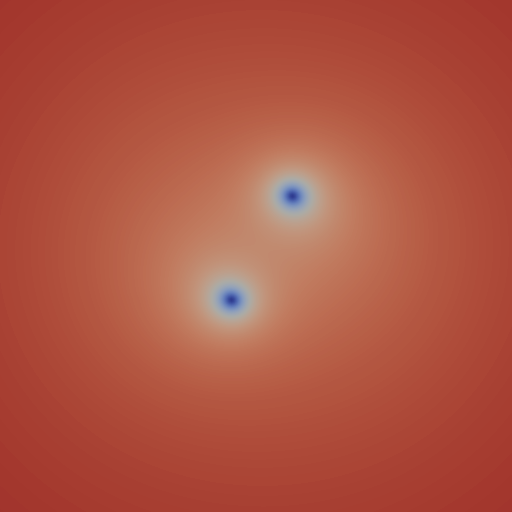
\includegraphics[width=2cm]{figs/gr_im1_r1.png}};
%		\end{scope}
%		%\begin{scope}[xshift=13.5cm,yshift=0.25cm]
%		%\node[anchor=south west,inner sep=0] at (0,0) {\includegraphics[width=2cm]{figs/gr_im_r1.png}};
%		%\end{scope}
%		
%		\begin{scope}[xshift=8cm,yshift=0.0cm,scale=0.025]
%		\draw [gray, ultra thin] (0.000000, 64.000000) rectangle +(8.000000,-8.000000);
\draw [gray, ultra thin] (8.000000, 64.000000) rectangle +(8.000000,-8.000000);
\draw [gray, ultra thin] (16.000000, 64.000000) rectangle +(8.000000,-8.000000);
\draw [gray, ultra thin] (24.000000, 64.000000) rectangle +(8.000000,-8.000000);
\draw [gray, ultra thin] (32.000000, 64.000000) rectangle +(8.000000,-8.000000);
\draw [gray, ultra thin] (40.000000, 64.000000) rectangle +(8.000000,-8.000000);
\draw [gray, ultra thin] (48.000000, 64.000000) rectangle +(8.000000,-8.000000);
\draw [gray, ultra thin] (56.000000, 64.000000) rectangle +(8.000000,-8.000000);
\draw [gray, ultra thin] (0.000000, 56.000000) rectangle +(8.000000,-8.000000);
\draw [gray, ultra thin] (8.000000, 56.000000) rectangle +(4.000000,-4.000000);
\draw [gray, ultra thin] (12.000000, 56.000000) rectangle +(4.000000,-4.000000);
\draw [gray, ultra thin] (16.000000, 56.000000) rectangle +(4.000000,-4.000000);
\draw [gray, ultra thin] (20.000000, 56.000000) rectangle +(4.000000,-4.000000);
\draw [gray, ultra thin] (24.000000, 56.000000) rectangle +(4.000000,-4.000000);
\draw [gray, ultra thin] (28.000000, 56.000000) rectangle +(4.000000,-4.000000);
\draw [gray, ultra thin] (32.000000, 56.000000) rectangle +(4.000000,-4.000000);
\draw [gray, ultra thin] (36.000000, 56.000000) rectangle +(4.000000,-4.000000);
\draw [gray, ultra thin] (40.000000, 56.000000) rectangle +(4.000000,-4.000000);
\draw [gray, ultra thin] (44.000000, 56.000000) rectangle +(4.000000,-4.000000);
\draw [gray, ultra thin] (48.000000, 56.000000) rectangle +(4.000000,-4.000000);
\draw [gray, ultra thin] (52.000000, 56.000000) rectangle +(4.000000,-4.000000);
\draw [gray, ultra thin] (56.000000, 56.000000) rectangle +(8.000000,-8.000000);
\draw [gray, ultra thin] (8.000000, 52.000000) rectangle +(4.000000,-4.000000);
\draw [gray, ultra thin] (12.000000, 52.000000) rectangle +(4.000000,-4.000000);
\draw [gray, ultra thin] (16.000000, 52.000000) rectangle +(4.000000,-4.000000);
\draw [gray, ultra thin] (20.000000, 52.000000) rectangle +(4.000000,-4.000000);
\draw [gray, ultra thin] (24.000000, 52.000000) rectangle +(4.000000,-4.000000);
\draw [gray, ultra thin] (28.000000, 52.000000) rectangle +(4.000000,-4.000000);
\draw [gray, ultra thin] (32.000000, 52.000000) rectangle +(4.000000,-4.000000);
\draw [gray, ultra thin] (36.000000, 52.000000) rectangle +(4.000000,-4.000000);
\draw [gray, ultra thin] (40.000000, 52.000000) rectangle +(4.000000,-4.000000);
\draw [gray, ultra thin] (44.000000, 52.000000) rectangle +(4.000000,-4.000000);
\draw [gray, ultra thin] (48.000000, 52.000000) rectangle +(4.000000,-4.000000);
\draw [gray, ultra thin] (52.000000, 52.000000) rectangle +(4.000000,-4.000000);
\draw [gray, ultra thin] (0.000000, 48.000000) rectangle +(4.000000,-4.000000);
\draw [gray, ultra thin] (4.000000, 48.000000) rectangle +(4.000000,-4.000000);
\draw [gray, ultra thin] (8.000000, 48.000000) rectangle +(4.000000,-4.000000);
\draw [gray, ultra thin] (12.000000, 48.000000) rectangle +(4.000000,-4.000000);
\draw [gray, ultra thin] (16.000000, 48.000000) rectangle +(4.000000,-4.000000);
\draw [gray, ultra thin] (20.000000, 48.000000) rectangle +(2.000000,-2.000000);
\draw [gray, ultra thin] (22.000000, 48.000000) rectangle +(2.000000,-2.000000);
\draw [gray, ultra thin] (24.000000, 48.000000) rectangle +(4.000000,-4.000000);
\draw [gray, ultra thin] (28.000000, 48.000000) rectangle +(4.000000,-4.000000);
\draw [gray, ultra thin] (32.000000, 48.000000) rectangle +(4.000000,-4.000000);
\draw [gray, ultra thin] (36.000000, 48.000000) rectangle +(4.000000,-4.000000);
\draw [gray, ultra thin] (40.000000, 48.000000) rectangle +(2.000000,-2.000000);
\draw [gray, ultra thin] (42.000000, 48.000000) rectangle +(2.000000,-2.000000);
\draw [gray, ultra thin] (44.000000, 48.000000) rectangle +(4.000000,-4.000000);
\draw [gray, ultra thin] (48.000000, 48.000000) rectangle +(4.000000,-4.000000);
\draw [gray, ultra thin] (52.000000, 48.000000) rectangle +(4.000000,-4.000000);
\draw [gray, ultra thin] (56.000000, 48.000000) rectangle +(4.000000,-4.000000);
\draw [gray, ultra thin] (60.000000, 48.000000) rectangle +(4.000000,-4.000000);
\draw [gray, ultra thin] (20.000000, 46.000000) rectangle +(2.000000,-2.000000);
\draw [gray, ultra thin] (22.000000, 46.000000) rectangle +(2.000000,-2.000000);
\draw [gray, ultra thin] (40.000000, 46.000000) rectangle +(2.000000,-2.000000);
\draw [gray, ultra thin] (42.000000, 46.000000) rectangle +(2.000000,-2.000000);
\draw [gray, ultra thin] (0.000000, 44.000000) rectangle +(4.000000,-4.000000);
\draw [gray, ultra thin] (4.000000, 44.000000) rectangle +(4.000000,-4.000000);
\draw [gray, ultra thin] (8.000000, 44.000000) rectangle +(4.000000,-4.000000);
\draw [gray, ultra thin] (12.000000, 44.000000) rectangle +(2.000000,-2.000000);
\draw [gray, ultra thin] (14.000000, 44.000000) rectangle +(2.000000,-2.000000);
\draw [gray, ultra thin] (16.000000, 44.000000) rectangle +(2.000000,-2.000000);
\draw [gray, ultra thin] (18.000000, 44.000000) rectangle +(2.000000,-2.000000);
\draw [gray, ultra thin] (20.000000, 44.000000) rectangle +(2.000000,-2.000000);
\draw [gray, ultra thin] (22.000000, 44.000000) rectangle +(2.000000,-2.000000);
\draw [gray, ultra thin] (24.000000, 44.000000) rectangle +(2.000000,-2.000000);
\draw [gray, ultra thin] (26.000000, 44.000000) rectangle +(2.000000,-2.000000);
\draw [gray, ultra thin] (28.000000, 44.000000) rectangle +(4.000000,-4.000000);
\draw [gray, ultra thin] (32.000000, 44.000000) rectangle +(4.000000,-4.000000);
\draw [gray, ultra thin] (36.000000, 44.000000) rectangle +(2.000000,-2.000000);
\draw [gray, ultra thin] (38.000000, 44.000000) rectangle +(2.000000,-2.000000);
\draw [gray, ultra thin] (40.000000, 44.000000) rectangle +(2.000000,-2.000000);
\draw [gray, ultra thin] (42.000000, 44.000000) rectangle +(2.000000,-2.000000);
\draw [gray, ultra thin] (44.000000, 44.000000) rectangle +(2.000000,-2.000000);
\draw [gray, ultra thin] (46.000000, 44.000000) rectangle +(2.000000,-2.000000);
\draw [gray, ultra thin] (48.000000, 44.000000) rectangle +(2.000000,-2.000000);
\draw [gray, ultra thin] (50.000000, 44.000000) rectangle +(2.000000,-2.000000);
\draw [gray, ultra thin] (52.000000, 44.000000) rectangle +(4.000000,-4.000000);
\draw [gray, ultra thin] (56.000000, 44.000000) rectangle +(4.000000,-4.000000);
\draw [gray, ultra thin] (60.000000, 44.000000) rectangle +(4.000000,-4.000000);
\draw [gray, ultra thin] (12.000000, 42.000000) rectangle +(2.000000,-2.000000);
\draw [gray, ultra thin] (14.000000, 42.000000) rectangle +(2.000000,-2.000000);
\draw [gray, ultra thin] (16.000000, 42.000000) rectangle +(2.000000,-2.000000);
\draw [gray, ultra thin] (18.000000, 42.000000) rectangle +(2.000000,-2.000000);
\draw [gray, ultra thin] (20.000000, 42.000000) rectangle +(2.000000,-2.000000);
\draw [gray, ultra thin] (22.000000, 42.000000) rectangle +(2.000000,-2.000000);
\draw [gray, ultra thin] (24.000000, 42.000000) rectangle +(2.000000,-2.000000);
\draw [gray, ultra thin] (26.000000, 42.000000) rectangle +(2.000000,-2.000000);
\draw [gray, ultra thin] (36.000000, 42.000000) rectangle +(2.000000,-2.000000);
\draw [gray, ultra thin] (38.000000, 42.000000) rectangle +(2.000000,-2.000000);
\draw [gray, ultra thin] (40.000000, 42.000000) rectangle +(2.000000,-2.000000);
\draw [gray, ultra thin] (42.000000, 42.000000) rectangle +(2.000000,-2.000000);
\draw [gray, ultra thin] (44.000000, 42.000000) rectangle +(2.000000,-2.000000);
\draw [gray, ultra thin] (46.000000, 42.000000) rectangle +(2.000000,-2.000000);
\draw [gray, ultra thin] (48.000000, 42.000000) rectangle +(2.000000,-2.000000);
\draw [gray, ultra thin] (50.000000, 42.000000) rectangle +(2.000000,-2.000000);
\draw [gray, ultra thin] (0.000000, 40.000000) rectangle +(8.000000,-8.000000);
\draw [gray, ultra thin] (8.000000, 40.000000) rectangle +(4.000000,-4.000000);
\draw [gray, ultra thin] (12.000000, 40.000000) rectangle +(2.000000,-2.000000);
\draw [gray, ultra thin] (14.000000, 40.000000) rectangle +(2.000000,-2.000000);
\draw [gray, ultra thin] (16.000000, 40.000000) rectangle +(2.000000,-2.000000);
\draw [gray, ultra thin] (18.000000, 40.000000) rectangle +(2.000000,-2.000000);
\draw [gray, ultra thin] (20.000000, 40.000000) rectangle +(2.000000,-2.000000);
\draw [gray, ultra thin] (22.000000, 40.000000) rectangle +(2.000000,-2.000000);
\draw [gray, ultra thin] (24.000000, 40.000000) rectangle +(2.000000,-2.000000);
\draw [gray, ultra thin] (26.000000, 40.000000) rectangle +(2.000000,-2.000000);
\draw [gray, ultra thin] (28.000000, 40.000000) rectangle +(2.000000,-2.000000);
\draw [gray, ultra thin] (30.000000, 40.000000) rectangle +(2.000000,-2.000000);
\draw [gray, ultra thin] (32.000000, 40.000000) rectangle +(2.000000,-2.000000);
\draw [gray, ultra thin] (34.000000, 40.000000) rectangle +(2.000000,-2.000000);
\draw [gray, ultra thin] (36.000000, 40.000000) rectangle +(2.000000,-2.000000);
\draw [gray, ultra thin] (38.000000, 40.000000) rectangle +(2.000000,-2.000000);
\draw [gray, ultra thin] (40.000000, 40.000000) rectangle +(2.000000,-2.000000);
\draw [gray, ultra thin] (42.000000, 40.000000) rectangle +(2.000000,-2.000000);
\draw [gray, ultra thin] (44.000000, 40.000000) rectangle +(2.000000,-2.000000);
\draw [gray, ultra thin] (46.000000, 40.000000) rectangle +(2.000000,-2.000000);
\draw [gray, ultra thin] (48.000000, 40.000000) rectangle +(2.000000,-2.000000);
\draw [gray, ultra thin] (50.000000, 40.000000) rectangle +(2.000000,-2.000000);
\draw [gray, ultra thin] (52.000000, 40.000000) rectangle +(4.000000,-4.000000);
\draw [gray, ultra thin] (56.000000, 40.000000) rectangle +(4.000000,-4.000000);
\draw [gray, ultra thin] (60.000000, 40.000000) rectangle +(4.000000,-4.000000);
\draw [gray, ultra thin] (12.000000, 38.000000) rectangle +(2.000000,-2.000000);
\draw [gray, ultra thin] (14.000000, 38.000000) rectangle +(2.000000,-2.000000);
\draw [gray, ultra thin] (16.000000, 38.000000) rectangle +(2.000000,-2.000000);
\draw [gray, ultra thin] (18.000000, 38.000000) rectangle +(1.000000,-1.000000);
\draw [gray, ultra thin] (19.000000, 38.000000) rectangle +(1.000000,-1.000000);
\draw [gray, ultra thin] (20.000000, 38.000000) rectangle +(1.000000,-1.000000);
\draw [gray, ultra thin] (21.000000, 38.000000) rectangle +(1.000000,-1.000000);
\draw [gray, ultra thin] (22.000000, 38.000000) rectangle +(1.000000,-1.000000);
\draw [gray, ultra thin] (23.000000, 38.000000) rectangle +(1.000000,-1.000000);
\draw [gray, ultra thin] (24.000000, 38.000000) rectangle +(2.000000,-2.000000);
\draw [gray, ultra thin] (26.000000, 38.000000) rectangle +(2.000000,-2.000000);
\draw [gray, ultra thin] (28.000000, 38.000000) rectangle +(2.000000,-2.000000);
\draw [gray, ultra thin] (30.000000, 38.000000) rectangle +(2.000000,-2.000000);
\draw [gray, ultra thin] (32.000000, 38.000000) rectangle +(2.000000,-2.000000);
\draw [gray, ultra thin] (34.000000, 38.000000) rectangle +(2.000000,-2.000000);
\draw [gray, ultra thin] (36.000000, 38.000000) rectangle +(2.000000,-2.000000);
\draw [gray, ultra thin] (38.000000, 38.000000) rectangle +(2.000000,-2.000000);
\draw [gray, ultra thin] (40.000000, 38.000000) rectangle +(1.000000,-1.000000);
\draw [gray, ultra thin] (41.000000, 38.000000) rectangle +(1.000000,-1.000000);
\draw [gray, ultra thin] (42.000000, 38.000000) rectangle +(1.000000,-1.000000);
\draw [gray, ultra thin] (43.000000, 38.000000) rectangle +(1.000000,-1.000000);
\draw [gray, ultra thin] (44.000000, 38.000000) rectangle +(2.000000,-2.000000);
\draw [gray, ultra thin] (46.000000, 38.000000) rectangle +(2.000000,-2.000000);
\draw [gray, ultra thin] (48.000000, 38.000000) rectangle +(2.000000,-2.000000);
\draw [gray, ultra thin] (50.000000, 38.000000) rectangle +(2.000000,-2.000000);
\draw [gray, ultra thin] (18.000000, 37.000000) rectangle +(1.000000,-1.000000);
\draw [gray, ultra thin] (19.000000, 37.000000) rectangle +(1.000000,-1.000000);
\draw [gray, ultra thin] (20.000000, 37.000000) rectangle +(1.000000,-1.000000);
\draw [gray, ultra thin] (21.000000, 37.000000) rectangle +(1.000000,-1.000000);
\draw [gray, ultra thin] (22.000000, 37.000000) rectangle +(1.000000,-1.000000);
\draw [gray, ultra thin] (23.000000, 37.000000) rectangle +(1.000000,-1.000000);
\draw [gray, ultra thin] (40.000000, 37.000000) rectangle +(1.000000,-1.000000);
\draw [gray, ultra thin] (41.000000, 37.000000) rectangle +(1.000000,-1.000000);
\draw [gray, ultra thin] (42.000000, 37.000000) rectangle +(1.000000,-1.000000);
\draw [gray, ultra thin] (43.000000, 37.000000) rectangle +(1.000000,-1.000000);
\draw [gray, ultra thin] (8.000000, 36.000000) rectangle +(4.000000,-4.000000);
\draw [gray, ultra thin] (12.000000, 36.000000) rectangle +(2.000000,-2.000000);
\draw [gray, ultra thin] (14.000000, 36.000000) rectangle +(2.000000,-2.000000);
\draw [gray, ultra thin] (16.000000, 36.000000) rectangle +(1.000000,-1.000000);
\draw [gray, ultra thin] (17.000000, 36.000000) rectangle +(1.000000,-1.000000);
\draw [gray, ultra thin] (18.000000, 36.000000) rectangle +(1.000000,-1.000000);
\draw [gray, ultra thin] (19.000000, 36.000000) rectangle +(1.000000,-1.000000);
\draw [gray, ultra thin] (20.000000, 36.000000) rectangle +(1.000000,-1.000000);
\draw [gray, ultra thin] (21.000000, 36.000000) rectangle +(1.000000,-1.000000);
\draw [gray, ultra thin] (22.000000, 36.000000) rectangle +(2.000000,-2.000000);
\draw [gray, ultra thin] (24.000000, 36.000000) rectangle +(2.000000,-2.000000);
\draw [gray, ultra thin] (26.000000, 36.000000) rectangle +(2.000000,-2.000000);
\draw [gray, ultra thin] (28.000000, 36.000000) rectangle +(2.000000,-2.000000);
\draw [gray, ultra thin] (30.000000, 36.000000) rectangle +(2.000000,-2.000000);
\draw [gray, ultra thin] (32.000000, 36.000000) rectangle +(2.000000,-2.000000);
\draw [gray, ultra thin] (34.000000, 36.000000) rectangle +(2.000000,-2.000000);
\draw [gray, ultra thin] (36.000000, 36.000000) rectangle +(2.000000,-2.000000);
\draw [gray, ultra thin] (38.000000, 36.000000) rectangle +(2.000000,-2.000000);
\draw [gray, ultra thin] (40.000000, 36.000000) rectangle +(2.000000,-2.000000);
\draw [gray, ultra thin] (42.000000, 36.000000) rectangle +(1.000000,-1.000000);
\draw [gray, ultra thin] (43.000000, 36.000000) rectangle +(1.000000,-1.000000);
\draw [gray, ultra thin] (44.000000, 36.000000) rectangle +(1.000000,-1.000000);
\draw [gray, ultra thin] (45.000000, 36.000000) rectangle +(1.000000,-1.000000);
\draw [gray, ultra thin] (46.000000, 36.000000) rectangle +(2.000000,-2.000000);
\draw [gray, ultra thin] (48.000000, 36.000000) rectangle +(2.000000,-2.000000);
\draw [gray, ultra thin] (50.000000, 36.000000) rectangle +(2.000000,-2.000000);
\draw [gray, ultra thin] (52.000000, 36.000000) rectangle +(4.000000,-4.000000);
\draw [gray, ultra thin] (56.000000, 36.000000) rectangle +(4.000000,-4.000000);
\draw [gray, ultra thin] (60.000000, 36.000000) rectangle +(4.000000,-4.000000);
\draw [gray, ultra thin] (16.000000, 35.000000) rectangle +(1.000000,-1.000000);
\draw [gray, ultra thin] (17.000000, 35.000000) rectangle +(1.000000,-1.000000);
\draw [gray, ultra thin] (18.000000, 35.000000) rectangle +(1.000000,-1.000000);
\draw [gray, ultra thin] (19.000000, 35.000000) rectangle +(1.000000,-1.000000);
\draw [gray, ultra thin] (20.000000, 35.000000) rectangle +(1.000000,-1.000000);
\draw [gray, ultra thin] (21.000000, 35.000000) rectangle +(1.000000,-1.000000);
\draw [gray, ultra thin] (42.000000, 35.000000) rectangle +(1.000000,-1.000000);
\draw [gray, ultra thin] (43.000000, 35.000000) rectangle +(1.000000,-1.000000);
\draw [gray, ultra thin] (44.000000, 35.000000) rectangle +(1.000000,-1.000000);
\draw [gray, ultra thin] (45.000000, 35.000000) rectangle +(1.000000,-1.000000);
\draw [gray, ultra thin] (12.000000, 34.000000) rectangle +(2.000000,-2.000000);
\draw [gray, ultra thin] (14.000000, 34.000000) rectangle +(2.000000,-2.000000);
\draw [gray, ultra thin] (16.000000, 34.000000) rectangle +(2.000000,-2.000000);
\draw [gray, ultra thin] (18.000000, 34.000000) rectangle +(1.000000,-1.000000);
\draw [gray, ultra thin] (19.000000, 34.000000) rectangle +(1.000000,-1.000000);
\draw [gray, ultra thin] (20.000000, 34.000000) rectangle +(2.000000,-2.000000);
\draw [gray, ultra thin] (22.000000, 34.000000) rectangle +(0.500000,-0.500000);
\draw [gray, ultra thin] (22.500000, 34.000000) rectangle +(0.500000,-0.500000);
\draw [gray, ultra thin] (23.000000, 34.000000) rectangle +(0.500000,-0.500000);
\draw [gray, ultra thin] (23.500000, 34.000000) rectangle +(0.500000,-0.500000);
\draw [gray, ultra thin] (24.000000, 34.000000) rectangle +(0.500000,-0.500000);
\draw [gray, ultra thin] (24.500000, 34.000000) rectangle +(0.500000,-0.500000);
\draw [gray, ultra thin] (25.000000, 34.000000) rectangle +(0.500000,-0.500000);
\draw [gray, ultra thin] (25.500000, 34.000000) rectangle +(0.500000,-0.500000);
\draw [gray, ultra thin] (26.000000, 34.000000) rectangle +(2.000000,-2.000000);
\draw [gray, ultra thin] (28.000000, 34.000000) rectangle +(2.000000,-2.000000);
\draw [gray, ultra thin] (30.000000, 34.000000) rectangle +(2.000000,-2.000000);
\draw [gray, ultra thin] (32.000000, 34.000000) rectangle +(2.000000,-2.000000);
\draw [gray, ultra thin] (34.000000, 34.000000) rectangle +(2.000000,-2.000000);
\draw [gray, ultra thin] (36.000000, 34.000000) rectangle +(1.000000,-1.000000);
\draw [gray, ultra thin] (37.000000, 34.000000) rectangle +(1.000000,-1.000000);
\draw [gray, ultra thin] (38.000000, 34.000000) rectangle +(0.500000,-0.500000);
\draw [gray, ultra thin] (38.500000, 34.000000) rectangle +(0.500000,-0.500000);
\draw [gray, ultra thin] (39.000000, 34.000000) rectangle +(0.500000,-0.500000);
\draw [gray, ultra thin] (39.500000, 34.000000) rectangle +(0.500000,-0.500000);
\draw [gray, ultra thin] (40.000000, 34.000000) rectangle +(0.500000,-0.500000);
\draw [gray, ultra thin] (40.500000, 34.000000) rectangle +(0.500000,-0.500000);
\draw [gray, ultra thin] (41.000000, 34.000000) rectangle +(1.000000,-1.000000);
\draw [gray, ultra thin] (42.000000, 34.000000) rectangle +(2.000000,-2.000000);
\draw [gray, ultra thin] (44.000000, 34.000000) rectangle +(1.000000,-1.000000);
\draw [gray, ultra thin] (45.000000, 34.000000) rectangle +(1.000000,-1.000000);
\draw [gray, ultra thin] (46.000000, 34.000000) rectangle +(2.000000,-2.000000);
\draw [gray, ultra thin] (48.000000, 34.000000) rectangle +(2.000000,-2.000000);
\draw [gray, ultra thin] (50.000000, 34.000000) rectangle +(2.000000,-2.000000);
\draw [gray, ultra thin] (22.000000, 33.500000) rectangle +(0.500000,-0.500000);
\draw [gray, ultra thin] (22.500000, 33.500000) rectangle +(0.500000,-0.500000);
\draw [gray, ultra thin] (23.000000, 33.500000) rectangle +(0.250000,-0.250000);
\draw [gray, ultra thin] (23.250000, 33.500000) rectangle +(0.250000,-0.250000);
\draw [gray, ultra thin] (23.500000, 33.500000) rectangle +(0.250000,-0.250000);
\draw [gray, ultra thin] (23.750000, 33.500000) rectangle +(0.250000,-0.250000);
\draw [gray, ultra thin] (24.000000, 33.500000) rectangle +(0.500000,-0.500000);
\draw [gray, ultra thin] (24.500000, 33.500000) rectangle +(0.250000,-0.250000);
\draw [gray, ultra thin] (24.750000, 33.500000) rectangle +(0.250000,-0.250000);
\draw [gray, ultra thin] (25.000000, 33.500000) rectangle +(0.500000,-0.500000);
\draw [gray, ultra thin] (25.500000, 33.500000) rectangle +(0.500000,-0.500000);
\draw [gray, ultra thin] (38.000000, 33.500000) rectangle +(0.500000,-0.500000);
\draw [gray, ultra thin] (38.500000, 33.500000) rectangle +(0.500000,-0.500000);
\draw [gray, ultra thin] (39.000000, 33.500000) rectangle +(0.500000,-0.500000);
\draw [gray, ultra thin] (39.500000, 33.500000) rectangle +(0.250000,-0.250000);
\draw [gray, ultra thin] (39.750000, 33.500000) rectangle +(0.250000,-0.250000);
\draw [gray, ultra thin] (40.000000, 33.500000) rectangle +(0.250000,-0.250000);
\draw [gray, ultra thin] (40.250000, 33.500000) rectangle +(0.250000,-0.250000);
\draw [gray, ultra thin] (40.500000, 33.500000) rectangle +(0.500000,-0.500000);
\draw [gray, ultra thin] (23.000000, 33.250000) rectangle +(0.250000,-0.250000);
\draw [gray, ultra thin] (23.250000, 33.250000) rectangle +(0.250000,-0.250000);
\draw [gray, ultra thin] (23.500000, 33.250000) rectangle +(0.250000,-0.250000);
\draw [gray, ultra thin] (23.750000, 33.250000) rectangle +(0.250000,-0.250000);
\draw [gray, ultra thin] (24.500000, 33.250000) rectangle +(0.250000,-0.250000);
\draw [gray, ultra thin] (24.750000, 33.250000) rectangle +(0.250000,-0.250000);
\draw [gray, ultra thin] (39.500000, 33.250000) rectangle +(0.250000,-0.250000);
\draw [gray, ultra thin] (39.750000, 33.250000) rectangle +(0.250000,-0.250000);
\draw [gray, ultra thin] (40.000000, 33.250000) rectangle +(0.250000,-0.250000);
\draw [gray, ultra thin] (40.250000, 33.250000) rectangle +(0.250000,-0.250000);
\draw [gray, ultra thin] (18.000000, 33.000000) rectangle +(1.000000,-1.000000);
\draw [gray, ultra thin] (19.000000, 33.000000) rectangle +(1.000000,-1.000000);
\draw [gray, ultra thin] (22.000000, 33.000000) rectangle +(0.500000,-0.500000);
\draw [gray, ultra thin] (22.500000, 33.000000) rectangle +(0.250000,-0.250000);
\draw [gray, ultra thin] (22.750000, 33.000000) rectangle +(0.250000,-0.250000);
\draw [gray, ultra thin] (23.000000, 33.000000) rectangle +(0.250000,-0.250000);
\draw [gray, ultra thin] (23.250000, 33.000000) rectangle +(0.250000,-0.250000);
\draw [gray, ultra thin] (23.500000, 33.000000) rectangle +(0.250000,-0.250000);
\draw [gray, ultra thin] (23.750000, 33.000000) rectangle +(0.250000,-0.250000);
\draw [gray, ultra thin] (24.000000, 33.000000) rectangle +(0.250000,-0.250000);
\draw [gray, ultra thin] (24.250000, 33.000000) rectangle +(0.250000,-0.250000);
\draw [gray, ultra thin] (24.500000, 33.000000) rectangle +(0.250000,-0.250000);
\draw [gray, ultra thin] (24.750000, 33.000000) rectangle +(0.250000,-0.250000);
\draw [gray, ultra thin] (25.000000, 33.000000) rectangle +(0.250000,-0.250000);
\draw [gray, ultra thin] (25.250000, 33.000000) rectangle +(0.250000,-0.250000);
\draw [gray, ultra thin] (25.500000, 33.000000) rectangle +(0.500000,-0.500000);
\draw [gray, ultra thin] (36.000000, 33.000000) rectangle +(1.000000,-1.000000);
\draw [gray, ultra thin] (37.000000, 33.000000) rectangle +(0.500000,-0.500000);
\draw [gray, ultra thin] (37.500000, 33.000000) rectangle +(0.500000,-0.500000);
\draw [gray, ultra thin] (38.000000, 33.000000) rectangle +(0.250000,-0.250000);
\draw [gray, ultra thin] (38.250000, 33.000000) rectangle +(0.250000,-0.250000);
\draw [gray, ultra thin] (38.500000, 33.000000) rectangle +(0.250000,-0.250000);
\draw [gray, ultra thin] (38.750000, 33.000000) rectangle +(0.250000,-0.250000);
\draw [gray, ultra thin] (39.000000, 33.000000) rectangle +(0.250000,-0.250000);
\draw [gray, ultra thin] (39.250000, 33.000000) rectangle +(0.250000,-0.250000);
\draw [gray, ultra thin] (39.500000, 33.000000) rectangle +(0.250000,-0.250000);
\draw [gray, ultra thin] (39.750000, 33.000000) rectangle +(0.250000,-0.250000);
\draw [gray, ultra thin] (40.000000, 33.000000) rectangle +(0.250000,-0.250000);
\draw [gray, ultra thin] (40.250000, 33.000000) rectangle +(0.250000,-0.250000);
\draw [gray, ultra thin] (40.500000, 33.000000) rectangle +(0.250000,-0.250000);
\draw [gray, ultra thin] (40.750000, 33.000000) rectangle +(0.250000,-0.250000);
\draw [gray, ultra thin] (41.000000, 33.000000) rectangle +(0.500000,-0.500000);
\draw [gray, ultra thin] (41.500000, 33.000000) rectangle +(0.500000,-0.500000);
\draw [gray, ultra thin] (44.000000, 33.000000) rectangle +(1.000000,-1.000000);
\draw [gray, ultra thin] (45.000000, 33.000000) rectangle +(1.000000,-1.000000);
\draw [gray, ultra thin] (22.500000, 32.750000) rectangle +(0.250000,-0.250000);
\draw [gray, ultra thin] (22.750000, 32.750000) rectangle +(0.250000,-0.250000);
\draw [gray, ultra thin] (23.000000, 32.750000) rectangle +(0.250000,-0.250000);
\draw [gray, ultra thin] (23.250000, 32.750000) rectangle +(0.250000,-0.250000);
\draw [gray, ultra thin] (23.500000, 32.750000) rectangle +(0.250000,-0.250000);
\draw [gray, ultra thin] (23.750000, 32.750000) rectangle +(0.250000,-0.250000);
\draw [gray, ultra thin] (24.000000, 32.750000) rectangle +(0.250000,-0.250000);
\draw [gray, ultra thin] (24.250000, 32.750000) rectangle +(0.250000,-0.250000);
\draw [gray, ultra thin] (24.500000, 32.750000) rectangle +(0.250000,-0.250000);
\draw [gray, ultra thin] (24.750000, 32.750000) rectangle +(0.250000,-0.250000);
\draw [gray, ultra thin] (25.000000, 32.750000) rectangle +(0.250000,-0.250000);
\draw [gray, ultra thin] (25.250000, 32.750000) rectangle +(0.250000,-0.250000);
\draw [gray, ultra thin] (38.000000, 32.750000) rectangle +(0.250000,-0.250000);
\draw [gray, ultra thin] (38.250000, 32.750000) rectangle +(0.250000,-0.250000);
\draw [gray, ultra thin] (38.500000, 32.750000) rectangle +(0.250000,-0.250000);
\draw [gray, ultra thin] (38.750000, 32.750000) rectangle +(0.250000,-0.250000);
\draw [gray, ultra thin] (39.000000, 32.750000) rectangle +(0.250000,-0.250000);
\draw [gray, ultra thin] (39.250000, 32.750000) rectangle +(0.250000,-0.250000);
\draw [gray, ultra thin] (39.500000, 32.750000) rectangle +(0.250000,-0.250000);
\draw [gray, ultra thin] (39.750000, 32.750000) rectangle +(0.250000,-0.250000);
\draw [gray, ultra thin] (40.000000, 32.750000) rectangle +(0.250000,-0.250000);
\draw [gray, ultra thin] (40.250000, 32.750000) rectangle +(0.250000,-0.250000);
\draw [gray, ultra thin] (40.500000, 32.750000) rectangle +(0.250000,-0.250000);
\draw [gray, ultra thin] (40.750000, 32.750000) rectangle +(0.250000,-0.250000);
\draw [gray, ultra thin] (22.000000, 32.500000) rectangle +(0.500000,-0.500000);
\draw [gray, ultra thin] (22.500000, 32.500000) rectangle +(0.250000,-0.250000);
\draw [gray, ultra thin] (22.750000, 32.500000) rectangle +(0.250000,-0.250000);
\draw [gray, ultra thin] (23.000000, 32.500000) rectangle +(0.250000,-0.250000);
\draw [gray, ultra thin] (23.250000, 32.500000) rectangle +(0.250000,-0.250000);
\draw [gray, ultra thin] (23.500000, 32.500000) rectangle +(0.250000,-0.250000);
\draw [gray, ultra thin] (23.750000, 32.500000) rectangle +(0.250000,-0.250000);
\draw [gray, ultra thin] (24.000000, 32.500000) rectangle +(0.250000,-0.250000);
\draw [gray, ultra thin] (24.250000, 32.500000) rectangle +(0.250000,-0.250000);
\draw [gray, ultra thin] (24.500000, 32.500000) rectangle +(0.250000,-0.250000);
\draw [gray, ultra thin] (24.750000, 32.500000) rectangle +(0.250000,-0.250000);
\draw [gray, ultra thin] (25.000000, 32.500000) rectangle +(0.250000,-0.250000);
\draw [gray, ultra thin] (25.250000, 32.500000) rectangle +(0.250000,-0.250000);
\draw [gray, ultra thin] (25.500000, 32.500000) rectangle +(0.500000,-0.500000);
\draw [gray, ultra thin] (37.000000, 32.500000) rectangle +(0.500000,-0.500000);
\draw [gray, ultra thin] (37.500000, 32.500000) rectangle +(0.500000,-0.500000);
\draw [gray, ultra thin] (38.000000, 32.500000) rectangle +(0.250000,-0.250000);
\draw [gray, ultra thin] (38.250000, 32.500000) rectangle +(0.250000,-0.250000);
\draw [gray, ultra thin] (38.500000, 32.500000) rectangle +(0.250000,-0.250000);
\draw [gray, ultra thin] (38.750000, 32.500000) rectangle +(0.250000,-0.250000);
\draw [gray, ultra thin] (39.000000, 32.500000) rectangle +(0.250000,-0.250000);
\draw [gray, ultra thin] (39.250000, 32.500000) rectangle +(0.250000,-0.250000);
\draw [gray, ultra thin] (39.500000, 32.500000) rectangle +(0.250000,-0.250000);
\draw [gray, ultra thin] (39.750000, 32.500000) rectangle +(0.250000,-0.250000);
\draw [gray, ultra thin] (40.000000, 32.500000) rectangle +(0.250000,-0.250000);
\draw [gray, ultra thin] (40.250000, 32.500000) rectangle +(0.250000,-0.250000);
\draw [gray, ultra thin] (40.500000, 32.500000) rectangle +(0.250000,-0.250000);
\draw [gray, ultra thin] (40.750000, 32.500000) rectangle +(0.250000,-0.250000);
\draw [gray, ultra thin] (41.000000, 32.500000) rectangle +(0.500000,-0.500000);
\draw [gray, ultra thin] (41.500000, 32.500000) rectangle +(0.500000,-0.500000);
\draw [gray, ultra thin] (22.500000, 32.250000) rectangle +(0.250000,-0.250000);
\draw [gray, ultra thin] (22.750000, 32.250000) rectangle +(0.250000,-0.250000);
\draw [gray, ultra thin] (23.000000, 32.250000) rectangle +(0.250000,-0.250000);
\draw [gray, ultra thin] (23.250000, 32.250000) rectangle +(0.250000,-0.250000);
\draw [gray, ultra thin] (23.500000, 32.250000) rectangle +(0.125000,-0.125000);
\draw [gray, ultra thin] (23.625000, 32.250000) rectangle +(0.125000,-0.125000);
\draw [gray, ultra thin] (23.750000, 32.250000) rectangle +(0.250000,-0.250000);
\draw [gray, ultra thin] (24.000000, 32.250000) rectangle +(0.250000,-0.250000);
\draw [gray, ultra thin] (24.250000, 32.250000) rectangle +(0.125000,-0.125000);
\draw [gray, ultra thin] (24.375000, 32.250000) rectangle +(0.125000,-0.125000);
\draw [gray, ultra thin] (24.500000, 32.250000) rectangle +(0.250000,-0.250000);
\draw [gray, ultra thin] (24.750000, 32.250000) rectangle +(0.250000,-0.250000);
\draw [gray, ultra thin] (25.000000, 32.250000) rectangle +(0.250000,-0.250000);
\draw [gray, ultra thin] (25.250000, 32.250000) rectangle +(0.250000,-0.250000);
\draw [gray, ultra thin] (38.000000, 32.250000) rectangle +(0.250000,-0.250000);
\draw [gray, ultra thin] (38.250000, 32.250000) rectangle +(0.250000,-0.250000);
\draw [gray, ultra thin] (38.500000, 32.250000) rectangle +(0.250000,-0.250000);
\draw [gray, ultra thin] (38.750000, 32.250000) rectangle +(0.250000,-0.250000);
\draw [gray, ultra thin] (39.000000, 32.250000) rectangle +(0.125000,-0.125000);
\draw [gray, ultra thin] (39.125000, 32.250000) rectangle +(0.125000,-0.125000);
\draw [gray, ultra thin] (39.250000, 32.250000) rectangle +(0.250000,-0.250000);
\draw [gray, ultra thin] (39.500000, 32.250000) rectangle +(0.250000,-0.250000);
\draw [gray, ultra thin] (39.750000, 32.250000) rectangle +(0.125000,-0.125000);
\draw [gray, ultra thin] (39.875000, 32.250000) rectangle +(0.125000,-0.125000);
\draw [gray, ultra thin] (40.000000, 32.250000) rectangle +(0.250000,-0.250000);
\draw [gray, ultra thin] (40.250000, 32.250000) rectangle +(0.250000,-0.250000);
\draw [gray, ultra thin] (40.500000, 32.250000) rectangle +(0.250000,-0.250000);
\draw [gray, ultra thin] (40.750000, 32.250000) rectangle +(0.250000,-0.250000);
\draw [gray, ultra thin] (23.500000, 32.125000) rectangle +(0.125000,-0.125000);
\draw [gray, ultra thin] (23.625000, 32.125000) rectangle +(0.125000,-0.125000);
\draw [gray, ultra thin] (24.250000, 32.125000) rectangle +(0.125000,-0.125000);
\draw [gray, ultra thin] (24.375000, 32.125000) rectangle +(0.125000,-0.125000);
\draw [gray, ultra thin] (39.000000, 32.125000) rectangle +(0.125000,-0.125000);
\draw [gray, ultra thin] (39.125000, 32.125000) rectangle +(0.125000,-0.125000);
\draw [gray, ultra thin] (39.750000, 32.125000) rectangle +(0.125000,-0.125000);
\draw [gray, ultra thin] (39.875000, 32.125000) rectangle +(0.125000,-0.125000);
\draw [gray, ultra thin] (0.000000, 32.000000) rectangle +(8.000000,-8.000000);
\draw [gray, ultra thin] (8.000000, 32.000000) rectangle +(4.000000,-4.000000);
\draw [gray, ultra thin] (12.000000, 32.000000) rectangle +(2.000000,-2.000000);
\draw [gray, ultra thin] (14.000000, 32.000000) rectangle +(2.000000,-2.000000);
\draw [gray, ultra thin] (16.000000, 32.000000) rectangle +(2.000000,-2.000000);
\draw [gray, ultra thin] (18.000000, 32.000000) rectangle +(1.000000,-1.000000);
\draw [gray, ultra thin] (19.000000, 32.000000) rectangle +(1.000000,-1.000000);
\draw [gray, ultra thin] (20.000000, 32.000000) rectangle +(2.000000,-2.000000);
\draw [gray, ultra thin] (22.000000, 32.000000) rectangle +(0.500000,-0.500000);
\draw [gray, ultra thin] (22.500000, 32.000000) rectangle +(0.250000,-0.250000);
\draw [gray, ultra thin] (22.750000, 32.000000) rectangle +(0.250000,-0.250000);
\draw [gray, ultra thin] (23.000000, 32.000000) rectangle +(0.250000,-0.250000);
\draw [gray, ultra thin] (23.250000, 32.000000) rectangle +(0.125000,-0.125000);
\draw [gray, ultra thin] (23.375000, 32.000000) rectangle +(0.125000,-0.125000);
\draw [gray, ultra thin] (23.500000, 32.000000) rectangle +(0.250000,-0.250000);
\draw [gray, ultra thin] (23.750000, 32.000000) rectangle +(0.250000,-0.250000);
\draw [gray, ultra thin] (24.000000, 32.000000) rectangle +(0.250000,-0.250000);
\draw [gray, ultra thin] (24.250000, 32.000000) rectangle +(0.125000,-0.125000);
\draw [gray, ultra thin] (24.375000, 32.000000) rectangle +(0.125000,-0.125000);
\draw [gray, ultra thin] (24.500000, 32.000000) rectangle +(0.250000,-0.250000);
\draw [gray, ultra thin] (24.750000, 32.000000) rectangle +(0.250000,-0.250000);
\draw [gray, ultra thin] (25.000000, 32.000000) rectangle +(0.250000,-0.250000);
\draw [gray, ultra thin] (25.250000, 32.000000) rectangle +(0.250000,-0.250000);
\draw [gray, ultra thin] (25.500000, 32.000000) rectangle +(0.500000,-0.500000);
\draw [gray, ultra thin] (26.000000, 32.000000) rectangle +(2.000000,-2.000000);
\draw [gray, ultra thin] (28.000000, 32.000000) rectangle +(4.000000,-4.000000);
\draw [gray, ultra thin] (32.000000, 32.000000) rectangle +(4.000000,-4.000000);
\draw [gray, ultra thin] (36.000000, 32.000000) rectangle +(1.000000,-1.000000);
\draw [gray, ultra thin] (37.000000, 32.000000) rectangle +(0.500000,-0.500000);
\draw [gray, ultra thin] (37.500000, 32.000000) rectangle +(0.500000,-0.500000);
\draw [gray, ultra thin] (38.000000, 32.000000) rectangle +(0.250000,-0.250000);
\draw [gray, ultra thin] (38.250000, 32.000000) rectangle +(0.250000,-0.250000);
\draw [gray, ultra thin] (38.500000, 32.000000) rectangle +(0.250000,-0.250000);
\draw [gray, ultra thin] (38.750000, 32.000000) rectangle +(0.250000,-0.250000);
\draw [gray, ultra thin] (39.000000, 32.000000) rectangle +(0.125000,-0.125000);
\draw [gray, ultra thin] (39.125000, 32.000000) rectangle +(0.125000,-0.125000);
\draw [gray, ultra thin] (39.250000, 32.000000) rectangle +(0.250000,-0.250000);
\draw [gray, ultra thin] (39.500000, 32.000000) rectangle +(0.250000,-0.250000);
\draw [gray, ultra thin] (39.750000, 32.000000) rectangle +(0.250000,-0.250000);
\draw [gray, ultra thin] (40.000000, 32.000000) rectangle +(0.250000,-0.250000);
\draw [gray, ultra thin] (40.250000, 32.000000) rectangle +(0.250000,-0.250000);
\draw [gray, ultra thin] (40.500000, 32.000000) rectangle +(0.250000,-0.250000);
\draw [gray, ultra thin] (40.750000, 32.000000) rectangle +(0.250000,-0.250000);
\draw [gray, ultra thin] (41.000000, 32.000000) rectangle +(0.500000,-0.500000);
\draw [gray, ultra thin] (41.500000, 32.000000) rectangle +(0.500000,-0.500000);
\draw [gray, ultra thin] (42.000000, 32.000000) rectangle +(2.000000,-2.000000);
\draw [gray, ultra thin] (44.000000, 32.000000) rectangle +(1.000000,-1.000000);
\draw [gray, ultra thin] (45.000000, 32.000000) rectangle +(1.000000,-1.000000);
\draw [gray, ultra thin] (46.000000, 32.000000) rectangle +(2.000000,-2.000000);
\draw [gray, ultra thin] (48.000000, 32.000000) rectangle +(2.000000,-2.000000);
\draw [gray, ultra thin] (50.000000, 32.000000) rectangle +(2.000000,-2.000000);
\draw [gray, ultra thin] (52.000000, 32.000000) rectangle +(4.000000,-4.000000);
\draw [gray, ultra thin] (56.000000, 32.000000) rectangle +(4.000000,-4.000000);
\draw [gray, ultra thin] (60.000000, 32.000000) rectangle +(4.000000,-4.000000);
\draw [gray, ultra thin] (23.250000, 31.875000) rectangle +(0.125000,-0.125000);
\draw [gray, ultra thin] (23.375000, 31.875000) rectangle +(0.125000,-0.125000);
\draw [gray, ultra thin] (24.250000, 31.875000) rectangle +(0.125000,-0.125000);
\draw [gray, ultra thin] (24.375000, 31.875000) rectangle +(0.125000,-0.125000);
\draw [gray, ultra thin] (39.000000, 31.875000) rectangle +(0.125000,-0.125000);
\draw [gray, ultra thin] (39.125000, 31.875000) rectangle +(0.125000,-0.125000);
\draw [gray, ultra thin] (22.500000, 31.750000) rectangle +(0.250000,-0.250000);
\draw [gray, ultra thin] (22.750000, 31.750000) rectangle +(0.250000,-0.250000);
\draw [gray, ultra thin] (23.000000, 31.750000) rectangle +(0.250000,-0.250000);
\draw [gray, ultra thin] (23.250000, 31.750000) rectangle +(0.250000,-0.250000);
\draw [gray, ultra thin] (23.500000, 31.750000) rectangle +(0.250000,-0.250000);
\draw [gray, ultra thin] (23.750000, 31.750000) rectangle +(0.250000,-0.250000);
\draw [gray, ultra thin] (24.000000, 31.750000) rectangle +(0.250000,-0.250000);
\draw [gray, ultra thin] (24.250000, 31.750000) rectangle +(0.250000,-0.250000);
\draw [gray, ultra thin] (24.500000, 31.750000) rectangle +(0.250000,-0.250000);
\draw [gray, ultra thin] (24.750000, 31.750000) rectangle +(0.250000,-0.250000);
\draw [gray, ultra thin] (25.000000, 31.750000) rectangle +(0.250000,-0.250000);
\draw [gray, ultra thin] (25.250000, 31.750000) rectangle +(0.250000,-0.250000);
\draw [gray, ultra thin] (38.000000, 31.750000) rectangle +(0.250000,-0.250000);
\draw [gray, ultra thin] (38.250000, 31.750000) rectangle +(0.250000,-0.250000);
\draw [gray, ultra thin] (38.500000, 31.750000) rectangle +(0.250000,-0.250000);
\draw [gray, ultra thin] (38.750000, 31.750000) rectangle +(0.250000,-0.250000);
\draw [gray, ultra thin] (39.000000, 31.750000) rectangle +(0.250000,-0.250000);
\draw [gray, ultra thin] (39.250000, 31.750000) rectangle +(0.250000,-0.250000);
\draw [gray, ultra thin] (39.500000, 31.750000) rectangle +(0.250000,-0.250000);
\draw [gray, ultra thin] (39.750000, 31.750000) rectangle +(0.250000,-0.250000);
\draw [gray, ultra thin] (40.000000, 31.750000) rectangle +(0.250000,-0.250000);
\draw [gray, ultra thin] (40.250000, 31.750000) rectangle +(0.250000,-0.250000);
\draw [gray, ultra thin] (40.500000, 31.750000) rectangle +(0.250000,-0.250000);
\draw [gray, ultra thin] (40.750000, 31.750000) rectangle +(0.250000,-0.250000);
\draw [gray, ultra thin] (22.000000, 31.500000) rectangle +(0.500000,-0.500000);
\draw [gray, ultra thin] (22.500000, 31.500000) rectangle +(0.250000,-0.250000);
\draw [gray, ultra thin] (22.750000, 31.500000) rectangle +(0.250000,-0.250000);
\draw [gray, ultra thin] (23.000000, 31.500000) rectangle +(0.250000,-0.250000);
\draw [gray, ultra thin] (23.250000, 31.500000) rectangle +(0.250000,-0.250000);
\draw [gray, ultra thin] (23.500000, 31.500000) rectangle +(0.250000,-0.250000);
\draw [gray, ultra thin] (23.750000, 31.500000) rectangle +(0.250000,-0.250000);
\draw [gray, ultra thin] (24.000000, 31.500000) rectangle +(0.250000,-0.250000);
\draw [gray, ultra thin] (24.250000, 31.500000) rectangle +(0.125000,-0.125000);
\draw [gray, ultra thin] (24.375000, 31.500000) rectangle +(0.125000,-0.125000);
\draw [gray, ultra thin] (24.500000, 31.500000) rectangle +(0.250000,-0.250000);
\draw [gray, ultra thin] (24.750000, 31.500000) rectangle +(0.250000,-0.250000);
\draw [gray, ultra thin] (25.000000, 31.500000) rectangle +(0.250000,-0.250000);
\draw [gray, ultra thin] (25.250000, 31.500000) rectangle +(0.250000,-0.250000);
\draw [gray, ultra thin] (25.500000, 31.500000) rectangle +(0.500000,-0.500000);
\draw [gray, ultra thin] (37.000000, 31.500000) rectangle +(0.500000,-0.500000);
\draw [gray, ultra thin] (37.500000, 31.500000) rectangle +(0.500000,-0.500000);
\draw [gray, ultra thin] (38.000000, 31.500000) rectangle +(0.250000,-0.250000);
\draw [gray, ultra thin] (38.250000, 31.500000) rectangle +(0.250000,-0.250000);
\draw [gray, ultra thin] (38.500000, 31.500000) rectangle +(0.250000,-0.250000);
\draw [gray, ultra thin] (38.750000, 31.500000) rectangle +(0.250000,-0.250000);
\draw [gray, ultra thin] (39.000000, 31.500000) rectangle +(0.125000,-0.125000);
\draw [gray, ultra thin] (39.125000, 31.500000) rectangle +(0.125000,-0.125000);
\draw [gray, ultra thin] (39.250000, 31.500000) rectangle +(0.250000,-0.250000);
\draw [gray, ultra thin] (39.500000, 31.500000) rectangle +(0.250000,-0.250000);
\draw [gray, ultra thin] (39.750000, 31.500000) rectangle +(0.250000,-0.250000);
\draw [gray, ultra thin] (40.000000, 31.500000) rectangle +(0.125000,-0.125000);
\draw [gray, ultra thin] (40.125000, 31.500000) rectangle +(0.125000,-0.125000);
\draw [gray, ultra thin] (40.250000, 31.500000) rectangle +(0.250000,-0.250000);
\draw [gray, ultra thin] (40.500000, 31.500000) rectangle +(0.250000,-0.250000);
\draw [gray, ultra thin] (40.750000, 31.500000) rectangle +(0.250000,-0.250000);
\draw [gray, ultra thin] (41.000000, 31.500000) rectangle +(0.500000,-0.500000);
\draw [gray, ultra thin] (41.500000, 31.500000) rectangle +(0.500000,-0.500000);
\draw [gray, ultra thin] (24.250000, 31.375000) rectangle +(0.125000,-0.125000);
\draw [gray, ultra thin] (24.375000, 31.375000) rectangle +(0.125000,-0.125000);
\draw [gray, ultra thin] (39.000000, 31.375000) rectangle +(0.125000,-0.125000);
\draw [gray, ultra thin] (39.125000, 31.375000) rectangle +(0.125000,-0.125000);
\draw [gray, ultra thin] (40.000000, 31.375000) rectangle +(0.125000,-0.125000);
\draw [gray, ultra thin] (40.125000, 31.375000) rectangle +(0.125000,-0.125000);
\draw [gray, ultra thin] (22.500000, 31.250000) rectangle +(0.250000,-0.250000);
\draw [gray, ultra thin] (22.750000, 31.250000) rectangle +(0.250000,-0.250000);
\draw [gray, ultra thin] (23.000000, 31.250000) rectangle +(0.250000,-0.250000);
\draw [gray, ultra thin] (23.250000, 31.250000) rectangle +(0.250000,-0.250000);
\draw [gray, ultra thin] (23.500000, 31.250000) rectangle +(0.125000,-0.125000);
\draw [gray, ultra thin] (23.625000, 31.250000) rectangle +(0.125000,-0.125000);
\draw [gray, ultra thin] (23.750000, 31.250000) rectangle +(0.250000,-0.250000);
\draw [gray, ultra thin] (24.000000, 31.250000) rectangle +(0.250000,-0.250000);
\draw [gray, ultra thin] (24.250000, 31.250000) rectangle +(0.125000,-0.125000);
\draw [gray, ultra thin] (24.375000, 31.250000) rectangle +(0.125000,-0.125000);
\draw [gray, ultra thin] (24.500000, 31.250000) rectangle +(0.250000,-0.250000);
\draw [gray, ultra thin] (24.750000, 31.250000) rectangle +(0.250000,-0.250000);
\draw [gray, ultra thin] (25.000000, 31.250000) rectangle +(0.250000,-0.250000);
\draw [gray, ultra thin] (25.250000, 31.250000) rectangle +(0.250000,-0.250000);
\draw [gray, ultra thin] (38.000000, 31.250000) rectangle +(0.250000,-0.250000);
\draw [gray, ultra thin] (38.250000, 31.250000) rectangle +(0.250000,-0.250000);
\draw [gray, ultra thin] (38.500000, 31.250000) rectangle +(0.250000,-0.250000);
\draw [gray, ultra thin] (38.750000, 31.250000) rectangle +(0.250000,-0.250000);
\draw [gray, ultra thin] (39.000000, 31.250000) rectangle +(0.125000,-0.125000);
\draw [gray, ultra thin] (39.125000, 31.250000) rectangle +(0.125000,-0.125000);
\draw [gray, ultra thin] (39.250000, 31.250000) rectangle +(0.250000,-0.250000);
\draw [gray, ultra thin] (39.500000, 31.250000) rectangle +(0.250000,-0.250000);
\draw [gray, ultra thin] (39.750000, 31.250000) rectangle +(0.125000,-0.125000);
\draw [gray, ultra thin] (39.875000, 31.250000) rectangle +(0.125000,-0.125000);
\draw [gray, ultra thin] (40.000000, 31.250000) rectangle +(0.250000,-0.250000);
\draw [gray, ultra thin] (40.250000, 31.250000) rectangle +(0.250000,-0.250000);
\draw [gray, ultra thin] (40.500000, 31.250000) rectangle +(0.250000,-0.250000);
\draw [gray, ultra thin] (40.750000, 31.250000) rectangle +(0.250000,-0.250000);
\draw [gray, ultra thin] (23.500000, 31.125000) rectangle +(0.125000,-0.125000);
\draw [gray, ultra thin] (23.625000, 31.125000) rectangle +(0.125000,-0.125000);
\draw [gray, ultra thin] (24.250000, 31.125000) rectangle +(0.125000,-0.125000);
\draw [gray, ultra thin] (24.375000, 31.125000) rectangle +(0.125000,-0.125000);
\draw [gray, ultra thin] (39.000000, 31.125000) rectangle +(0.125000,-0.125000);
\draw [gray, ultra thin] (39.125000, 31.125000) rectangle +(0.125000,-0.125000);
\draw [gray, ultra thin] (39.750000, 31.125000) rectangle +(0.125000,-0.125000);
\draw [gray, ultra thin] (39.875000, 31.125000) rectangle +(0.125000,-0.125000);
\draw [gray, ultra thin] (18.000000, 31.000000) rectangle +(1.000000,-1.000000);
\draw [gray, ultra thin] (19.000000, 31.000000) rectangle +(1.000000,-1.000000);
\draw [gray, ultra thin] (22.000000, 31.000000) rectangle +(0.500000,-0.500000);
\draw [gray, ultra thin] (22.500000, 31.000000) rectangle +(0.250000,-0.250000);
\draw [gray, ultra thin] (22.750000, 31.000000) rectangle +(0.250000,-0.250000);
\draw [gray, ultra thin] (23.000000, 31.000000) rectangle +(0.250000,-0.250000);
\draw [gray, ultra thin] (23.250000, 31.000000) rectangle +(0.250000,-0.250000);
\draw [gray, ultra thin] (23.500000, 31.000000) rectangle +(0.250000,-0.250000);
\draw [gray, ultra thin] (23.750000, 31.000000) rectangle +(0.250000,-0.250000);
\draw [gray, ultra thin] (24.000000, 31.000000) rectangle +(0.250000,-0.250000);
\draw [gray, ultra thin] (24.250000, 31.000000) rectangle +(0.250000,-0.250000);
\draw [gray, ultra thin] (24.500000, 31.000000) rectangle +(0.250000,-0.250000);
\draw [gray, ultra thin] (24.750000, 31.000000) rectangle +(0.250000,-0.250000);
\draw [gray, ultra thin] (25.000000, 31.000000) rectangle +(0.250000,-0.250000);
\draw [gray, ultra thin] (25.250000, 31.000000) rectangle +(0.250000,-0.250000);
\draw [gray, ultra thin] (25.500000, 31.000000) rectangle +(0.500000,-0.500000);
\draw [gray, ultra thin] (36.000000, 31.000000) rectangle +(1.000000,-1.000000);
\draw [gray, ultra thin] (37.000000, 31.000000) rectangle +(0.500000,-0.500000);
\draw [gray, ultra thin] (37.500000, 31.000000) rectangle +(0.500000,-0.500000);
\draw [gray, ultra thin] (38.000000, 31.000000) rectangle +(0.250000,-0.250000);
\draw [gray, ultra thin] (38.250000, 31.000000) rectangle +(0.250000,-0.250000);
\draw [gray, ultra thin] (38.500000, 31.000000) rectangle +(0.250000,-0.250000);
\draw [gray, ultra thin] (38.750000, 31.000000) rectangle +(0.250000,-0.250000);
\draw [gray, ultra thin] (39.000000, 31.000000) rectangle +(0.250000,-0.250000);
\draw [gray, ultra thin] (39.250000, 31.000000) rectangle +(0.250000,-0.250000);
\draw [gray, ultra thin] (39.500000, 31.000000) rectangle +(0.250000,-0.250000);
\draw [gray, ultra thin] (39.750000, 31.000000) rectangle +(0.250000,-0.250000);
\draw [gray, ultra thin] (40.000000, 31.000000) rectangle +(0.250000,-0.250000);
\draw [gray, ultra thin] (40.250000, 31.000000) rectangle +(0.250000,-0.250000);
\draw [gray, ultra thin] (40.500000, 31.000000) rectangle +(0.250000,-0.250000);
\draw [gray, ultra thin] (40.750000, 31.000000) rectangle +(0.250000,-0.250000);
\draw [gray, ultra thin] (41.000000, 31.000000) rectangle +(0.500000,-0.500000);
\draw [gray, ultra thin] (41.500000, 31.000000) rectangle +(0.500000,-0.500000);
\draw [gray, ultra thin] (44.000000, 31.000000) rectangle +(1.000000,-1.000000);
\draw [gray, ultra thin] (45.000000, 31.000000) rectangle +(1.000000,-1.000000);
\draw [gray, ultra thin] (22.500000, 30.750000) rectangle +(0.250000,-0.250000);
\draw [gray, ultra thin] (22.750000, 30.750000) rectangle +(0.250000,-0.250000);
\draw [gray, ultra thin] (23.000000, 30.750000) rectangle +(0.250000,-0.250000);
\draw [gray, ultra thin] (23.250000, 30.750000) rectangle +(0.250000,-0.250000);
\draw [gray, ultra thin] (23.500000, 30.750000) rectangle +(0.250000,-0.250000);
\draw [gray, ultra thin] (23.750000, 30.750000) rectangle +(0.250000,-0.250000);
\draw [gray, ultra thin] (24.000000, 30.750000) rectangle +(0.250000,-0.250000);
\draw [gray, ultra thin] (24.250000, 30.750000) rectangle +(0.250000,-0.250000);
\draw [gray, ultra thin] (24.500000, 30.750000) rectangle +(0.250000,-0.250000);
\draw [gray, ultra thin] (24.750000, 30.750000) rectangle +(0.250000,-0.250000);
\draw [gray, ultra thin] (25.000000, 30.750000) rectangle +(0.250000,-0.250000);
\draw [gray, ultra thin] (25.250000, 30.750000) rectangle +(0.250000,-0.250000);
\draw [gray, ultra thin] (38.000000, 30.750000) rectangle +(0.250000,-0.250000);
\draw [gray, ultra thin] (38.250000, 30.750000) rectangle +(0.250000,-0.250000);
\draw [gray, ultra thin] (38.500000, 30.750000) rectangle +(0.250000,-0.250000);
\draw [gray, ultra thin] (38.750000, 30.750000) rectangle +(0.250000,-0.250000);
\draw [gray, ultra thin] (39.000000, 30.750000) rectangle +(0.250000,-0.250000);
\draw [gray, ultra thin] (39.250000, 30.750000) rectangle +(0.250000,-0.250000);
\draw [gray, ultra thin] (39.500000, 30.750000) rectangle +(0.250000,-0.250000);
\draw [gray, ultra thin] (39.750000, 30.750000) rectangle +(0.250000,-0.250000);
\draw [gray, ultra thin] (40.000000, 30.750000) rectangle +(0.250000,-0.250000);
\draw [gray, ultra thin] (40.250000, 30.750000) rectangle +(0.250000,-0.250000);
\draw [gray, ultra thin] (40.500000, 30.750000) rectangle +(0.250000,-0.250000);
\draw [gray, ultra thin] (40.750000, 30.750000) rectangle +(0.250000,-0.250000);
\draw [gray, ultra thin] (22.000000, 30.500000) rectangle +(0.500000,-0.500000);
\draw [gray, ultra thin] (22.500000, 30.500000) rectangle +(0.500000,-0.500000);
\draw [gray, ultra thin] (23.000000, 30.500000) rectangle +(0.250000,-0.250000);
\draw [gray, ultra thin] (23.250000, 30.500000) rectangle +(0.250000,-0.250000);
\draw [gray, ultra thin] (23.500000, 30.500000) rectangle +(0.250000,-0.250000);
\draw [gray, ultra thin] (23.750000, 30.500000) rectangle +(0.250000,-0.250000);
\draw [gray, ultra thin] (24.000000, 30.500000) rectangle +(0.250000,-0.250000);
\draw [gray, ultra thin] (24.250000, 30.500000) rectangle +(0.250000,-0.250000);
\draw [gray, ultra thin] (24.500000, 30.500000) rectangle +(0.250000,-0.250000);
\draw [gray, ultra thin] (24.750000, 30.500000) rectangle +(0.250000,-0.250000);
\draw [gray, ultra thin] (25.000000, 30.500000) rectangle +(0.500000,-0.500000);
\draw [gray, ultra thin] (25.500000, 30.500000) rectangle +(0.500000,-0.500000);
\draw [gray, ultra thin] (37.000000, 30.500000) rectangle +(0.500000,-0.500000);
\draw [gray, ultra thin] (37.500000, 30.500000) rectangle +(0.500000,-0.500000);
\draw [gray, ultra thin] (38.000000, 30.500000) rectangle +(0.500000,-0.500000);
\draw [gray, ultra thin] (38.500000, 30.500000) rectangle +(0.250000,-0.250000);
\draw [gray, ultra thin] (38.750000, 30.500000) rectangle +(0.250000,-0.250000);
\draw [gray, ultra thin] (39.000000, 30.500000) rectangle +(0.250000,-0.250000);
\draw [gray, ultra thin] (39.250000, 30.500000) rectangle +(0.250000,-0.250000);
\draw [gray, ultra thin] (39.500000, 30.500000) rectangle +(0.250000,-0.250000);
\draw [gray, ultra thin] (39.750000, 30.500000) rectangle +(0.250000,-0.250000);
\draw [gray, ultra thin] (40.000000, 30.500000) rectangle +(0.250000,-0.250000);
\draw [gray, ultra thin] (40.250000, 30.500000) rectangle +(0.250000,-0.250000);
\draw [gray, ultra thin] (40.500000, 30.500000) rectangle +(0.500000,-0.500000);
\draw [gray, ultra thin] (41.000000, 30.500000) rectangle +(0.500000,-0.500000);
\draw [gray, ultra thin] (41.500000, 30.500000) rectangle +(0.500000,-0.500000);
\draw [gray, ultra thin] (23.000000, 30.250000) rectangle +(0.250000,-0.250000);
\draw [gray, ultra thin] (23.250000, 30.250000) rectangle +(0.250000,-0.250000);
\draw [gray, ultra thin] (23.500000, 30.250000) rectangle +(0.250000,-0.250000);
\draw [gray, ultra thin] (23.750000, 30.250000) rectangle +(0.250000,-0.250000);
\draw [gray, ultra thin] (24.000000, 30.250000) rectangle +(0.250000,-0.250000);
\draw [gray, ultra thin] (24.250000, 30.250000) rectangle +(0.250000,-0.250000);
\draw [gray, ultra thin] (24.500000, 30.250000) rectangle +(0.250000,-0.250000);
\draw [gray, ultra thin] (24.750000, 30.250000) rectangle +(0.250000,-0.250000);
\draw [gray, ultra thin] (38.500000, 30.250000) rectangle +(0.250000,-0.250000);
\draw [gray, ultra thin] (38.750000, 30.250000) rectangle +(0.250000,-0.250000);
\draw [gray, ultra thin] (39.000000, 30.250000) rectangle +(0.250000,-0.250000);
\draw [gray, ultra thin] (39.250000, 30.250000) rectangle +(0.250000,-0.250000);
\draw [gray, ultra thin] (39.500000, 30.250000) rectangle +(0.250000,-0.250000);
\draw [gray, ultra thin] (39.750000, 30.250000) rectangle +(0.250000,-0.250000);
\draw [gray, ultra thin] (40.000000, 30.250000) rectangle +(0.250000,-0.250000);
\draw [gray, ultra thin] (40.250000, 30.250000) rectangle +(0.250000,-0.250000);
\draw [gray, ultra thin] (12.000000, 30.000000) rectangle +(2.000000,-2.000000);
\draw [gray, ultra thin] (14.000000, 30.000000) rectangle +(2.000000,-2.000000);
\draw [gray, ultra thin] (16.000000, 30.000000) rectangle +(2.000000,-2.000000);
\draw [gray, ultra thin] (18.000000, 30.000000) rectangle +(1.000000,-1.000000);
\draw [gray, ultra thin] (19.000000, 30.000000) rectangle +(1.000000,-1.000000);
\draw [gray, ultra thin] (20.000000, 30.000000) rectangle +(2.000000,-2.000000);
\draw [gray, ultra thin] (22.000000, 30.000000) rectangle +(1.000000,-1.000000);
\draw [gray, ultra thin] (23.000000, 30.000000) rectangle +(0.500000,-0.500000);
\draw [gray, ultra thin] (23.500000, 30.000000) rectangle +(0.500000,-0.500000);
\draw [gray, ultra thin] (24.000000, 30.000000) rectangle +(0.500000,-0.500000);
\draw [gray, ultra thin] (24.500000, 30.000000) rectangle +(0.500000,-0.500000);
\draw [gray, ultra thin] (25.000000, 30.000000) rectangle +(1.000000,-1.000000);
\draw [gray, ultra thin] (26.000000, 30.000000) rectangle +(2.000000,-2.000000);
\draw [gray, ultra thin] (36.000000, 30.000000) rectangle +(2.000000,-2.000000);
\draw [gray, ultra thin] (38.000000, 30.000000) rectangle +(0.500000,-0.500000);
\draw [gray, ultra thin] (38.500000, 30.000000) rectangle +(0.500000,-0.500000);
\draw [gray, ultra thin] (39.000000, 30.000000) rectangle +(0.500000,-0.500000);
\draw [gray, ultra thin] (39.500000, 30.000000) rectangle +(0.500000,-0.500000);
\draw [gray, ultra thin] (40.000000, 30.000000) rectangle +(0.500000,-0.500000);
\draw [gray, ultra thin] (40.500000, 30.000000) rectangle +(0.500000,-0.500000);
\draw [gray, ultra thin] (41.000000, 30.000000) rectangle +(1.000000,-1.000000);
\draw [gray, ultra thin] (42.000000, 30.000000) rectangle +(1.000000,-1.000000);
\draw [gray, ultra thin] (43.000000, 30.000000) rectangle +(1.000000,-1.000000);
\draw [gray, ultra thin] (44.000000, 30.000000) rectangle +(1.000000,-1.000000);
\draw [gray, ultra thin] (45.000000, 30.000000) rectangle +(1.000000,-1.000000);
\draw [gray, ultra thin] (46.000000, 30.000000) rectangle +(1.000000,-1.000000);
\draw [gray, ultra thin] (47.000000, 30.000000) rectangle +(1.000000,-1.000000);
\draw [gray, ultra thin] (48.000000, 30.000000) rectangle +(2.000000,-2.000000);
\draw [gray, ultra thin] (50.000000, 30.000000) rectangle +(2.000000,-2.000000);
\draw [gray, ultra thin] (23.000000, 29.500000) rectangle +(0.500000,-0.500000);
\draw [gray, ultra thin] (23.500000, 29.500000) rectangle +(0.500000,-0.500000);
\draw [gray, ultra thin] (24.000000, 29.500000) rectangle +(0.500000,-0.500000);
\draw [gray, ultra thin] (24.500000, 29.500000) rectangle +(0.500000,-0.500000);
\draw [gray, ultra thin] (38.000000, 29.500000) rectangle +(0.500000,-0.500000);
\draw [gray, ultra thin] (38.500000, 29.500000) rectangle +(0.500000,-0.500000);
\draw [gray, ultra thin] (39.000000, 29.500000) rectangle +(0.500000,-0.500000);
\draw [gray, ultra thin] (39.500000, 29.500000) rectangle +(0.500000,-0.500000);
\draw [gray, ultra thin] (40.000000, 29.500000) rectangle +(0.500000,-0.500000);
\draw [gray, ultra thin] (40.500000, 29.500000) rectangle +(0.500000,-0.500000);
\draw [gray, ultra thin] (18.000000, 29.000000) rectangle +(1.000000,-1.000000);
\draw [gray, ultra thin] (19.000000, 29.000000) rectangle +(1.000000,-1.000000);
\draw [gray, ultra thin] (22.000000, 29.000000) rectangle +(1.000000,-1.000000);
\draw [gray, ultra thin] (23.000000, 29.000000) rectangle +(1.000000,-1.000000);
\draw [gray, ultra thin] (24.000000, 29.000000) rectangle +(1.000000,-1.000000);
\draw [gray, ultra thin] (25.000000, 29.000000) rectangle +(1.000000,-1.000000);
\draw [gray, ultra thin] (38.000000, 29.000000) rectangle +(1.000000,-1.000000);
\draw [gray, ultra thin] (39.000000, 29.000000) rectangle +(1.000000,-1.000000);
\draw [gray, ultra thin] (40.000000, 29.000000) rectangle +(1.000000,-1.000000);
\draw [gray, ultra thin] (41.000000, 29.000000) rectangle +(1.000000,-1.000000);
\draw [gray, ultra thin] (42.000000, 29.000000) rectangle +(1.000000,-1.000000);
\draw [gray, ultra thin] (43.000000, 29.000000) rectangle +(1.000000,-1.000000);
\draw [gray, ultra thin] (44.000000, 29.000000) rectangle +(1.000000,-1.000000);
\draw [gray, ultra thin] (45.000000, 29.000000) rectangle +(1.000000,-1.000000);
\draw [gray, ultra thin] (46.000000, 29.000000) rectangle +(1.000000,-1.000000);
\draw [gray, ultra thin] (47.000000, 29.000000) rectangle +(1.000000,-1.000000);
\draw [gray, ultra thin] (8.000000, 28.000000) rectangle +(4.000000,-4.000000);
\draw [gray, ultra thin] (12.000000, 28.000000) rectangle +(2.000000,-2.000000);
\draw [gray, ultra thin] (14.000000, 28.000000) rectangle +(2.000000,-2.000000);
\draw [gray, ultra thin] (16.000000, 28.000000) rectangle +(2.000000,-2.000000);
\draw [gray, ultra thin] (18.000000, 28.000000) rectangle +(1.000000,-1.000000);
\draw [gray, ultra thin] (19.000000, 28.000000) rectangle +(1.000000,-1.000000);
\draw [gray, ultra thin] (20.000000, 28.000000) rectangle +(1.000000,-1.000000);
\draw [gray, ultra thin] (21.000000, 28.000000) rectangle +(1.000000,-1.000000);
\draw [gray, ultra thin] (22.000000, 28.000000) rectangle +(1.000000,-1.000000);
\draw [gray, ultra thin] (23.000000, 28.000000) rectangle +(1.000000,-1.000000);
\draw [gray, ultra thin] (24.000000, 28.000000) rectangle +(2.000000,-2.000000);
\draw [gray, ultra thin] (26.000000, 28.000000) rectangle +(2.000000,-2.000000);
\draw [gray, ultra thin] (28.000000, 28.000000) rectangle +(2.000000,-2.000000);
\draw [gray, ultra thin] (30.000000, 28.000000) rectangle +(2.000000,-2.000000);
\draw [gray, ultra thin] (32.000000, 28.000000) rectangle +(2.000000,-2.000000);
\draw [gray, ultra thin] (34.000000, 28.000000) rectangle +(2.000000,-2.000000);
\draw [gray, ultra thin] (36.000000, 28.000000) rectangle +(2.000000,-2.000000);
\draw [gray, ultra thin] (38.000000, 28.000000) rectangle +(2.000000,-2.000000);
\draw [gray, ultra thin] (40.000000, 28.000000) rectangle +(1.000000,-1.000000);
\draw [gray, ultra thin] (41.000000, 28.000000) rectangle +(1.000000,-1.000000);
\draw [gray, ultra thin] (42.000000, 28.000000) rectangle +(1.000000,-1.000000);
\draw [gray, ultra thin] (43.000000, 28.000000) rectangle +(1.000000,-1.000000);
\draw [gray, ultra thin] (44.000000, 28.000000) rectangle +(1.000000,-1.000000);
\draw [gray, ultra thin] (45.000000, 28.000000) rectangle +(1.000000,-1.000000);
\draw [gray, ultra thin] (46.000000, 28.000000) rectangle +(2.000000,-2.000000);
\draw [gray, ultra thin] (48.000000, 28.000000) rectangle +(2.000000,-2.000000);
\draw [gray, ultra thin] (50.000000, 28.000000) rectangle +(2.000000,-2.000000);
\draw [gray, ultra thin] (52.000000, 28.000000) rectangle +(4.000000,-4.000000);
\draw [gray, ultra thin] (56.000000, 28.000000) rectangle +(4.000000,-4.000000);
\draw [gray, ultra thin] (60.000000, 28.000000) rectangle +(4.000000,-4.000000);
\draw [gray, ultra thin] (18.000000, 27.000000) rectangle +(1.000000,-1.000000);
\draw [gray, ultra thin] (19.000000, 27.000000) rectangle +(1.000000,-1.000000);
\draw [gray, ultra thin] (20.000000, 27.000000) rectangle +(1.000000,-1.000000);
\draw [gray, ultra thin] (21.000000, 27.000000) rectangle +(1.000000,-1.000000);
\draw [gray, ultra thin] (22.000000, 27.000000) rectangle +(1.000000,-1.000000);
\draw [gray, ultra thin] (23.000000, 27.000000) rectangle +(1.000000,-1.000000);
\draw [gray, ultra thin] (40.000000, 27.000000) rectangle +(1.000000,-1.000000);
\draw [gray, ultra thin] (41.000000, 27.000000) rectangle +(1.000000,-1.000000);
\draw [gray, ultra thin] (42.000000, 27.000000) rectangle +(1.000000,-1.000000);
\draw [gray, ultra thin] (43.000000, 27.000000) rectangle +(1.000000,-1.000000);
\draw [gray, ultra thin] (44.000000, 27.000000) rectangle +(1.000000,-1.000000);
\draw [gray, ultra thin] (45.000000, 27.000000) rectangle +(1.000000,-1.000000);
\draw [gray, ultra thin] (12.000000, 26.000000) rectangle +(2.000000,-2.000000);
\draw [gray, ultra thin] (14.000000, 26.000000) rectangle +(2.000000,-2.000000);
\draw [gray, ultra thin] (16.000000, 26.000000) rectangle +(2.000000,-2.000000);
\draw [gray, ultra thin] (18.000000, 26.000000) rectangle +(2.000000,-2.000000);
\draw [gray, ultra thin] (20.000000, 26.000000) rectangle +(1.000000,-1.000000);
\draw [gray, ultra thin] (21.000000, 26.000000) rectangle +(1.000000,-1.000000);
\draw [gray, ultra thin] (22.000000, 26.000000) rectangle +(2.000000,-2.000000);
\draw [gray, ultra thin] (24.000000, 26.000000) rectangle +(2.000000,-2.000000);
\draw [gray, ultra thin] (26.000000, 26.000000) rectangle +(2.000000,-2.000000);
\draw [gray, ultra thin] (28.000000, 26.000000) rectangle +(2.000000,-2.000000);
\draw [gray, ultra thin] (30.000000, 26.000000) rectangle +(2.000000,-2.000000);
\draw [gray, ultra thin] (32.000000, 26.000000) rectangle +(2.000000,-2.000000);
\draw [gray, ultra thin] (34.000000, 26.000000) rectangle +(2.000000,-2.000000);
\draw [gray, ultra thin] (36.000000, 26.000000) rectangle +(2.000000,-2.000000);
\draw [gray, ultra thin] (38.000000, 26.000000) rectangle +(2.000000,-2.000000);
\draw [gray, ultra thin] (40.000000, 26.000000) rectangle +(2.000000,-2.000000);
\draw [gray, ultra thin] (42.000000, 26.000000) rectangle +(1.000000,-1.000000);
\draw [gray, ultra thin] (43.000000, 26.000000) rectangle +(1.000000,-1.000000);
\draw [gray, ultra thin] (44.000000, 26.000000) rectangle +(2.000000,-2.000000);
\draw [gray, ultra thin] (46.000000, 26.000000) rectangle +(2.000000,-2.000000);
\draw [gray, ultra thin] (48.000000, 26.000000) rectangle +(2.000000,-2.000000);
\draw [gray, ultra thin] (50.000000, 26.000000) rectangle +(2.000000,-2.000000);
\draw [gray, ultra thin] (20.000000, 25.000000) rectangle +(1.000000,-1.000000);
\draw [gray, ultra thin] (21.000000, 25.000000) rectangle +(1.000000,-1.000000);
\draw [gray, ultra thin] (42.000000, 25.000000) rectangle +(1.000000,-1.000000);
\draw [gray, ultra thin] (43.000000, 25.000000) rectangle +(1.000000,-1.000000);
\draw [gray, ultra thin] (0.000000, 24.000000) rectangle +(4.000000,-4.000000);
\draw [gray, ultra thin] (4.000000, 24.000000) rectangle +(4.000000,-4.000000);
\draw [gray, ultra thin] (8.000000, 24.000000) rectangle +(4.000000,-4.000000);
\draw [gray, ultra thin] (12.000000, 24.000000) rectangle +(2.000000,-2.000000);
\draw [gray, ultra thin] (14.000000, 24.000000) rectangle +(2.000000,-2.000000);
\draw [gray, ultra thin] (16.000000, 24.000000) rectangle +(2.000000,-2.000000);
\draw [gray, ultra thin] (18.000000, 24.000000) rectangle +(2.000000,-2.000000);
\draw [gray, ultra thin] (20.000000, 24.000000) rectangle +(2.000000,-2.000000);
\draw [gray, ultra thin] (22.000000, 24.000000) rectangle +(2.000000,-2.000000);
\draw [gray, ultra thin] (24.000000, 24.000000) rectangle +(2.000000,-2.000000);
\draw [gray, ultra thin] (26.000000, 24.000000) rectangle +(2.000000,-2.000000);
\draw [gray, ultra thin] (28.000000, 24.000000) rectangle +(4.000000,-4.000000);
\draw [gray, ultra thin] (32.000000, 24.000000) rectangle +(2.000000,-2.000000);
\draw [gray, ultra thin] (34.000000, 24.000000) rectangle +(2.000000,-2.000000);
\draw [gray, ultra thin] (36.000000, 24.000000) rectangle +(2.000000,-2.000000);
\draw [gray, ultra thin] (38.000000, 24.000000) rectangle +(2.000000,-2.000000);
\draw [gray, ultra thin] (40.000000, 24.000000) rectangle +(2.000000,-2.000000);
\draw [gray, ultra thin] (42.000000, 24.000000) rectangle +(2.000000,-2.000000);
\draw [gray, ultra thin] (44.000000, 24.000000) rectangle +(2.000000,-2.000000);
\draw [gray, ultra thin] (46.000000, 24.000000) rectangle +(2.000000,-2.000000);
\draw [gray, ultra thin] (48.000000, 24.000000) rectangle +(2.000000,-2.000000);
\draw [gray, ultra thin] (50.000000, 24.000000) rectangle +(2.000000,-2.000000);
\draw [gray, ultra thin] (52.000000, 24.000000) rectangle +(4.000000,-4.000000);
\draw [gray, ultra thin] (56.000000, 24.000000) rectangle +(4.000000,-4.000000);
\draw [gray, ultra thin] (60.000000, 24.000000) rectangle +(4.000000,-4.000000);
\draw [gray, ultra thin] (12.000000, 22.000000) rectangle +(2.000000,-2.000000);
\draw [gray, ultra thin] (14.000000, 22.000000) rectangle +(2.000000,-2.000000);
\draw [gray, ultra thin] (16.000000, 22.000000) rectangle +(2.000000,-2.000000);
\draw [gray, ultra thin] (18.000000, 22.000000) rectangle +(2.000000,-2.000000);
\draw [gray, ultra thin] (20.000000, 22.000000) rectangle +(2.000000,-2.000000);
\draw [gray, ultra thin] (22.000000, 22.000000) rectangle +(2.000000,-2.000000);
\draw [gray, ultra thin] (24.000000, 22.000000) rectangle +(2.000000,-2.000000);
\draw [gray, ultra thin] (26.000000, 22.000000) rectangle +(2.000000,-2.000000);
\draw [gray, ultra thin] (32.000000, 22.000000) rectangle +(2.000000,-2.000000);
\draw [gray, ultra thin] (34.000000, 22.000000) rectangle +(2.000000,-2.000000);
\draw [gray, ultra thin] (36.000000, 22.000000) rectangle +(2.000000,-2.000000);
\draw [gray, ultra thin] (38.000000, 22.000000) rectangle +(2.000000,-2.000000);
\draw [gray, ultra thin] (40.000000, 22.000000) rectangle +(2.000000,-2.000000);
\draw [gray, ultra thin] (42.000000, 22.000000) rectangle +(2.000000,-2.000000);
\draw [gray, ultra thin] (44.000000, 22.000000) rectangle +(2.000000,-2.000000);
\draw [gray, ultra thin] (46.000000, 22.000000) rectangle +(2.000000,-2.000000);
\draw [gray, ultra thin] (48.000000, 22.000000) rectangle +(2.000000,-2.000000);
\draw [gray, ultra thin] (50.000000, 22.000000) rectangle +(2.000000,-2.000000);
\draw [gray, ultra thin] (0.000000, 20.000000) rectangle +(4.000000,-4.000000);
\draw [gray, ultra thin] (4.000000, 20.000000) rectangle +(4.000000,-4.000000);
\draw [gray, ultra thin] (8.000000, 20.000000) rectangle +(4.000000,-4.000000);
\draw [gray, ultra thin] (12.000000, 20.000000) rectangle +(4.000000,-4.000000);
\draw [gray, ultra thin] (16.000000, 20.000000) rectangle +(2.000000,-2.000000);
\draw [gray, ultra thin] (18.000000, 20.000000) rectangle +(2.000000,-2.000000);
\draw [gray, ultra thin] (20.000000, 20.000000) rectangle +(2.000000,-2.000000);
\draw [gray, ultra thin] (22.000000, 20.000000) rectangle +(2.000000,-2.000000);
\draw [gray, ultra thin] (24.000000, 20.000000) rectangle +(4.000000,-4.000000);
\draw [gray, ultra thin] (28.000000, 20.000000) rectangle +(4.000000,-4.000000);
\draw [gray, ultra thin] (32.000000, 20.000000) rectangle +(4.000000,-4.000000);
\draw [gray, ultra thin] (36.000000, 20.000000) rectangle +(4.000000,-4.000000);
\draw [gray, ultra thin] (40.000000, 20.000000) rectangle +(2.000000,-2.000000);
\draw [gray, ultra thin] (42.000000, 20.000000) rectangle +(2.000000,-2.000000);
\draw [gray, ultra thin] (44.000000, 20.000000) rectangle +(2.000000,-2.000000);
\draw [gray, ultra thin] (46.000000, 20.000000) rectangle +(2.000000,-2.000000);
\draw [gray, ultra thin] (48.000000, 20.000000) rectangle +(4.000000,-4.000000);
\draw [gray, ultra thin] (52.000000, 20.000000) rectangle +(4.000000,-4.000000);
\draw [gray, ultra thin] (56.000000, 20.000000) rectangle +(4.000000,-4.000000);
\draw [gray, ultra thin] (60.000000, 20.000000) rectangle +(4.000000,-4.000000);
\draw [gray, ultra thin] (16.000000, 18.000000) rectangle +(2.000000,-2.000000);
\draw [gray, ultra thin] (18.000000, 18.000000) rectangle +(2.000000,-2.000000);
\draw [gray, ultra thin] (20.000000, 18.000000) rectangle +(2.000000,-2.000000);
\draw [gray, ultra thin] (22.000000, 18.000000) rectangle +(2.000000,-2.000000);
\draw [gray, ultra thin] (40.000000, 18.000000) rectangle +(2.000000,-2.000000);
\draw [gray, ultra thin] (42.000000, 18.000000) rectangle +(2.000000,-2.000000);
\draw [gray, ultra thin] (44.000000, 18.000000) rectangle +(2.000000,-2.000000);
\draw [gray, ultra thin] (46.000000, 18.000000) rectangle +(2.000000,-2.000000);
\draw [gray, ultra thin] (0.000000, 16.000000) rectangle +(8.000000,-8.000000);
\draw [gray, ultra thin] (8.000000, 16.000000) rectangle +(4.000000,-4.000000);
\draw [gray, ultra thin] (12.000000, 16.000000) rectangle +(4.000000,-4.000000);
\draw [gray, ultra thin] (16.000000, 16.000000) rectangle +(4.000000,-4.000000);
\draw [gray, ultra thin] (20.000000, 16.000000) rectangle +(4.000000,-4.000000);
\draw [gray, ultra thin] (24.000000, 16.000000) rectangle +(4.000000,-4.000000);
\draw [gray, ultra thin] (28.000000, 16.000000) rectangle +(4.000000,-4.000000);
\draw [gray, ultra thin] (32.000000, 16.000000) rectangle +(4.000000,-4.000000);
\draw [gray, ultra thin] (36.000000, 16.000000) rectangle +(4.000000,-4.000000);
\draw [gray, ultra thin] (40.000000, 16.000000) rectangle +(4.000000,-4.000000);
\draw [gray, ultra thin] (44.000000, 16.000000) rectangle +(4.000000,-4.000000);
\draw [gray, ultra thin] (48.000000, 16.000000) rectangle +(4.000000,-4.000000);
\draw [gray, ultra thin] (52.000000, 16.000000) rectangle +(4.000000,-4.000000);
\draw [gray, ultra thin] (56.000000, 16.000000) rectangle +(8.000000,-8.000000);
\draw [gray, ultra thin] (8.000000, 12.000000) rectangle +(4.000000,-4.000000);
\draw [gray, ultra thin] (12.000000, 12.000000) rectangle +(4.000000,-4.000000);
\draw [gray, ultra thin] (16.000000, 12.000000) rectangle +(4.000000,-4.000000);
\draw [gray, ultra thin] (20.000000, 12.000000) rectangle +(4.000000,-4.000000);
\draw [gray, ultra thin] (24.000000, 12.000000) rectangle +(4.000000,-4.000000);
\draw [gray, ultra thin] (28.000000, 12.000000) rectangle +(4.000000,-4.000000);
\draw [gray, ultra thin] (32.000000, 12.000000) rectangle +(4.000000,-4.000000);
\draw [gray, ultra thin] (36.000000, 12.000000) rectangle +(4.000000,-4.000000);
\draw [gray, ultra thin] (40.000000, 12.000000) rectangle +(4.000000,-4.000000);
\draw [gray, ultra thin] (44.000000, 12.000000) rectangle +(4.000000,-4.000000);
\draw [gray, ultra thin] (48.000000, 12.000000) rectangle +(4.000000,-4.000000);
\draw [gray, ultra thin] (52.000000, 12.000000) rectangle +(4.000000,-4.000000);
\draw [gray, ultra thin] (0.000000, 8.000000) rectangle +(8.000000,-8.000000);
\draw [gray, ultra thin] (8.000000, 8.000000) rectangle +(8.000000,-8.000000);
\draw [gray, ultra thin] (16.000000, 8.000000) rectangle +(8.000000,-8.000000);
\draw [gray, ultra thin] (24.000000, 8.000000) rectangle +(8.000000,-8.000000);
\draw [gray, ultra thin] (32.000000, 8.000000) rectangle +(8.000000,-8.000000);
\draw [gray, ultra thin] (40.000000, 8.000000) rectangle +(8.000000,-8.000000);
\draw [gray, ultra thin] (48.000000, 8.000000) rectangle +(8.000000,-8.000000);
\draw [gray, ultra thin] (56.000000, 8.000000) rectangle +(8.000000,-8.000000);

%		\end{scope}
%		
%		\begin{scope}[xshift=13.5cm,yshift=0.25cm,scale=0.03]
%		\draw [gray, ultra thin] (0.000000, 64.000000) rectangle +(8.000000,-8.000000);
\draw [gray, ultra thin] (8.000000, 64.000000) rectangle +(8.000000,-8.000000);
\draw [gray, ultra thin] (16.000000, 64.000000) rectangle +(8.000000,-8.000000);
\draw [gray, ultra thin] (24.000000, 64.000000) rectangle +(8.000000,-8.000000);
\draw [gray, ultra thin] (32.000000, 64.000000) rectangle +(8.000000,-8.000000);
\draw [gray, ultra thin] (40.000000, 64.000000) rectangle +(8.000000,-8.000000);
\draw [gray, ultra thin] (48.000000, 64.000000) rectangle +(8.000000,-8.000000);
\draw [gray, ultra thin] (56.000000, 64.000000) rectangle +(8.000000,-8.000000);
\draw [gray, ultra thin] (0.000000, 56.000000) rectangle +(8.000000,-8.000000);
\draw [gray, ultra thin] (8.000000, 56.000000) rectangle +(4.000000,-4.000000);
\draw [gray, ultra thin] (12.000000, 56.000000) rectangle +(4.000000,-4.000000);
\draw [gray, ultra thin] (16.000000, 56.000000) rectangle +(4.000000,-4.000000);
\draw [gray, ultra thin] (20.000000, 56.000000) rectangle +(4.000000,-4.000000);
\draw [gray, ultra thin] (24.000000, 56.000000) rectangle +(4.000000,-4.000000);
\draw [gray, ultra thin] (28.000000, 56.000000) rectangle +(4.000000,-4.000000);
\draw [gray, ultra thin] (32.000000, 56.000000) rectangle +(4.000000,-4.000000);
\draw [gray, ultra thin] (36.000000, 56.000000) rectangle +(4.000000,-4.000000);
\draw [gray, ultra thin] (40.000000, 56.000000) rectangle +(4.000000,-4.000000);
\draw [gray, ultra thin] (44.000000, 56.000000) rectangle +(4.000000,-4.000000);
\draw [gray, ultra thin] (48.000000, 56.000000) rectangle +(4.000000,-4.000000);
\draw [gray, ultra thin] (52.000000, 56.000000) rectangle +(4.000000,-4.000000);
\draw [gray, ultra thin] (56.000000, 56.000000) rectangle +(8.000000,-8.000000);
\draw [gray, ultra thin] (8.000000, 52.000000) rectangle +(4.000000,-4.000000);
\draw [gray, ultra thin] (12.000000, 52.000000) rectangle +(4.000000,-4.000000);
\draw [gray, ultra thin] (16.000000, 52.000000) rectangle +(4.000000,-4.000000);
\draw [gray, ultra thin] (20.000000, 52.000000) rectangle +(4.000000,-4.000000);
\draw [gray, ultra thin] (24.000000, 52.000000) rectangle +(4.000000,-4.000000);
\draw [gray, ultra thin] (28.000000, 52.000000) rectangle +(4.000000,-4.000000);
\draw [gray, ultra thin] (32.000000, 52.000000) rectangle +(2.000000,-2.000000);
\draw [gray, ultra thin] (34.000000, 52.000000) rectangle +(2.000000,-2.000000);
\draw [gray, ultra thin] (36.000000, 52.000000) rectangle +(2.000000,-2.000000);
\draw [gray, ultra thin] (38.000000, 52.000000) rectangle +(2.000000,-2.000000);
\draw [gray, ultra thin] (40.000000, 52.000000) rectangle +(4.000000,-4.000000);
\draw [gray, ultra thin] (44.000000, 52.000000) rectangle +(4.000000,-4.000000);
\draw [gray, ultra thin] (48.000000, 52.000000) rectangle +(4.000000,-4.000000);
\draw [gray, ultra thin] (52.000000, 52.000000) rectangle +(4.000000,-4.000000);
\draw [gray, ultra thin] (32.000000, 50.000000) rectangle +(2.000000,-2.000000);
\draw [gray, ultra thin] (34.000000, 50.000000) rectangle +(2.000000,-2.000000);
\draw [gray, ultra thin] (36.000000, 50.000000) rectangle +(2.000000,-2.000000);
\draw [gray, ultra thin] (38.000000, 50.000000) rectangle +(2.000000,-2.000000);
\draw [gray, ultra thin] (0.000000, 48.000000) rectangle +(8.000000,-8.000000);
\draw [gray, ultra thin] (8.000000, 48.000000) rectangle +(4.000000,-4.000000);
\draw [gray, ultra thin] (12.000000, 48.000000) rectangle +(4.000000,-4.000000);
\draw [gray, ultra thin] (16.000000, 48.000000) rectangle +(4.000000,-4.000000);
\draw [gray, ultra thin] (20.000000, 48.000000) rectangle +(4.000000,-4.000000);
\draw [gray, ultra thin] (24.000000, 48.000000) rectangle +(4.000000,-4.000000);
\draw [gray, ultra thin] (28.000000, 48.000000) rectangle +(2.000000,-2.000000);
\draw [gray, ultra thin] (30.000000, 48.000000) rectangle +(2.000000,-2.000000);
\draw [gray, ultra thin] (32.000000, 48.000000) rectangle +(2.000000,-2.000000);
\draw [gray, ultra thin] (34.000000, 48.000000) rectangle +(2.000000,-2.000000);
\draw [gray, ultra thin] (36.000000, 48.000000) rectangle +(2.000000,-2.000000);
\draw [gray, ultra thin] (38.000000, 48.000000) rectangle +(2.000000,-2.000000);
\draw [gray, ultra thin] (40.000000, 48.000000) rectangle +(2.000000,-2.000000);
\draw [gray, ultra thin] (42.000000, 48.000000) rectangle +(2.000000,-2.000000);
\draw [gray, ultra thin] (44.000000, 48.000000) rectangle +(2.000000,-2.000000);
\draw [gray, ultra thin] (46.000000, 48.000000) rectangle +(2.000000,-2.000000);
\draw [gray, ultra thin] (48.000000, 48.000000) rectangle +(4.000000,-4.000000);
\draw [gray, ultra thin] (52.000000, 48.000000) rectangle +(4.000000,-4.000000);
\draw [gray, ultra thin] (56.000000, 48.000000) rectangle +(4.000000,-4.000000);
\draw [gray, ultra thin] (60.000000, 48.000000) rectangle +(4.000000,-4.000000);
\draw [gray, ultra thin] (28.000000, 46.000000) rectangle +(2.000000,-2.000000);
\draw [gray, ultra thin] (30.000000, 46.000000) rectangle +(2.000000,-2.000000);
\draw [gray, ultra thin] (32.000000, 46.000000) rectangle +(2.000000,-2.000000);
\draw [gray, ultra thin] (34.000000, 46.000000) rectangle +(1.000000,-1.000000);
\draw [gray, ultra thin] (35.000000, 46.000000) rectangle +(1.000000,-1.000000);
\draw [gray, ultra thin] (36.000000, 46.000000) rectangle +(1.000000,-1.000000);
\draw [gray, ultra thin] (37.000000, 46.000000) rectangle +(1.000000,-1.000000);
\draw [gray, ultra thin] (38.000000, 46.000000) rectangle +(1.000000,-1.000000);
\draw [gray, ultra thin] (39.000000, 46.000000) rectangle +(1.000000,-1.000000);
\draw [gray, ultra thin] (40.000000, 46.000000) rectangle +(1.000000,-1.000000);
\draw [gray, ultra thin] (41.000000, 46.000000) rectangle +(1.000000,-1.000000);
\draw [gray, ultra thin] (42.000000, 46.000000) rectangle +(2.000000,-2.000000);
\draw [gray, ultra thin] (44.000000, 46.000000) rectangle +(2.000000,-2.000000);
\draw [gray, ultra thin] (46.000000, 46.000000) rectangle +(2.000000,-2.000000);
\draw [gray, ultra thin] (34.000000, 45.000000) rectangle +(1.000000,-1.000000);
\draw [gray, ultra thin] (35.000000, 45.000000) rectangle +(1.000000,-1.000000);
\draw [gray, ultra thin] (36.000000, 45.000000) rectangle +(1.000000,-1.000000);
\draw [gray, ultra thin] (37.000000, 45.000000) rectangle +(1.000000,-1.000000);
\draw [gray, ultra thin] (38.000000, 45.000000) rectangle +(1.000000,-1.000000);
\draw [gray, ultra thin] (39.000000, 45.000000) rectangle +(1.000000,-1.000000);
\draw [gray, ultra thin] (40.000000, 45.000000) rectangle +(1.000000,-1.000000);
\draw [gray, ultra thin] (41.000000, 45.000000) rectangle +(1.000000,-1.000000);
\draw [gray, ultra thin] (8.000000, 44.000000) rectangle +(4.000000,-4.000000);
\draw [gray, ultra thin] (12.000000, 44.000000) rectangle +(4.000000,-4.000000);
\draw [gray, ultra thin] (16.000000, 44.000000) rectangle +(4.000000,-4.000000);
\draw [gray, ultra thin] (20.000000, 44.000000) rectangle +(4.000000,-4.000000);
\draw [gray, ultra thin] (24.000000, 44.000000) rectangle +(2.000000,-2.000000);
\draw [gray, ultra thin] (26.000000, 44.000000) rectangle +(2.000000,-2.000000);
\draw [gray, ultra thin] (28.000000, 44.000000) rectangle +(2.000000,-2.000000);
\draw [gray, ultra thin] (30.000000, 44.000000) rectangle +(1.000000,-1.000000);
\draw [gray, ultra thin] (31.000000, 44.000000) rectangle +(1.000000,-1.000000);
\draw [gray, ultra thin] (32.000000, 44.000000) rectangle +(1.000000,-1.000000);
\draw [gray, ultra thin] (33.000000, 44.000000) rectangle +(1.000000,-1.000000);
\draw [gray, ultra thin] (34.000000, 44.000000) rectangle +(1.000000,-1.000000);
\draw [gray, ultra thin] (35.000000, 44.000000) rectangle +(1.000000,-1.000000);
\draw [gray, ultra thin] (36.000000, 44.000000) rectangle +(1.000000,-1.000000);
\draw [gray, ultra thin] (37.000000, 44.000000) rectangle +(1.000000,-1.000000);
\draw [gray, ultra thin] (38.000000, 44.000000) rectangle +(1.000000,-1.000000);
\draw [gray, ultra thin] (39.000000, 44.000000) rectangle +(1.000000,-1.000000);
\draw [gray, ultra thin] (40.000000, 44.000000) rectangle +(1.000000,-1.000000);
\draw [gray, ultra thin] (41.000000, 44.000000) rectangle +(1.000000,-1.000000);
\draw [gray, ultra thin] (42.000000, 44.000000) rectangle +(2.000000,-2.000000);
\draw [gray, ultra thin] (44.000000, 44.000000) rectangle +(2.000000,-2.000000);
\draw [gray, ultra thin] (46.000000, 44.000000) rectangle +(2.000000,-2.000000);
\draw [gray, ultra thin] (48.000000, 44.000000) rectangle +(2.000000,-2.000000);
\draw [gray, ultra thin] (50.000000, 44.000000) rectangle +(2.000000,-2.000000);
\draw [gray, ultra thin] (52.000000, 44.000000) rectangle +(4.000000,-4.000000);
\draw [gray, ultra thin] (56.000000, 44.000000) rectangle +(4.000000,-4.000000);
\draw [gray, ultra thin] (60.000000, 44.000000) rectangle +(4.000000,-4.000000);
\draw [gray, ultra thin] (30.000000, 43.000000) rectangle +(1.000000,-1.000000);
\draw [gray, ultra thin] (31.000000, 43.000000) rectangle +(1.000000,-1.000000);
\draw [gray, ultra thin] (32.000000, 43.000000) rectangle +(1.000000,-1.000000);
\draw [gray, ultra thin] (33.000000, 43.000000) rectangle +(1.000000,-1.000000);
\draw [gray, ultra thin] (34.000000, 43.000000) rectangle +(1.000000,-1.000000);
\draw [gray, ultra thin] (35.000000, 43.000000) rectangle +(1.000000,-1.000000);
\draw [gray, ultra thin] (36.000000, 43.000000) rectangle +(1.000000,-1.000000);
\draw [gray, ultra thin] (37.000000, 43.000000) rectangle +(1.000000,-1.000000);
\draw [gray, ultra thin] (38.000000, 43.000000) rectangle +(1.000000,-1.000000);
\draw [gray, ultra thin] (39.000000, 43.000000) rectangle +(1.000000,-1.000000);
\draw [gray, ultra thin] (40.000000, 43.000000) rectangle +(1.000000,-1.000000);
\draw [gray, ultra thin] (41.000000, 43.000000) rectangle +(1.000000,-1.000000);
\draw [gray, ultra thin] (24.000000, 42.000000) rectangle +(2.000000,-2.000000);
\draw [gray, ultra thin] (26.000000, 42.000000) rectangle +(2.000000,-2.000000);
\draw [gray, ultra thin] (28.000000, 42.000000) rectangle +(2.000000,-2.000000);
\draw [gray, ultra thin] (30.000000, 42.000000) rectangle +(1.000000,-1.000000);
\draw [gray, ultra thin] (31.000000, 42.000000) rectangle +(1.000000,-1.000000);
\draw [gray, ultra thin] (32.000000, 42.000000) rectangle +(1.000000,-1.000000);
\draw [gray, ultra thin] (33.000000, 42.000000) rectangle +(1.000000,-1.000000);
\draw [gray, ultra thin] (34.000000, 42.000000) rectangle +(1.000000,-1.000000);
\draw [gray, ultra thin] (35.000000, 42.000000) rectangle +(1.000000,-1.000000);
\draw [gray, ultra thin] (36.000000, 42.000000) rectangle +(1.000000,-1.000000);
\draw [gray, ultra thin] (37.000000, 42.000000) rectangle +(1.000000,-1.000000);
\draw [gray, ultra thin] (38.000000, 42.000000) rectangle +(1.000000,-1.000000);
\draw [gray, ultra thin] (39.000000, 42.000000) rectangle +(1.000000,-1.000000);
\draw [gray, ultra thin] (40.000000, 42.000000) rectangle +(1.000000,-1.000000);
\draw [gray, ultra thin] (41.000000, 42.000000) rectangle +(1.000000,-1.000000);
\draw [gray, ultra thin] (42.000000, 42.000000) rectangle +(2.000000,-2.000000);
\draw [gray, ultra thin] (44.000000, 42.000000) rectangle +(2.000000,-2.000000);
\draw [gray, ultra thin] (46.000000, 42.000000) rectangle +(2.000000,-2.000000);
\draw [gray, ultra thin] (48.000000, 42.000000) rectangle +(2.000000,-2.000000);
\draw [gray, ultra thin] (50.000000, 42.000000) rectangle +(2.000000,-2.000000);
\draw [gray, ultra thin] (30.000000, 41.000000) rectangle +(1.000000,-1.000000);
\draw [gray, ultra thin] (31.000000, 41.000000) rectangle +(1.000000,-1.000000);
\draw [gray, ultra thin] (32.000000, 41.000000) rectangle +(1.000000,-1.000000);
\draw [gray, ultra thin] (33.000000, 41.000000) rectangle +(1.000000,-1.000000);
\draw [gray, ultra thin] (34.000000, 41.000000) rectangle +(1.000000,-1.000000);
\draw [gray, ultra thin] (35.000000, 41.000000) rectangle +(0.500000,-0.500000);
\draw [gray, ultra thin] (35.500000, 41.000000) rectangle +(0.250000,-0.250000);
\draw [gray, ultra thin] (35.750000, 41.000000) rectangle +(0.250000,-0.250000);
\draw [gray, ultra thin] (36.000000, 41.000000) rectangle +(0.250000,-0.250000);
\draw [gray, ultra thin] (36.250000, 41.000000) rectangle +(0.250000,-0.250000);
\draw [gray, ultra thin] (36.500000, 41.000000) rectangle +(0.250000,-0.250000);
\draw [gray, ultra thin] (36.750000, 41.000000) rectangle +(0.250000,-0.250000);
\draw [gray, ultra thin] (37.000000, 41.000000) rectangle +(0.250000,-0.250000);
\draw [gray, ultra thin] (37.250000, 41.000000) rectangle +(0.250000,-0.250000);
\draw [gray, ultra thin] (37.500000, 41.000000) rectangle +(0.500000,-0.500000);
\draw [gray, ultra thin] (38.000000, 41.000000) rectangle +(1.000000,-1.000000);
\draw [gray, ultra thin] (39.000000, 41.000000) rectangle +(1.000000,-1.000000);
\draw [gray, ultra thin] (40.000000, 41.000000) rectangle +(1.000000,-1.000000);
\draw [gray, ultra thin] (41.000000, 41.000000) rectangle +(1.000000,-1.000000);
\draw [gray, ultra thin] (35.500000, 40.750000) rectangle +(0.250000,-0.250000);
\draw [gray, ultra thin] (35.750000, 40.750000) rectangle +(0.250000,-0.250000);
\draw [gray, ultra thin] (36.000000, 40.750000) rectangle +(0.250000,-0.250000);
\draw [gray, ultra thin] (36.250000, 40.750000) rectangle +(0.250000,-0.250000);
\draw [gray, ultra thin] (36.500000, 40.750000) rectangle +(0.250000,-0.250000);
\draw [gray, ultra thin] (36.750000, 40.750000) rectangle +(0.250000,-0.250000);
\draw [gray, ultra thin] (37.000000, 40.750000) rectangle +(0.250000,-0.250000);
\draw [gray, ultra thin] (37.250000, 40.750000) rectangle +(0.250000,-0.250000);
\draw [gray, ultra thin] (35.000000, 40.500000) rectangle +(0.250000,-0.250000);
\draw [gray, ultra thin] (35.250000, 40.500000) rectangle +(0.250000,-0.250000);
\draw [gray, ultra thin] (35.500000, 40.500000) rectangle +(0.250000,-0.250000);
\draw [gray, ultra thin] (35.750000, 40.500000) rectangle +(0.250000,-0.250000);
\draw [gray, ultra thin] (36.000000, 40.500000) rectangle +(0.250000,-0.250000);
\draw [gray, ultra thin] (36.250000, 40.500000) rectangle +(0.250000,-0.250000);
\draw [gray, ultra thin] (36.500000, 40.500000) rectangle +(0.250000,-0.250000);
\draw [gray, ultra thin] (36.750000, 40.500000) rectangle +(0.250000,-0.250000);
\draw [gray, ultra thin] (37.000000, 40.500000) rectangle +(0.250000,-0.250000);
\draw [gray, ultra thin] (37.250000, 40.500000) rectangle +(0.250000,-0.250000);
\draw [gray, ultra thin] (37.500000, 40.500000) rectangle +(0.250000,-0.250000);
\draw [gray, ultra thin] (37.750000, 40.500000) rectangle +(0.250000,-0.250000);
\draw [gray, ultra thin] (35.000000, 40.250000) rectangle +(0.250000,-0.250000);
\draw [gray, ultra thin] (35.250000, 40.250000) rectangle +(0.250000,-0.250000);
\draw [gray, ultra thin] (35.500000, 40.250000) rectangle +(0.250000,-0.250000);
\draw [gray, ultra thin] (35.750000, 40.250000) rectangle +(0.250000,-0.250000);
\draw [gray, ultra thin] (36.000000, 40.250000) rectangle +(0.125000,-0.125000);
\draw [gray, ultra thin] (36.125000, 40.250000) rectangle +(0.125000,-0.125000);
\draw [gray, ultra thin] (36.250000, 40.250000) rectangle +(0.250000,-0.250000);
\draw [gray, ultra thin] (36.500000, 40.250000) rectangle +(0.250000,-0.250000);
\draw [gray, ultra thin] (36.750000, 40.250000) rectangle +(0.125000,-0.125000);
\draw [gray, ultra thin] (36.875000, 40.250000) rectangle +(0.125000,-0.125000);
\draw [gray, ultra thin] (37.000000, 40.250000) rectangle +(0.250000,-0.250000);
\draw [gray, ultra thin] (37.250000, 40.250000) rectangle +(0.250000,-0.250000);
\draw [gray, ultra thin] (37.500000, 40.250000) rectangle +(0.250000,-0.250000);
\draw [gray, ultra thin] (37.750000, 40.250000) rectangle +(0.250000,-0.250000);
\draw [gray, ultra thin] (36.000000, 40.125000) rectangle +(0.125000,-0.125000);
\draw [gray, ultra thin] (36.125000, 40.125000) rectangle +(0.125000,-0.125000);
\draw [gray, ultra thin] (36.750000, 40.125000) rectangle +(0.125000,-0.125000);
\draw [gray, ultra thin] (36.875000, 40.125000) rectangle +(0.125000,-0.125000);
\draw [gray, ultra thin] (0.000000, 40.000000) rectangle +(8.000000,-8.000000);
\draw [gray, ultra thin] (8.000000, 40.000000) rectangle +(4.000000,-4.000000);
\draw [gray, ultra thin] (12.000000, 40.000000) rectangle +(4.000000,-4.000000);
\draw [gray, ultra thin] (16.000000, 40.000000) rectangle +(4.000000,-4.000000);
\draw [gray, ultra thin] (20.000000, 40.000000) rectangle +(4.000000,-4.000000);
\draw [gray, ultra thin] (24.000000, 40.000000) rectangle +(4.000000,-4.000000);
\draw [gray, ultra thin] (28.000000, 40.000000) rectangle +(2.000000,-2.000000);
\draw [gray, ultra thin] (30.000000, 40.000000) rectangle +(2.000000,-2.000000);
\draw [gray, ultra thin] (32.000000, 40.000000) rectangle +(1.000000,-1.000000);
\draw [gray, ultra thin] (33.000000, 40.000000) rectangle +(1.000000,-1.000000);
\draw [gray, ultra thin] (34.000000, 40.000000) rectangle +(1.000000,-1.000000);
\draw [gray, ultra thin] (35.000000, 40.000000) rectangle +(0.250000,-0.250000);
\draw [gray, ultra thin] (35.250000, 40.000000) rectangle +(0.250000,-0.250000);
\draw [gray, ultra thin] (35.500000, 40.000000) rectangle +(0.250000,-0.250000);
\draw [gray, ultra thin] (35.750000, 40.000000) rectangle +(0.250000,-0.250000);
\draw [gray, ultra thin] (36.000000, 40.000000) rectangle +(0.125000,-0.125000);
\draw [gray, ultra thin] (36.125000, 40.000000) rectangle +(0.125000,-0.125000);
\draw [gray, ultra thin] (36.250000, 40.000000) rectangle +(0.250000,-0.250000);
\draw [gray, ultra thin] (36.500000, 40.000000) rectangle +(0.250000,-0.250000);
\draw [gray, ultra thin] (36.750000, 40.000000) rectangle +(0.125000,-0.125000);
\draw [gray, ultra thin] (36.875000, 40.000000) rectangle +(0.125000,-0.125000);
\draw [gray, ultra thin] (37.000000, 40.000000) rectangle +(0.250000,-0.250000);
\draw [gray, ultra thin] (37.250000, 40.000000) rectangle +(0.250000,-0.250000);
\draw [gray, ultra thin] (37.500000, 40.000000) rectangle +(0.250000,-0.250000);
\draw [gray, ultra thin] (37.750000, 40.000000) rectangle +(0.250000,-0.250000);
\draw [gray, ultra thin] (38.000000, 40.000000) rectangle +(0.500000,-0.500000);
\draw [gray, ultra thin] (38.500000, 40.000000) rectangle +(0.500000,-0.500000);
\draw [gray, ultra thin] (39.000000, 40.000000) rectangle +(1.000000,-1.000000);
\draw [gray, ultra thin] (40.000000, 40.000000) rectangle +(1.000000,-1.000000);
\draw [gray, ultra thin] (41.000000, 40.000000) rectangle +(1.000000,-1.000000);
\draw [gray, ultra thin] (42.000000, 40.000000) rectangle +(2.000000,-2.000000);
\draw [gray, ultra thin] (44.000000, 40.000000) rectangle +(2.000000,-2.000000);
\draw [gray, ultra thin] (46.000000, 40.000000) rectangle +(2.000000,-2.000000);
\draw [gray, ultra thin] (48.000000, 40.000000) rectangle +(4.000000,-4.000000);
\draw [gray, ultra thin] (52.000000, 40.000000) rectangle +(4.000000,-4.000000);
\draw [gray, ultra thin] (56.000000, 40.000000) rectangle +(8.000000,-8.000000);
\draw [gray, ultra thin] (36.000000, 39.875000) rectangle +(0.125000,-0.125000);
\draw [gray, ultra thin] (36.125000, 39.875000) rectangle +(0.125000,-0.125000);
\draw [gray, ultra thin] (36.750000, 39.875000) rectangle +(0.125000,-0.125000);
\draw [gray, ultra thin] (36.875000, 39.875000) rectangle +(0.125000,-0.125000);
\draw [gray, ultra thin] (35.000000, 39.750000) rectangle +(0.250000,-0.250000);
\draw [gray, ultra thin] (35.250000, 39.750000) rectangle +(0.250000,-0.250000);
\draw [gray, ultra thin] (35.500000, 39.750000) rectangle +(0.250000,-0.250000);
\draw [gray, ultra thin] (35.750000, 39.750000) rectangle +(0.250000,-0.250000);
\draw [gray, ultra thin] (36.000000, 39.750000) rectangle +(0.250000,-0.250000);
\draw [gray, ultra thin] (36.250000, 39.750000) rectangle +(0.250000,-0.250000);
\draw [gray, ultra thin] (36.500000, 39.750000) rectangle +(0.250000,-0.250000);
\draw [gray, ultra thin] (36.750000, 39.750000) rectangle +(0.250000,-0.250000);
\draw [gray, ultra thin] (37.000000, 39.750000) rectangle +(0.250000,-0.250000);
\draw [gray, ultra thin] (37.250000, 39.750000) rectangle +(0.250000,-0.250000);
\draw [gray, ultra thin] (37.500000, 39.750000) rectangle +(0.250000,-0.250000);
\draw [gray, ultra thin] (37.750000, 39.750000) rectangle +(0.250000,-0.250000);
\draw [gray, ultra thin] (35.000000, 39.500000) rectangle +(0.250000,-0.250000);
\draw [gray, ultra thin] (35.250000, 39.500000) rectangle +(0.250000,-0.250000);
\draw [gray, ultra thin] (35.500000, 39.500000) rectangle +(0.250000,-0.250000);
\draw [gray, ultra thin] (35.750000, 39.500000) rectangle +(0.250000,-0.250000);
\draw [gray, ultra thin] (36.000000, 39.500000) rectangle +(0.125000,-0.125000);
\draw [gray, ultra thin] (36.125000, 39.500000) rectangle +(0.125000,-0.125000);
\draw [gray, ultra thin] (36.250000, 39.500000) rectangle +(0.250000,-0.250000);
\draw [gray, ultra thin] (36.500000, 39.500000) rectangle +(0.250000,-0.250000);
\draw [gray, ultra thin] (36.750000, 39.500000) rectangle +(0.250000,-0.250000);
\draw [gray, ultra thin] (37.000000, 39.500000) rectangle +(0.250000,-0.250000);
\draw [gray, ultra thin] (37.250000, 39.500000) rectangle +(0.250000,-0.250000);
\draw [gray, ultra thin] (37.500000, 39.500000) rectangle +(0.250000,-0.250000);
\draw [gray, ultra thin] (37.750000, 39.500000) rectangle +(0.250000,-0.250000);
\draw [gray, ultra thin] (38.000000, 39.500000) rectangle +(0.500000,-0.500000);
\draw [gray, ultra thin] (38.500000, 39.500000) rectangle +(0.500000,-0.500000);
\draw [gray, ultra thin] (36.000000, 39.375000) rectangle +(0.125000,-0.125000);
\draw [gray, ultra thin] (36.125000, 39.375000) rectangle +(0.125000,-0.125000);
\draw [gray, ultra thin] (35.000000, 39.250000) rectangle +(0.250000,-0.250000);
\draw [gray, ultra thin] (35.250000, 39.250000) rectangle +(0.250000,-0.250000);
\draw [gray, ultra thin] (35.500000, 39.250000) rectangle +(0.250000,-0.250000);
\draw [gray, ultra thin] (35.750000, 39.250000) rectangle +(0.125000,-0.125000);
\draw [gray, ultra thin] (35.875000, 39.250000) rectangle +(0.125000,-0.125000);
\draw [gray, ultra thin] (36.000000, 39.250000) rectangle +(0.125000,-0.125000);
\draw [gray, ultra thin] (36.125000, 39.250000) rectangle +(0.125000,-0.125000);
\draw [gray, ultra thin] (36.250000, 39.250000) rectangle +(0.250000,-0.250000);
\draw [gray, ultra thin] (36.500000, 39.250000) rectangle +(0.250000,-0.250000);
\draw [gray, ultra thin] (36.750000, 39.250000) rectangle +(0.250000,-0.250000);
\draw [gray, ultra thin] (37.000000, 39.250000) rectangle +(0.250000,-0.250000);
\draw [gray, ultra thin] (37.250000, 39.250000) rectangle +(0.250000,-0.250000);
\draw [gray, ultra thin] (37.500000, 39.250000) rectangle +(0.250000,-0.250000);
\draw [gray, ultra thin] (37.750000, 39.250000) rectangle +(0.250000,-0.250000);
\draw [gray, ultra thin] (35.750000, 39.125000) rectangle +(0.125000,-0.125000);
\draw [gray, ultra thin] (35.875000, 39.125000) rectangle +(0.125000,-0.125000);
\draw [gray, ultra thin] (36.000000, 39.125000) rectangle +(0.125000,-0.125000);
\draw [gray, ultra thin] (36.125000, 39.125000) rectangle +(0.125000,-0.125000);
\draw [gray, ultra thin] (32.000000, 39.000000) rectangle +(1.000000,-1.000000);
\draw [gray, ultra thin] (33.000000, 39.000000) rectangle +(1.000000,-1.000000);
\draw [gray, ultra thin] (34.000000, 39.000000) rectangle +(1.000000,-1.000000);
\draw [gray, ultra thin] (35.000000, 39.000000) rectangle +(0.250000,-0.250000);
\draw [gray, ultra thin] (35.250000, 39.000000) rectangle +(0.250000,-0.250000);
\draw [gray, ultra thin] (35.500000, 39.000000) rectangle +(0.250000,-0.250000);
\draw [gray, ultra thin] (35.750000, 39.000000) rectangle +(0.125000,-0.125000);
\draw [gray, ultra thin] (35.875000, 39.000000) rectangle +(0.125000,-0.125000);
\draw [gray, ultra thin] (36.000000, 39.000000) rectangle +(0.125000,-0.125000);
\draw [gray, ultra thin] (36.125000, 39.000000) rectangle +(0.125000,-0.125000);
\draw [gray, ultra thin] (36.250000, 39.000000) rectangle +(0.250000,-0.250000);
\draw [gray, ultra thin] (36.500000, 39.000000) rectangle +(0.250000,-0.250000);
\draw [gray, ultra thin] (36.750000, 39.000000) rectangle +(0.250000,-0.250000);
\draw [gray, ultra thin] (37.000000, 39.000000) rectangle +(0.125000,-0.125000);
\draw [gray, ultra thin] (37.125000, 39.000000) rectangle +(0.125000,-0.125000);
\draw [gray, ultra thin] (37.250000, 39.000000) rectangle +(0.250000,-0.250000);
\draw [gray, ultra thin] (37.500000, 39.000000) rectangle +(0.250000,-0.250000);
\draw [gray, ultra thin] (37.750000, 39.000000) rectangle +(0.250000,-0.250000);
\draw [gray, ultra thin] (38.000000, 39.000000) rectangle +(0.500000,-0.500000);
\draw [gray, ultra thin] (38.500000, 39.000000) rectangle +(0.500000,-0.500000);
\draw [gray, ultra thin] (39.000000, 39.000000) rectangle +(1.000000,-1.000000);
\draw [gray, ultra thin] (40.000000, 39.000000) rectangle +(1.000000,-1.000000);
\draw [gray, ultra thin] (41.000000, 39.000000) rectangle +(1.000000,-1.000000);
\draw [gray, ultra thin] (35.750000, 38.875000) rectangle +(0.125000,-0.125000);
\draw [gray, ultra thin] (35.875000, 38.875000) rectangle +(0.125000,-0.125000);
\draw [gray, ultra thin] (36.000000, 38.875000) rectangle +(0.125000,-0.125000);
\draw [gray, ultra thin] (36.125000, 38.875000) rectangle +(0.125000,-0.125000);
\draw [gray, ultra thin] (37.000000, 38.875000) rectangle +(0.125000,-0.125000);
\draw [gray, ultra thin] (37.125000, 38.875000) rectangle +(0.125000,-0.125000);
\draw [gray, ultra thin] (35.000000, 38.750000) rectangle +(0.250000,-0.250000);
\draw [gray, ultra thin] (35.250000, 38.750000) rectangle +(0.250000,-0.250000);
\draw [gray, ultra thin] (35.500000, 38.750000) rectangle +(0.250000,-0.250000);
\draw [gray, ultra thin] (35.750000, 38.750000) rectangle +(0.250000,-0.250000);
\draw [gray, ultra thin] (36.000000, 38.750000) rectangle +(0.250000,-0.250000);
\draw [gray, ultra thin] (36.250000, 38.750000) rectangle +(0.250000,-0.250000);
\draw [gray, ultra thin] (36.500000, 38.750000) rectangle +(0.250000,-0.250000);
\draw [gray, ultra thin] (36.750000, 38.750000) rectangle +(0.250000,-0.250000);
\draw [gray, ultra thin] (37.000000, 38.750000) rectangle +(0.250000,-0.250000);
\draw [gray, ultra thin] (37.250000, 38.750000) rectangle +(0.250000,-0.250000);
\draw [gray, ultra thin] (37.500000, 38.750000) rectangle +(0.250000,-0.250000);
\draw [gray, ultra thin] (37.750000, 38.750000) rectangle +(0.250000,-0.250000);
\draw [gray, ultra thin] (35.000000, 38.500000) rectangle +(0.500000,-0.500000);
\draw [gray, ultra thin] (35.500000, 38.500000) rectangle +(0.250000,-0.250000);
\draw [gray, ultra thin] (35.750000, 38.500000) rectangle +(0.250000,-0.250000);
\draw [gray, ultra thin] (36.000000, 38.500000) rectangle +(0.250000,-0.250000);
\draw [gray, ultra thin] (36.250000, 38.500000) rectangle +(0.250000,-0.250000);
\draw [gray, ultra thin] (36.500000, 38.500000) rectangle +(0.250000,-0.250000);
\draw [gray, ultra thin] (36.750000, 38.500000) rectangle +(0.250000,-0.250000);
\draw [gray, ultra thin] (37.000000, 38.500000) rectangle +(0.250000,-0.250000);
\draw [gray, ultra thin] (37.250000, 38.500000) rectangle +(0.250000,-0.250000);
\draw [gray, ultra thin] (37.500000, 38.500000) rectangle +(0.250000,-0.250000);
\draw [gray, ultra thin] (37.750000, 38.500000) rectangle +(0.250000,-0.250000);
\draw [gray, ultra thin] (38.000000, 38.500000) rectangle +(0.500000,-0.500000);
\draw [gray, ultra thin] (38.500000, 38.500000) rectangle +(0.500000,-0.500000);
\draw [gray, ultra thin] (35.500000, 38.250000) rectangle +(0.250000,-0.250000);
\draw [gray, ultra thin] (35.750000, 38.250000) rectangle +(0.250000,-0.250000);
\draw [gray, ultra thin] (36.000000, 38.250000) rectangle +(0.250000,-0.250000);
\draw [gray, ultra thin] (36.250000, 38.250000) rectangle +(0.250000,-0.250000);
\draw [gray, ultra thin] (36.500000, 38.250000) rectangle +(0.250000,-0.250000);
\draw [gray, ultra thin] (36.750000, 38.250000) rectangle +(0.250000,-0.250000);
\draw [gray, ultra thin] (37.000000, 38.250000) rectangle +(0.250000,-0.250000);
\draw [gray, ultra thin] (37.250000, 38.250000) rectangle +(0.250000,-0.250000);
\draw [gray, ultra thin] (37.500000, 38.250000) rectangle +(0.250000,-0.250000);
\draw [gray, ultra thin] (37.750000, 38.250000) rectangle +(0.250000,-0.250000);
\draw [gray, ultra thin] (28.000000, 38.000000) rectangle +(2.000000,-2.000000);
\draw [gray, ultra thin] (30.000000, 38.000000) rectangle +(2.000000,-2.000000);
\draw [gray, ultra thin] (32.000000, 38.000000) rectangle +(1.000000,-1.000000);
\draw [gray, ultra thin] (33.000000, 38.000000) rectangle +(1.000000,-1.000000);
\draw [gray, ultra thin] (34.000000, 38.000000) rectangle +(2.000000,-2.000000);
\draw [gray, ultra thin] (36.000000, 38.000000) rectangle +(2.000000,-2.000000);
\draw [gray, ultra thin] (38.000000, 38.000000) rectangle +(2.000000,-2.000000);
\draw [gray, ultra thin] (40.000000, 38.000000) rectangle +(1.000000,-1.000000);
\draw [gray, ultra thin] (41.000000, 38.000000) rectangle +(1.000000,-1.000000);
\draw [gray, ultra thin] (42.000000, 38.000000) rectangle +(2.000000,-2.000000);
\draw [gray, ultra thin] (44.000000, 38.000000) rectangle +(2.000000,-2.000000);
\draw [gray, ultra thin] (46.000000, 38.000000) rectangle +(2.000000,-2.000000);
\draw [gray, ultra thin] (32.000000, 37.000000) rectangle +(1.000000,-1.000000);
\draw [gray, ultra thin] (33.000000, 37.000000) rectangle +(1.000000,-1.000000);
\draw [gray, ultra thin] (40.000000, 37.000000) rectangle +(1.000000,-1.000000);
\draw [gray, ultra thin] (41.000000, 37.000000) rectangle +(1.000000,-1.000000);
\draw [gray, ultra thin] (8.000000, 36.000000) rectangle +(4.000000,-4.000000);
\draw [gray, ultra thin] (12.000000, 36.000000) rectangle +(4.000000,-4.000000);
\draw [gray, ultra thin] (16.000000, 36.000000) rectangle +(4.000000,-4.000000);
\draw [gray, ultra thin] (20.000000, 36.000000) rectangle +(2.000000,-2.000000);
\draw [gray, ultra thin] (22.000000, 36.000000) rectangle +(2.000000,-2.000000);
\draw [gray, ultra thin] (24.000000, 36.000000) rectangle +(2.000000,-2.000000);
\draw [gray, ultra thin] (26.000000, 36.000000) rectangle +(2.000000,-2.000000);
\draw [gray, ultra thin] (28.000000, 36.000000) rectangle +(4.000000,-4.000000);
\draw [gray, ultra thin] (32.000000, 36.000000) rectangle +(2.000000,-2.000000);
\draw [gray, ultra thin] (34.000000, 36.000000) rectangle +(2.000000,-2.000000);
\draw [gray, ultra thin] (36.000000, 36.000000) rectangle +(2.000000,-2.000000);
\draw [gray, ultra thin] (38.000000, 36.000000) rectangle +(2.000000,-2.000000);
\draw [gray, ultra thin] (40.000000, 36.000000) rectangle +(2.000000,-2.000000);
\draw [gray, ultra thin] (42.000000, 36.000000) rectangle +(2.000000,-2.000000);
\draw [gray, ultra thin] (44.000000, 36.000000) rectangle +(2.000000,-2.000000);
\draw [gray, ultra thin] (46.000000, 36.000000) rectangle +(2.000000,-2.000000);
\draw [gray, ultra thin] (48.000000, 36.000000) rectangle +(4.000000,-4.000000);
\draw [gray, ultra thin] (52.000000, 36.000000) rectangle +(4.000000,-4.000000);
\draw [gray, ultra thin] (20.000000, 34.000000) rectangle +(2.000000,-2.000000);
\draw [gray, ultra thin] (22.000000, 34.000000) rectangle +(2.000000,-2.000000);
\draw [gray, ultra thin] (24.000000, 34.000000) rectangle +(2.000000,-2.000000);
\draw [gray, ultra thin] (26.000000, 34.000000) rectangle +(2.000000,-2.000000);
\draw [gray, ultra thin] (32.000000, 34.000000) rectangle +(2.000000,-2.000000);
\draw [gray, ultra thin] (34.000000, 34.000000) rectangle +(2.000000,-2.000000);
\draw [gray, ultra thin] (36.000000, 34.000000) rectangle +(2.000000,-2.000000);
\draw [gray, ultra thin] (38.000000, 34.000000) rectangle +(2.000000,-2.000000);
\draw [gray, ultra thin] (40.000000, 34.000000) rectangle +(2.000000,-2.000000);
\draw [gray, ultra thin] (42.000000, 34.000000) rectangle +(2.000000,-2.000000);
\draw [gray, ultra thin] (44.000000, 34.000000) rectangle +(2.000000,-2.000000);
\draw [gray, ultra thin] (46.000000, 34.000000) rectangle +(2.000000,-2.000000);
\draw [gray, ultra thin] (0.000000, 32.000000) rectangle +(8.000000,-8.000000);
\draw [gray, ultra thin] (8.000000, 32.000000) rectangle +(4.000000,-4.000000);
\draw [gray, ultra thin] (12.000000, 32.000000) rectangle +(4.000000,-4.000000);
\draw [gray, ultra thin] (16.000000, 32.000000) rectangle +(4.000000,-4.000000);
\draw [gray, ultra thin] (20.000000, 32.000000) rectangle +(2.000000,-2.000000);
\draw [gray, ultra thin] (22.000000, 32.000000) rectangle +(2.000000,-2.000000);
\draw [gray, ultra thin] (24.000000, 32.000000) rectangle +(2.000000,-2.000000);
\draw [gray, ultra thin] (26.000000, 32.000000) rectangle +(2.000000,-2.000000);
\draw [gray, ultra thin] (28.000000, 32.000000) rectangle +(2.000000,-2.000000);
\draw [gray, ultra thin] (30.000000, 32.000000) rectangle +(2.000000,-2.000000);
\draw [gray, ultra thin] (32.000000, 32.000000) rectangle +(2.000000,-2.000000);
\draw [gray, ultra thin] (34.000000, 32.000000) rectangle +(2.000000,-2.000000);
\draw [gray, ultra thin] (36.000000, 32.000000) rectangle +(4.000000,-4.000000);
\draw [gray, ultra thin] (40.000000, 32.000000) rectangle +(2.000000,-2.000000);
\draw [gray, ultra thin] (42.000000, 32.000000) rectangle +(2.000000,-2.000000);
\draw [gray, ultra thin] (44.000000, 32.000000) rectangle +(4.000000,-4.000000);
\draw [gray, ultra thin] (48.000000, 32.000000) rectangle +(4.000000,-4.000000);
\draw [gray, ultra thin] (52.000000, 32.000000) rectangle +(4.000000,-4.000000);
\draw [gray, ultra thin] (56.000000, 32.000000) rectangle +(8.000000,-8.000000);
\draw [gray, ultra thin] (20.000000, 30.000000) rectangle +(2.000000,-2.000000);
\draw [gray, ultra thin] (22.000000, 30.000000) rectangle +(2.000000,-2.000000);
\draw [gray, ultra thin] (24.000000, 30.000000) rectangle +(1.000000,-1.000000);
\draw [gray, ultra thin] (25.000000, 30.000000) rectangle +(1.000000,-1.000000);
\draw [gray, ultra thin] (26.000000, 30.000000) rectangle +(2.000000,-2.000000);
\draw [gray, ultra thin] (28.000000, 30.000000) rectangle +(2.000000,-2.000000);
\draw [gray, ultra thin] (30.000000, 30.000000) rectangle +(2.000000,-2.000000);
\draw [gray, ultra thin] (32.000000, 30.000000) rectangle +(2.000000,-2.000000);
\draw [gray, ultra thin] (34.000000, 30.000000) rectangle +(2.000000,-2.000000);
\draw [gray, ultra thin] (40.000000, 30.000000) rectangle +(2.000000,-2.000000);
\draw [gray, ultra thin] (42.000000, 30.000000) rectangle +(2.000000,-2.000000);
\draw [gray, ultra thin] (24.000000, 29.000000) rectangle +(1.000000,-1.000000);
\draw [gray, ultra thin] (25.000000, 29.000000) rectangle +(1.000000,-1.000000);
\draw [gray, ultra thin] (8.000000, 28.000000) rectangle +(4.000000,-4.000000);
\draw [gray, ultra thin] (12.000000, 28.000000) rectangle +(4.000000,-4.000000);
\draw [gray, ultra thin] (16.000000, 28.000000) rectangle +(2.000000,-2.000000);
\draw [gray, ultra thin] (18.000000, 28.000000) rectangle +(2.000000,-2.000000);
\draw [gray, ultra thin] (20.000000, 28.000000) rectangle +(2.000000,-2.000000);
\draw [gray, ultra thin] (22.000000, 28.000000) rectangle +(2.000000,-2.000000);
\draw [gray, ultra thin] (24.000000, 28.000000) rectangle +(1.000000,-1.000000);
\draw [gray, ultra thin] (25.000000, 28.000000) rectangle +(1.000000,-1.000000);
\draw [gray, ultra thin] (26.000000, 28.000000) rectangle +(1.000000,-1.000000);
\draw [gray, ultra thin] (27.000000, 28.000000) rectangle +(0.500000,-0.500000);
\draw [gray, ultra thin] (27.500000, 28.000000) rectangle +(0.250000,-0.250000);
\draw [gray, ultra thin] (27.750000, 28.000000) rectangle +(0.250000,-0.250000);
\draw [gray, ultra thin] (28.000000, 28.000000) rectangle +(0.250000,-0.250000);
\draw [gray, ultra thin] (28.250000, 28.000000) rectangle +(0.250000,-0.250000);
\draw [gray, ultra thin] (28.500000, 28.000000) rectangle +(0.250000,-0.250000);
\draw [gray, ultra thin] (28.750000, 28.000000) rectangle +(0.250000,-0.250000);
\draw [gray, ultra thin] (29.000000, 28.000000) rectangle +(0.250000,-0.250000);
\draw [gray, ultra thin] (29.250000, 28.000000) rectangle +(0.250000,-0.250000);
\draw [gray, ultra thin] (29.500000, 28.000000) rectangle +(0.250000,-0.250000);
\draw [gray, ultra thin] (29.750000, 28.000000) rectangle +(0.250000,-0.250000);
\draw [gray, ultra thin] (30.000000, 28.000000) rectangle +(0.500000,-0.500000);
\draw [gray, ultra thin] (30.500000, 28.000000) rectangle +(0.500000,-0.500000);
\draw [gray, ultra thin] (31.000000, 28.000000) rectangle +(1.000000,-1.000000);
\draw [gray, ultra thin] (32.000000, 28.000000) rectangle +(1.000000,-1.000000);
\draw [gray, ultra thin] (33.000000, 28.000000) rectangle +(1.000000,-1.000000);
\draw [gray, ultra thin] (34.000000, 28.000000) rectangle +(2.000000,-2.000000);
\draw [gray, ultra thin] (36.000000, 28.000000) rectangle +(2.000000,-2.000000);
\draw [gray, ultra thin] (38.000000, 28.000000) rectangle +(2.000000,-2.000000);
\draw [gray, ultra thin] (40.000000, 28.000000) rectangle +(4.000000,-4.000000);
\draw [gray, ultra thin] (44.000000, 28.000000) rectangle +(4.000000,-4.000000);
\draw [gray, ultra thin] (48.000000, 28.000000) rectangle +(4.000000,-4.000000);
\draw [gray, ultra thin] (52.000000, 28.000000) rectangle +(4.000000,-4.000000);
\draw [gray, ultra thin] (27.500000, 27.750000) rectangle +(0.250000,-0.250000);
\draw [gray, ultra thin] (27.750000, 27.750000) rectangle +(0.250000,-0.250000);
\draw [gray, ultra thin] (28.000000, 27.750000) rectangle +(0.250000,-0.250000);
\draw [gray, ultra thin] (28.250000, 27.750000) rectangle +(0.250000,-0.250000);
\draw [gray, ultra thin] (28.500000, 27.750000) rectangle +(0.250000,-0.250000);
\draw [gray, ultra thin] (28.750000, 27.750000) rectangle +(0.250000,-0.250000);
\draw [gray, ultra thin] (29.000000, 27.750000) rectangle +(0.250000,-0.250000);
\draw [gray, ultra thin] (29.250000, 27.750000) rectangle +(0.250000,-0.250000);
\draw [gray, ultra thin] (29.500000, 27.750000) rectangle +(0.250000,-0.250000);
\draw [gray, ultra thin] (29.750000, 27.750000) rectangle +(0.250000,-0.250000);
\draw [gray, ultra thin] (27.000000, 27.500000) rectangle +(0.500000,-0.500000);
\draw [gray, ultra thin] (27.500000, 27.500000) rectangle +(0.250000,-0.250000);
\draw [gray, ultra thin] (27.750000, 27.500000) rectangle +(0.250000,-0.250000);
\draw [gray, ultra thin] (28.000000, 27.500000) rectangle +(0.250000,-0.250000);
\draw [gray, ultra thin] (28.250000, 27.500000) rectangle +(0.250000,-0.250000);
\draw [gray, ultra thin] (28.500000, 27.500000) rectangle +(0.250000,-0.250000);
\draw [gray, ultra thin] (28.750000, 27.500000) rectangle +(0.250000,-0.250000);
\draw [gray, ultra thin] (29.000000, 27.500000) rectangle +(0.250000,-0.250000);
\draw [gray, ultra thin] (29.250000, 27.500000) rectangle +(0.250000,-0.250000);
\draw [gray, ultra thin] (29.500000, 27.500000) rectangle +(0.250000,-0.250000);
\draw [gray, ultra thin] (29.750000, 27.500000) rectangle +(0.250000,-0.250000);
\draw [gray, ultra thin] (30.000000, 27.500000) rectangle +(0.250000,-0.250000);
\draw [gray, ultra thin] (30.250000, 27.500000) rectangle +(0.250000,-0.250000);
\draw [gray, ultra thin] (30.500000, 27.500000) rectangle +(0.500000,-0.500000);
\draw [gray, ultra thin] (27.500000, 27.250000) rectangle +(0.250000,-0.250000);
\draw [gray, ultra thin] (27.750000, 27.250000) rectangle +(0.250000,-0.250000);
\draw [gray, ultra thin] (28.000000, 27.250000) rectangle +(0.250000,-0.250000);
\draw [gray, ultra thin] (28.250000, 27.250000) rectangle +(0.125000,-0.125000);
\draw [gray, ultra thin] (28.375000, 27.250000) rectangle +(0.125000,-0.125000);
\draw [gray, ultra thin] (28.500000, 27.250000) rectangle +(0.250000,-0.250000);
\draw [gray, ultra thin] (28.750000, 27.250000) rectangle +(0.250000,-0.250000);
\draw [gray, ultra thin] (29.000000, 27.250000) rectangle +(0.250000,-0.250000);
\draw [gray, ultra thin] (29.250000, 27.250000) rectangle +(0.125000,-0.125000);
\draw [gray, ultra thin] (29.375000, 27.250000) rectangle +(0.125000,-0.125000);
\draw [gray, ultra thin] (29.500000, 27.250000) rectangle +(0.125000,-0.125000);
\draw [gray, ultra thin] (29.625000, 27.250000) rectangle +(0.125000,-0.125000);
\draw [gray, ultra thin] (29.750000, 27.250000) rectangle +(0.250000,-0.250000);
\draw [gray, ultra thin] (30.000000, 27.250000) rectangle +(0.250000,-0.250000);
\draw [gray, ultra thin] (30.250000, 27.250000) rectangle +(0.250000,-0.250000);
\draw [gray, ultra thin] (28.250000, 27.125000) rectangle +(0.125000,-0.125000);
\draw [gray, ultra thin] (28.375000, 27.125000) rectangle +(0.125000,-0.125000);
\draw [gray, ultra thin] (29.250000, 27.125000) rectangle +(0.125000,-0.125000);
\draw [gray, ultra thin] (29.375000, 27.125000) rectangle +(0.125000,-0.125000);
\draw [gray, ultra thin] (29.500000, 27.125000) rectangle +(0.125000,-0.125000);
\draw [gray, ultra thin] (29.625000, 27.125000) rectangle +(0.125000,-0.125000);
\draw [gray, ultra thin] (24.000000, 27.000000) rectangle +(1.000000,-1.000000);
\draw [gray, ultra thin] (25.000000, 27.000000) rectangle +(1.000000,-1.000000);
\draw [gray, ultra thin] (26.000000, 27.000000) rectangle +(1.000000,-1.000000);
\draw [gray, ultra thin] (27.000000, 27.000000) rectangle +(0.500000,-0.500000);
\draw [gray, ultra thin] (27.500000, 27.000000) rectangle +(0.250000,-0.250000);
\draw [gray, ultra thin] (27.750000, 27.000000) rectangle +(0.250000,-0.250000);
\draw [gray, ultra thin] (28.000000, 27.000000) rectangle +(0.250000,-0.250000);
\draw [gray, ultra thin] (28.250000, 27.000000) rectangle +(0.250000,-0.250000);
\draw [gray, ultra thin] (28.500000, 27.000000) rectangle +(0.250000,-0.250000);
\draw [gray, ultra thin] (28.750000, 27.000000) rectangle +(0.250000,-0.250000);
\draw [gray, ultra thin] (29.000000, 27.000000) rectangle +(0.250000,-0.250000);
\draw [gray, ultra thin] (29.250000, 27.000000) rectangle +(0.125000,-0.125000);
\draw [gray, ultra thin] (29.375000, 27.000000) rectangle +(0.125000,-0.125000);
\draw [gray, ultra thin] (29.500000, 27.000000) rectangle +(0.125000,-0.125000);
\draw [gray, ultra thin] (29.625000, 27.000000) rectangle +(0.125000,-0.125000);
\draw [gray, ultra thin] (29.750000, 27.000000) rectangle +(0.250000,-0.250000);
\draw [gray, ultra thin] (30.000000, 27.000000) rectangle +(0.250000,-0.250000);
\draw [gray, ultra thin] (30.250000, 27.000000) rectangle +(0.250000,-0.250000);
\draw [gray, ultra thin] (30.500000, 27.000000) rectangle +(0.500000,-0.500000);
\draw [gray, ultra thin] (31.000000, 27.000000) rectangle +(1.000000,-1.000000);
\draw [gray, ultra thin] (32.000000, 27.000000) rectangle +(1.000000,-1.000000);
\draw [gray, ultra thin] (33.000000, 27.000000) rectangle +(1.000000,-1.000000);
\draw [gray, ultra thin] (29.250000, 26.875000) rectangle +(0.125000,-0.125000);
\draw [gray, ultra thin] (29.375000, 26.875000) rectangle +(0.125000,-0.125000);
\draw [gray, ultra thin] (29.500000, 26.875000) rectangle +(0.125000,-0.125000);
\draw [gray, ultra thin] (29.625000, 26.875000) rectangle +(0.125000,-0.125000);
\draw [gray, ultra thin] (27.500000, 26.750000) rectangle +(0.250000,-0.250000);
\draw [gray, ultra thin] (27.750000, 26.750000) rectangle +(0.250000,-0.250000);
\draw [gray, ultra thin] (28.000000, 26.750000) rectangle +(0.250000,-0.250000);
\draw [gray, ultra thin] (28.250000, 26.750000) rectangle +(0.250000,-0.250000);
\draw [gray, ultra thin] (28.500000, 26.750000) rectangle +(0.250000,-0.250000);
\draw [gray, ultra thin] (28.750000, 26.750000) rectangle +(0.250000,-0.250000);
\draw [gray, ultra thin] (29.000000, 26.750000) rectangle +(0.250000,-0.250000);
\draw [gray, ultra thin] (29.250000, 26.750000) rectangle +(0.250000,-0.250000);
\draw [gray, ultra thin] (29.500000, 26.750000) rectangle +(0.250000,-0.250000);
\draw [gray, ultra thin] (29.750000, 26.750000) rectangle +(0.250000,-0.250000);
\draw [gray, ultra thin] (30.000000, 26.750000) rectangle +(0.250000,-0.250000);
\draw [gray, ultra thin] (30.250000, 26.750000) rectangle +(0.250000,-0.250000);
\draw [gray, ultra thin] (27.000000, 26.500000) rectangle +(0.500000,-0.500000);
\draw [gray, ultra thin] (27.500000, 26.500000) rectangle +(0.250000,-0.250000);
\draw [gray, ultra thin] (27.750000, 26.500000) rectangle +(0.250000,-0.250000);
\draw [gray, ultra thin] (28.000000, 26.500000) rectangle +(0.250000,-0.250000);
\draw [gray, ultra thin] (28.250000, 26.500000) rectangle +(0.250000,-0.250000);
\draw [gray, ultra thin] (28.500000, 26.500000) rectangle +(0.250000,-0.250000);
\draw [gray, ultra thin] (28.750000, 26.500000) rectangle +(0.250000,-0.250000);
\draw [gray, ultra thin] (29.000000, 26.500000) rectangle +(0.250000,-0.250000);
\draw [gray, ultra thin] (29.250000, 26.500000) rectangle +(0.250000,-0.250000);
\draw [gray, ultra thin] (29.500000, 26.500000) rectangle +(0.250000,-0.250000);
\draw [gray, ultra thin] (29.750000, 26.500000) rectangle +(0.250000,-0.250000);
\draw [gray, ultra thin] (30.000000, 26.500000) rectangle +(0.250000,-0.250000);
\draw [gray, ultra thin] (30.250000, 26.500000) rectangle +(0.250000,-0.250000);
\draw [gray, ultra thin] (30.500000, 26.500000) rectangle +(0.500000,-0.500000);
\draw [gray, ultra thin] (27.500000, 26.250000) rectangle +(0.250000,-0.250000);
\draw [gray, ultra thin] (27.750000, 26.250000) rectangle +(0.250000,-0.250000);
\draw [gray, ultra thin] (28.000000, 26.250000) rectangle +(0.250000,-0.250000);
\draw [gray, ultra thin] (28.250000, 26.250000) rectangle +(0.250000,-0.250000);
\draw [gray, ultra thin] (28.500000, 26.250000) rectangle +(0.125000,-0.125000);
\draw [gray, ultra thin] (28.625000, 26.250000) rectangle +(0.125000,-0.125000);
\draw [gray, ultra thin] (28.750000, 26.250000) rectangle +(0.250000,-0.250000);
\draw [gray, ultra thin] (29.000000, 26.250000) rectangle +(0.250000,-0.250000);
\draw [gray, ultra thin] (29.250000, 26.250000) rectangle +(0.125000,-0.125000);
\draw [gray, ultra thin] (29.375000, 26.250000) rectangle +(0.125000,-0.125000);
\draw [gray, ultra thin] (29.500000, 26.250000) rectangle +(0.250000,-0.250000);
\draw [gray, ultra thin] (29.750000, 26.250000) rectangle +(0.250000,-0.250000);
\draw [gray, ultra thin] (30.000000, 26.250000) rectangle +(0.250000,-0.250000);
\draw [gray, ultra thin] (30.250000, 26.250000) rectangle +(0.250000,-0.250000);
\draw [gray, ultra thin] (28.500000, 26.125000) rectangle +(0.125000,-0.125000);
\draw [gray, ultra thin] (28.625000, 26.125000) rectangle +(0.125000,-0.125000);
\draw [gray, ultra thin] (29.250000, 26.125000) rectangle +(0.125000,-0.125000);
\draw [gray, ultra thin] (29.375000, 26.125000) rectangle +(0.125000,-0.125000);
\draw [gray, ultra thin] (16.000000, 26.000000) rectangle +(2.000000,-2.000000);
\draw [gray, ultra thin] (18.000000, 26.000000) rectangle +(2.000000,-2.000000);
\draw [gray, ultra thin] (20.000000, 26.000000) rectangle +(2.000000,-2.000000);
\draw [gray, ultra thin] (22.000000, 26.000000) rectangle +(1.000000,-1.000000);
\draw [gray, ultra thin] (23.000000, 26.000000) rectangle +(1.000000,-1.000000);
\draw [gray, ultra thin] (24.000000, 26.000000) rectangle +(1.000000,-1.000000);
\draw [gray, ultra thin] (25.000000, 26.000000) rectangle +(1.000000,-1.000000);
\draw [gray, ultra thin] (26.000000, 26.000000) rectangle +(1.000000,-1.000000);
\draw [gray, ultra thin] (27.000000, 26.000000) rectangle +(0.500000,-0.500000);
\draw [gray, ultra thin] (27.500000, 26.000000) rectangle +(0.250000,-0.250000);
\draw [gray, ultra thin] (27.750000, 26.000000) rectangle +(0.250000,-0.250000);
\draw [gray, ultra thin] (28.000000, 26.000000) rectangle +(0.250000,-0.250000);
\draw [gray, ultra thin] (28.250000, 26.000000) rectangle +(0.250000,-0.250000);
\draw [gray, ultra thin] (28.500000, 26.000000) rectangle +(0.125000,-0.125000);
\draw [gray, ultra thin] (28.625000, 26.000000) rectangle +(0.125000,-0.125000);
\draw [gray, ultra thin] (28.750000, 26.000000) rectangle +(0.250000,-0.250000);
\draw [gray, ultra thin] (29.000000, 26.000000) rectangle +(0.250000,-0.250000);
\draw [gray, ultra thin] (29.250000, 26.000000) rectangle +(0.250000,-0.250000);
\draw [gray, ultra thin] (29.500000, 26.000000) rectangle +(0.250000,-0.250000);
\draw [gray, ultra thin] (29.750000, 26.000000) rectangle +(0.250000,-0.250000);
\draw [gray, ultra thin] (30.000000, 26.000000) rectangle +(0.250000,-0.250000);
\draw [gray, ultra thin] (30.250000, 26.000000) rectangle +(0.250000,-0.250000);
\draw [gray, ultra thin] (30.500000, 26.000000) rectangle +(0.500000,-0.500000);
\draw [gray, ultra thin] (31.000000, 26.000000) rectangle +(1.000000,-1.000000);
\draw [gray, ultra thin] (32.000000, 26.000000) rectangle +(1.000000,-1.000000);
\draw [gray, ultra thin] (33.000000, 26.000000) rectangle +(1.000000,-1.000000);
\draw [gray, ultra thin] (34.000000, 26.000000) rectangle +(2.000000,-2.000000);
\draw [gray, ultra thin] (36.000000, 26.000000) rectangle +(2.000000,-2.000000);
\draw [gray, ultra thin] (38.000000, 26.000000) rectangle +(2.000000,-2.000000);
\draw [gray, ultra thin] (28.500000, 25.875000) rectangle +(0.125000,-0.125000);
\draw [gray, ultra thin] (28.625000, 25.875000) rectangle +(0.125000,-0.125000);
\draw [gray, ultra thin] (27.500000, 25.750000) rectangle +(0.250000,-0.250000);
\draw [gray, ultra thin] (27.750000, 25.750000) rectangle +(0.250000,-0.250000);
\draw [gray, ultra thin] (28.000000, 25.750000) rectangle +(0.250000,-0.250000);
\draw [gray, ultra thin] (28.250000, 25.750000) rectangle +(0.250000,-0.250000);
\draw [gray, ultra thin] (28.500000, 25.750000) rectangle +(0.250000,-0.250000);
\draw [gray, ultra thin] (28.750000, 25.750000) rectangle +(0.250000,-0.250000);
\draw [gray, ultra thin] (29.000000, 25.750000) rectangle +(0.250000,-0.250000);
\draw [gray, ultra thin] (29.250000, 25.750000) rectangle +(0.250000,-0.250000);
\draw [gray, ultra thin] (29.500000, 25.750000) rectangle +(0.250000,-0.250000);
\draw [gray, ultra thin] (29.750000, 25.750000) rectangle +(0.250000,-0.250000);
\draw [gray, ultra thin] (30.000000, 25.750000) rectangle +(0.250000,-0.250000);
\draw [gray, ultra thin] (30.250000, 25.750000) rectangle +(0.250000,-0.250000);
\draw [gray, ultra thin] (27.000000, 25.500000) rectangle +(0.500000,-0.500000);
\draw [gray, ultra thin] (27.500000, 25.500000) rectangle +(0.500000,-0.500000);
\draw [gray, ultra thin] (28.000000, 25.500000) rectangle +(0.250000,-0.250000);
\draw [gray, ultra thin] (28.250000, 25.500000) rectangle +(0.250000,-0.250000);
\draw [gray, ultra thin] (28.500000, 25.500000) rectangle +(0.250000,-0.250000);
\draw [gray, ultra thin] (28.750000, 25.500000) rectangle +(0.250000,-0.250000);
\draw [gray, ultra thin] (29.000000, 25.500000) rectangle +(0.250000,-0.250000);
\draw [gray, ultra thin] (29.250000, 25.500000) rectangle +(0.250000,-0.250000);
\draw [gray, ultra thin] (29.500000, 25.500000) rectangle +(0.250000,-0.250000);
\draw [gray, ultra thin] (29.750000, 25.500000) rectangle +(0.250000,-0.250000);
\draw [gray, ultra thin] (30.000000, 25.500000) rectangle +(0.500000,-0.500000);
\draw [gray, ultra thin] (30.500000, 25.500000) rectangle +(0.500000,-0.500000);
\draw [gray, ultra thin] (28.000000, 25.250000) rectangle +(0.250000,-0.250000);
\draw [gray, ultra thin] (28.250000, 25.250000) rectangle +(0.250000,-0.250000);
\draw [gray, ultra thin] (28.500000, 25.250000) rectangle +(0.250000,-0.250000);
\draw [gray, ultra thin] (28.750000, 25.250000) rectangle +(0.250000,-0.250000);
\draw [gray, ultra thin] (29.000000, 25.250000) rectangle +(0.250000,-0.250000);
\draw [gray, ultra thin] (29.250000, 25.250000) rectangle +(0.250000,-0.250000);
\draw [gray, ultra thin] (29.500000, 25.250000) rectangle +(0.250000,-0.250000);
\draw [gray, ultra thin] (29.750000, 25.250000) rectangle +(0.250000,-0.250000);
\draw [gray, ultra thin] (22.000000, 25.000000) rectangle +(1.000000,-1.000000);
\draw [gray, ultra thin] (23.000000, 25.000000) rectangle +(1.000000,-1.000000);
\draw [gray, ultra thin] (24.000000, 25.000000) rectangle +(1.000000,-1.000000);
\draw [gray, ultra thin] (25.000000, 25.000000) rectangle +(1.000000,-1.000000);
\draw [gray, ultra thin] (26.000000, 25.000000) rectangle +(1.000000,-1.000000);
\draw [gray, ultra thin] (27.000000, 25.000000) rectangle +(1.000000,-1.000000);
\draw [gray, ultra thin] (28.000000, 25.000000) rectangle +(1.000000,-1.000000);
\draw [gray, ultra thin] (29.000000, 25.000000) rectangle +(1.000000,-1.000000);
\draw [gray, ultra thin] (30.000000, 25.000000) rectangle +(1.000000,-1.000000);
\draw [gray, ultra thin] (31.000000, 25.000000) rectangle +(1.000000,-1.000000);
\draw [gray, ultra thin] (32.000000, 25.000000) rectangle +(1.000000,-1.000000);
\draw [gray, ultra thin] (33.000000, 25.000000) rectangle +(1.000000,-1.000000);
\draw [gray, ultra thin] (0.000000, 24.000000) rectangle +(8.000000,-8.000000);
\draw [gray, ultra thin] (8.000000, 24.000000) rectangle +(4.000000,-4.000000);
\draw [gray, ultra thin] (12.000000, 24.000000) rectangle +(4.000000,-4.000000);
\draw [gray, ultra thin] (16.000000, 24.000000) rectangle +(2.000000,-2.000000);
\draw [gray, ultra thin] (18.000000, 24.000000) rectangle +(2.000000,-2.000000);
\draw [gray, ultra thin] (20.000000, 24.000000) rectangle +(2.000000,-2.000000);
\draw [gray, ultra thin] (22.000000, 24.000000) rectangle +(1.000000,-1.000000);
\draw [gray, ultra thin] (23.000000, 24.000000) rectangle +(1.000000,-1.000000);
\draw [gray, ultra thin] (24.000000, 24.000000) rectangle +(1.000000,-1.000000);
\draw [gray, ultra thin] (25.000000, 24.000000) rectangle +(1.000000,-1.000000);
\draw [gray, ultra thin] (26.000000, 24.000000) rectangle +(1.000000,-1.000000);
\draw [gray, ultra thin] (27.000000, 24.000000) rectangle +(1.000000,-1.000000);
\draw [gray, ultra thin] (28.000000, 24.000000) rectangle +(1.000000,-1.000000);
\draw [gray, ultra thin] (29.000000, 24.000000) rectangle +(1.000000,-1.000000);
\draw [gray, ultra thin] (30.000000, 24.000000) rectangle +(1.000000,-1.000000);
\draw [gray, ultra thin] (31.000000, 24.000000) rectangle +(1.000000,-1.000000);
\draw [gray, ultra thin] (32.000000, 24.000000) rectangle +(1.000000,-1.000000);
\draw [gray, ultra thin] (33.000000, 24.000000) rectangle +(1.000000,-1.000000);
\draw [gray, ultra thin] (34.000000, 24.000000) rectangle +(1.000000,-1.000000);
\draw [gray, ultra thin] (35.000000, 24.000000) rectangle +(1.000000,-1.000000);
\draw [gray, ultra thin] (36.000000, 24.000000) rectangle +(2.000000,-2.000000);
\draw [gray, ultra thin] (38.000000, 24.000000) rectangle +(2.000000,-2.000000);
\draw [gray, ultra thin] (40.000000, 24.000000) rectangle +(4.000000,-4.000000);
\draw [gray, ultra thin] (44.000000, 24.000000) rectangle +(4.000000,-4.000000);
\draw [gray, ultra thin] (48.000000, 24.000000) rectangle +(4.000000,-4.000000);
\draw [gray, ultra thin] (52.000000, 24.000000) rectangle +(4.000000,-4.000000);
\draw [gray, ultra thin] (56.000000, 24.000000) rectangle +(8.000000,-8.000000);
\draw [gray, ultra thin] (22.000000, 23.000000) rectangle +(1.000000,-1.000000);
\draw [gray, ultra thin] (23.000000, 23.000000) rectangle +(1.000000,-1.000000);
\draw [gray, ultra thin] (24.000000, 23.000000) rectangle +(1.000000,-1.000000);
\draw [gray, ultra thin] (25.000000, 23.000000) rectangle +(1.000000,-1.000000);
\draw [gray, ultra thin] (26.000000, 23.000000) rectangle +(1.000000,-1.000000);
\draw [gray, ultra thin] (27.000000, 23.000000) rectangle +(1.000000,-1.000000);
\draw [gray, ultra thin] (28.000000, 23.000000) rectangle +(1.000000,-1.000000);
\draw [gray, ultra thin] (29.000000, 23.000000) rectangle +(1.000000,-1.000000);
\draw [gray, ultra thin] (30.000000, 23.000000) rectangle +(1.000000,-1.000000);
\draw [gray, ultra thin] (31.000000, 23.000000) rectangle +(1.000000,-1.000000);
\draw [gray, ultra thin] (32.000000, 23.000000) rectangle +(1.000000,-1.000000);
\draw [gray, ultra thin] (33.000000, 23.000000) rectangle +(1.000000,-1.000000);
\draw [gray, ultra thin] (34.000000, 23.000000) rectangle +(1.000000,-1.000000);
\draw [gray, ultra thin] (35.000000, 23.000000) rectangle +(1.000000,-1.000000);
\draw [gray, ultra thin] (16.000000, 22.000000) rectangle +(2.000000,-2.000000);
\draw [gray, ultra thin] (18.000000, 22.000000) rectangle +(2.000000,-2.000000);
\draw [gray, ultra thin] (20.000000, 22.000000) rectangle +(2.000000,-2.000000);
\draw [gray, ultra thin] (22.000000, 22.000000) rectangle +(2.000000,-2.000000);
\draw [gray, ultra thin] (24.000000, 22.000000) rectangle +(1.000000,-1.000000);
\draw [gray, ultra thin] (25.000000, 22.000000) rectangle +(1.000000,-1.000000);
\draw [gray, ultra thin] (26.000000, 22.000000) rectangle +(1.000000,-1.000000);
\draw [gray, ultra thin] (27.000000, 22.000000) rectangle +(1.000000,-1.000000);
\draw [gray, ultra thin] (28.000000, 22.000000) rectangle +(1.000000,-1.000000);
\draw [gray, ultra thin] (29.000000, 22.000000) rectangle +(1.000000,-1.000000);
\draw [gray, ultra thin] (30.000000, 22.000000) rectangle +(1.000000,-1.000000);
\draw [gray, ultra thin] (31.000000, 22.000000) rectangle +(1.000000,-1.000000);
\draw [gray, ultra thin] (32.000000, 22.000000) rectangle +(1.000000,-1.000000);
\draw [gray, ultra thin] (33.000000, 22.000000) rectangle +(1.000000,-1.000000);
\draw [gray, ultra thin] (34.000000, 22.000000) rectangle +(2.000000,-2.000000);
\draw [gray, ultra thin] (36.000000, 22.000000) rectangle +(2.000000,-2.000000);
\draw [gray, ultra thin] (38.000000, 22.000000) rectangle +(2.000000,-2.000000);
\draw [gray, ultra thin] (24.000000, 21.000000) rectangle +(1.000000,-1.000000);
\draw [gray, ultra thin] (25.000000, 21.000000) rectangle +(1.000000,-1.000000);
\draw [gray, ultra thin] (26.000000, 21.000000) rectangle +(1.000000,-1.000000);
\draw [gray, ultra thin] (27.000000, 21.000000) rectangle +(1.000000,-1.000000);
\draw [gray, ultra thin] (28.000000, 21.000000) rectangle +(1.000000,-1.000000);
\draw [gray, ultra thin] (29.000000, 21.000000) rectangle +(1.000000,-1.000000);
\draw [gray, ultra thin] (30.000000, 21.000000) rectangle +(1.000000,-1.000000);
\draw [gray, ultra thin] (31.000000, 21.000000) rectangle +(1.000000,-1.000000);
\draw [gray, ultra thin] (32.000000, 21.000000) rectangle +(1.000000,-1.000000);
\draw [gray, ultra thin] (33.000000, 21.000000) rectangle +(1.000000,-1.000000);
\draw [gray, ultra thin] (8.000000, 20.000000) rectangle +(4.000000,-4.000000);
\draw [gray, ultra thin] (12.000000, 20.000000) rectangle +(4.000000,-4.000000);
\draw [gray, ultra thin] (16.000000, 20.000000) rectangle +(2.000000,-2.000000);
\draw [gray, ultra thin] (18.000000, 20.000000) rectangle +(2.000000,-2.000000);
\draw [gray, ultra thin] (20.000000, 20.000000) rectangle +(2.000000,-2.000000);
\draw [gray, ultra thin] (22.000000, 20.000000) rectangle +(2.000000,-2.000000);
\draw [gray, ultra thin] (24.000000, 20.000000) rectangle +(2.000000,-2.000000);
\draw [gray, ultra thin] (26.000000, 20.000000) rectangle +(2.000000,-2.000000);
\draw [gray, ultra thin] (28.000000, 20.000000) rectangle +(2.000000,-2.000000);
\draw [gray, ultra thin] (30.000000, 20.000000) rectangle +(2.000000,-2.000000);
\draw [gray, ultra thin] (32.000000, 20.000000) rectangle +(2.000000,-2.000000);
\draw [gray, ultra thin] (34.000000, 20.000000) rectangle +(2.000000,-2.000000);
\draw [gray, ultra thin] (36.000000, 20.000000) rectangle +(4.000000,-4.000000);
\draw [gray, ultra thin] (40.000000, 20.000000) rectangle +(4.000000,-4.000000);
\draw [gray, ultra thin] (44.000000, 20.000000) rectangle +(4.000000,-4.000000);
\draw [gray, ultra thin] (48.000000, 20.000000) rectangle +(4.000000,-4.000000);
\draw [gray, ultra thin] (52.000000, 20.000000) rectangle +(4.000000,-4.000000);
\draw [gray, ultra thin] (16.000000, 18.000000) rectangle +(2.000000,-2.000000);
\draw [gray, ultra thin] (18.000000, 18.000000) rectangle +(2.000000,-2.000000);
\draw [gray, ultra thin] (20.000000, 18.000000) rectangle +(2.000000,-2.000000);
\draw [gray, ultra thin] (22.000000, 18.000000) rectangle +(2.000000,-2.000000);
\draw [gray, ultra thin] (24.000000, 18.000000) rectangle +(2.000000,-2.000000);
\draw [gray, ultra thin] (26.000000, 18.000000) rectangle +(2.000000,-2.000000);
\draw [gray, ultra thin] (28.000000, 18.000000) rectangle +(2.000000,-2.000000);
\draw [gray, ultra thin] (30.000000, 18.000000) rectangle +(2.000000,-2.000000);
\draw [gray, ultra thin] (32.000000, 18.000000) rectangle +(2.000000,-2.000000);
\draw [gray, ultra thin] (34.000000, 18.000000) rectangle +(2.000000,-2.000000);
\draw [gray, ultra thin] (0.000000, 16.000000) rectangle +(8.000000,-8.000000);
\draw [gray, ultra thin] (8.000000, 16.000000) rectangle +(4.000000,-4.000000);
\draw [gray, ultra thin] (12.000000, 16.000000) rectangle +(4.000000,-4.000000);
\draw [gray, ultra thin] (16.000000, 16.000000) rectangle +(4.000000,-4.000000);
\draw [gray, ultra thin] (20.000000, 16.000000) rectangle +(4.000000,-4.000000);
\draw [gray, ultra thin] (24.000000, 16.000000) rectangle +(4.000000,-4.000000);
\draw [gray, ultra thin] (28.000000, 16.000000) rectangle +(4.000000,-4.000000);
\draw [gray, ultra thin] (32.000000, 16.000000) rectangle +(4.000000,-4.000000);
\draw [gray, ultra thin] (36.000000, 16.000000) rectangle +(4.000000,-4.000000);
\draw [gray, ultra thin] (40.000000, 16.000000) rectangle +(4.000000,-4.000000);
\draw [gray, ultra thin] (44.000000, 16.000000) rectangle +(4.000000,-4.000000);
\draw [gray, ultra thin] (48.000000, 16.000000) rectangle +(4.000000,-4.000000);
\draw [gray, ultra thin] (52.000000, 16.000000) rectangle +(4.000000,-4.000000);
\draw [gray, ultra thin] (56.000000, 16.000000) rectangle +(8.000000,-8.000000);
\draw [gray, ultra thin] (8.000000, 12.000000) rectangle +(4.000000,-4.000000);
\draw [gray, ultra thin] (12.000000, 12.000000) rectangle +(4.000000,-4.000000);
\draw [gray, ultra thin] (16.000000, 12.000000) rectangle +(4.000000,-4.000000);
\draw [gray, ultra thin] (20.000000, 12.000000) rectangle +(4.000000,-4.000000);
\draw [gray, ultra thin] (24.000000, 12.000000) rectangle +(4.000000,-4.000000);
\draw [gray, ultra thin] (28.000000, 12.000000) rectangle +(4.000000,-4.000000);
\draw [gray, ultra thin] (32.000000, 12.000000) rectangle +(4.000000,-4.000000);
\draw [gray, ultra thin] (36.000000, 12.000000) rectangle +(4.000000,-4.000000);
\draw [gray, ultra thin] (40.000000, 12.000000) rectangle +(4.000000,-4.000000);
\draw [gray, ultra thin] (44.000000, 12.000000) rectangle +(4.000000,-4.000000);
\draw [gray, ultra thin] (48.000000, 12.000000) rectangle +(4.000000,-4.000000);
\draw [gray, ultra thin] (52.000000, 12.000000) rectangle +(4.000000,-4.000000);
\draw [gray, ultra thin] (0.000000, 8.000000) rectangle +(8.000000,-8.000000);
\draw [gray, ultra thin] (8.000000, 8.000000) rectangle +(8.000000,-8.000000);
\draw [gray, ultra thin] (16.000000, 8.000000) rectangle +(8.000000,-8.000000);
\draw [gray, ultra thin] (24.000000, 8.000000) rectangle +(8.000000,-8.000000);
\draw [gray, ultra thin] (32.000000, 8.000000) rectangle +(8.000000,-8.000000);
\draw [gray, ultra thin] (40.000000, 8.000000) rectangle +(8.000000,-8.000000);
\draw [gray, ultra thin] (48.000000, 8.000000) rectangle +(8.000000,-8.000000);
\draw [gray, ultra thin] (56.000000, 8.000000) rectangle +(8.000000,-8.000000);

%		\end{scope}
%		
%		%\path [blue,fill=cyan,line width=0.5mm,->,bend right,every node/.style={black,sloped,anchor=south,auto=false}] (0.75,4.0) edge node{\textit{initial } $u$} (2,2.3);
%		\path [blue,fill=cyan,line width=0.5mm,->,every node/.style={black,sloped,anchor=south,auto=false}] (4.0,2.3) edge node{\textit{\ unzip}} (5,3.25);
%		\path [blue,fill=cyan,line width=0.5mm,->,bend left,every node/.style={black,sloped,anchor=south,auto=false}] (6.5,4.75) edge node {\textit{RK stages}}(11.125,4.75);
%		\path [blue,fill=cyan,line width=0.5mm,->,bend left,every node/.style={black,sloped,anchor=south,auto=false}] (11.125,1.75) edge node{\textit{\ zip}} (9.5,0.75);
%		\path [blue,fill=cyan,line width=0.5mm,->,bend left,every node/.style={black,sloped,anchor=south,auto=false}] (8,0.75) edge  node{\textit{\ unzip}}(6.5,1.75);
%		\path [blue,fill=cyan,line width=0.5mm,->,every node/.style={black,sloped,anchor=south,auto=false}] (12.75,3.25) edge  node{\textit{zip\ \ \ \ \ }}(13.5,2.25);
%		\node[text width=0.5cm] at (3,4.75)  {$u_n$};
%		\node[text width=0.5cm] at (14.5,4.75)  {$u_{n+1}$};
%		\node[text width=2cm] at (6,1.5)  {\textit{blocks}};
%		\end{tikzpicture}
%	}
%	\caption{\small This figure illustrates the calculation of a single Runge-Kutta (RK) time step, computing the solution at next time step, $u_{n+1}$, 
%		using the previous time step, $u_{n}$. All the derivatives are evaluated on equispaced blocks \textit{(unzipped)}; a sparse grid constructed from wavelet coefficients is used
%		for communication and to store the final solution \textit{(zipped)}. For each RK stage $s$ we perform the \textit{unzip} operation which results in a sequence of blocks which are used to compute the solution on the internal block (\textcolor{green!70}{$\blacksquare$}), using the padding values at the block boundary (\textcolor{yellow!30}{$\blacksquare$}) followed by a \textit{zip} operation in between RK stages while the final update (i.e. next time step)  performed using the \textit{zip} version of the variables. Note that the re-meshing is performed as needed based on the wavelet expansion of the current solution.  \label{fig:overview}}
%\end{figure}

%\subsection{Octree partitioning, construction \& 2:1 balancing }
%In this work we use octree based adaptive grids, where the adaptivity is determined by wavelet coefficients of the solution represented. We use our previous work on Space Filling Curve(SFC) based flexible octree partitioning algorithm \tsort\cite{Fernando:2017} to perform parallel octree partitioning. We refer \emph{octree construction} as completion of an incomplete octree which is performed by top down traversal over the octant based on the SFC ordering specified. We impose 2:1 balancing constraint by using a similar approach to \cite{SundarSampathBiros08} which enforces that for any given octant in the octree, all its neighboring octant differ by refinement level $\leq 1$ . The 2:1 balancing constraint makes the subsequent steps such as mesh generation, \unzip~ \& \zip~ operations simpler. 

\subsection{\tsearch: Efficient search operations on octrees}
By \emph{mesh generation} we refer to the process of building data structures required to perform numerical computations on a topological 2:1 balanced complete octree. 
%We need to perform ghost/halo octant exchange across the processors such that neighborhood information lies on other processors locally available for each processor after the exchange. 
We build two additional data structures referred as octant to octant (\oTo)~\& octant to nodal(\oTn) maps. \oTo~ contains neighborhood information at an octant level (i.e. neighbor octants of a given octant), while \oTn~ contains for a given octant its corresponding nodes. In order to build those maps, we need to perform search operations on the adaptive octree. The state-of-the-art approaches \cite{mantle} uses SFC based ordering operator combined with binary searches. The key drawback of this approach is random, unstructured memory accesses leading to bad memory performances especially the octree size is significantly large. Assuming we need to search $k$ keys on size $n$ octree, the time complexity for binary search approach would be $\mathcal{O}(k\log(n))$. In our approach \tsearch~ we start with the root node, perform bucketing for each key to the corresponding child if root and recurse until we hit a leaf octant(see Figure \ref{fig:sfcSearch}). The time complexity of \tsearch~ can be written as $\mathcal{O}(k\log(n))$, which is similar to the binary search approach, but \tsearch~ approach perform $k\log(n)$ streaming passes compared to random accesses leading to better memory performances. 
	
\begin{figure}[tbh]
	\resizebox{0.48\textwidth}{!}{
		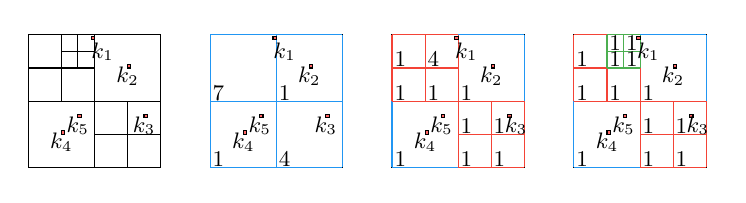
\begin{tikzpicture}[scale=0.21, every node/.style={scale=0.9}]
		
		% \draw[gray, very thin] (0,0) grid +(8,8);
		
		
		\begin{scope}[shift={(0,0)}]
		\draw (0,0) rectangle +(8,8);
		\draw[step=4] (0,0) grid +(8,8);
		\draw[step=2] (0,4) grid +(4,4);
		\draw[step=2] (4,0) grid +(4,4);
		\draw[step=1] (2,6) grid +(2,2);
		
		\draw[fill=red!60] (3.8,7.7) rectangle +(0.2,0.2);
		\node at (4.5,7.0) {\small $k_1$};
		\draw[fill=red!60] (6,6) rectangle +(0.2,0.2);
		\node at (6,5.5) {\small $k_2$};
		\draw[fill=red!60] (7,3) rectangle +(0.2,0.2);
		\node at (7,2.5) {\small $k_3$};
		\draw[fill=red!60] (2,2) rectangle +(0.2,0.2);
		\node at (2.0,1.5) {\small $k_4$};
		\draw[fill=red!60] (3,3) rectangle +(0.2,0.2);
		\node at (3.0,2.5) {\small $k_5$};
		
		\end{scope}	 	
		
		\begin{scope}[shift={(11,0)}]
		\draw (0,0) rectangle +(8,8);
		\draw[step=4,cpu4] (0,0) grid +(8,8);
		
		\node at (0.5,0.5) {\small $1$};
		\node at (4.5,0.5) {\small $4$};
		\node at (0.5,4.5) {\small $7$};
		\node at (4.5,4.5) {\small $1$};
		
		\draw[fill=red!60] (3.8,7.7) rectangle +(0.2,0.2);
		\node at (4.5,7.0) {\small $k_1$};
		\draw[fill=red!60] (6,6) rectangle +(0.2,0.2);
		\node at (6,5.5) {\small $k_2$};
		\draw[fill=red!60] (7,3) rectangle +(0.2,0.2);
		\node at (7,2.5) {\small $k_3$};
		\draw[fill=red!60] (2,2) rectangle +(0.2,0.2);
		\node at (2.0,1.5) {\small $k_4$};
		\draw[fill=red!60] (3,3) rectangle +(0.2,0.2);
		\node at (3.0,2.5) {\small $k_5$};
		
		\end{scope}
		
		\begin{scope}[shift={(22,0)}]
		\draw (0,0) rectangle +(8,8);
		\draw[step=4,cpu4] (0,0) grid +(8,8);
		\draw[step=2,cpu3] (0,4) grid +(4,4);
		\draw[step=2,cpu3] (4,0) grid +(4,4);
		\node at (0.5,0.5) {\small $1$};
		
		\node at (4.5,0.5) {\small $1$};
		\node at (6.5,0.5) {\small $1$};
		\node at (4.5,2.5) {\small $1$};
		\node at (6.5,2.5) {\small $1$};
		
		\node at (0.5,4.5) {\small $1$};
		\node at (2.5,4.5) {\small $1$};
		\node at (0.5,6.5) {\small $1$};
		\node at (2.5,6.5) {\small $4$};
		
		\node at (4.5,4.5) {\small $1$};	
		
		\draw[fill=red!60] (3.8,7.7) rectangle +(0.2,0.2);
		\node at (4.5,7.0) {\small $k_1$};
		\draw[fill=red!60] (6,6) rectangle +(0.2,0.2);
		\node at (6,5.5) {\small $k_2$};
		\draw[fill=red!60] (7,3) rectangle +(0.2,0.2);
		\node at (7.5,2.5) {\small $k_3$};
		\draw[fill=red!60] (2,2) rectangle +(0.2,0.2);
		\node at (2.0,1.5) {\small $k_4$};
		\draw[fill=red!60] (3,3) rectangle +(0.2,0.2);
		\node at (3.0,2.5) {\small $k_5$};
		\end{scope}
		
		\begin{scope}[shift={(33,0)}]
		\draw (0,0) rectangle +(8,8);
		\draw[step=4,cpu4] (0,0) grid +(8,8);
		\draw[step=2,cpu3] (0,4) grid +(4,4);
		\draw[step=2,cpu3] (4,0) grid +(4,4);
		\draw[step=1,cpu1] (2,6) grid +(2,2);
		
		\node at (0.5,0.5) {\small $1$};
		
		\node at (4.5,0.5) {\small $1$};
		\node at (6.5,0.5) {\small $1$};
		\node at (4.5,2.5) {\small $1$};
		\node at (6.5,2.5) {\small $1$};
		
		\node at (0.5,4.5) {\small $1$};
		\node at (2.5,4.5) {\small $1$};
		\node at (0.5,6.5) {\small $1$};
		
		\node at (2.5,6.5) {\small $1$};
		\node at (3.5,6.5) {\small $1$};
		\node at (2.5,7.5) {\small $1$};
		\node at (3.5,7.5) {\small $1$};
		
		\node at (4.5,4.5) {\small $1$};		
		
		
		\draw[fill=red!60] (3.8,7.7) rectangle +(0.2,0.2);
		\node at (4.5,7.0) {\small $k_1$};
		\draw[fill=red!60] (6,6) rectangle +(0.2,0.2);
		\node at (6,5.5) {\small $k_2$};
		\draw[fill=red!60] (7,3) rectangle +(0.2,0.2);
		\node at (7.5,2.5) {\small $k_3$};
		\draw[fill=red!60] (2,2) rectangle +(0.2,0.2);
		\node at (2.0,1.5) {\small $k_4$};
		\draw[fill=red!60] (3,3) rectangle +(0.2,0.2);
		\node at (3.0,2.5) {\small $k_5$};
		
		\end{scope}
		\end{tikzpicture}
	}
	\caption{\label{fig:sfcSearch}\small For a given ordered octree $\tau$  and a set of keys (leftmost figure), \tsearch~ performs the traversal in a top-down order over the set of keys, while flagging $k_2,k_4,k_5$ at the level $1$ split, $k_3$ at level $2$ split, and $k_1$ at level $3$ split. %Note that numbers inside the octants (i.e. bucket count) represent the number of octants in $\tau$ belongs to that bucket at splitting level $l$. When bucket count of octant $e\in \tau$ reaches $1$, all the keys in that bucket flagged as found and $e$ is considered to be the search result for those keys. 
	}
	\vspace{-0.15in}
\end{figure}

\subsection{\unzip~ \& \zip : Finite difference computations on adaptive grids}
\label{sec:unzip_and_zip}
The main objective of the \unzip~ and \zip~ operations is to enable stencil computations on adaptive octrees. Any adaptive octree can be considered as a union of regular sub-octrees which we referred  as blocks or \emph{octree to block decomposition}. To perform stencil computations on these blocks, it is required to have neighborhood region surrounding the block which referred as \emph{padding}. The block with surrounding  padding region is referred as \unzip~ representation(see Figure 6 on the poster). The stencil and other update operations are only performed on the block as the padding is read-only. At the end of the update, the simulation variables are {\em zipped} back, i.e., injected back to the {\em zipped} representation. Note that several key operations such as RK update \& inter-process communications operate using the \textit{zip} representation, and are efficient (see Figure 3 on the poster ).  








%\begin{algorithm}
%	\caption{\small Overview of our approach}\label{alg:overview}
%	\footnotesize
%	\begin{algorithmic}[1]
%		%\Require A list of points or regions $W$, the starting level $l_1$ and the ending level $l_2$, $K_{oct}$
%		%\Ensure $\tau_c$ \- ordered complete octree based on $W$
%		%\Function{TreeSort($W$, $l_1$, $l_2$)}{}
%		\State $M \leftarrow$ initialize mesh \Comment{meshing}
%		\State $u \leftarrow$ initialize variables $(M)$
%		\While{$t < T$}
%		\For{$r = 1:3$} \Comment{Runge-Kutta stages}
%		\State $B, \hat{u} \leftarrow \text{Unzip}(M, u)$ \Comment{\S\ref{sec:unzip_and_zip}}
%		\For{$ b \in B$} 
%		\State Compute derivatives \Comment Machine generated code 
%		\State Compute $\hat{u}_{rhs}(b)$ \Comment Machine generated code 
%		\EndFor % blocks
%		\State $u_{rhs} \leftarrow \text{Zip}(M, B, \hat{u}_{rhs})$ \Comment{\S\ref{sec:unzip_and_zip}}
%		\State RK update
%		\EndFor  % rk 
%		\State $t\leftarrow t+dt$
%		\If{need remesh $M$}  \Comment{remesh }
%		\State $M' \leftarrow$ remesh($M$) 
%		\State $u' \leftarrow$ Intergid\_Transfer$(M, M', u)$ \Comment{inter-grid transfer}
%		\EndIf
%		\EndWhile  % time
%	\end{algorithmic}
%\end{algorithm}


\subsection{Symbolic interface and code generation}
The Einstein equations are a set of non-linear, coupled, partial 
differential equations. On discretization, one can end up with 24 or 
more equations with thousands of terms. Writing, optimizing and maintaining 
code for this is very challenging. Sustainability and keeping it relevant for new 
architectural changes are additional difficulties. To address these issues, we 
have developed a symbolic interface to \dendrogr. We leverage symbolic python 
(\texttt{SymPy}) as the backend for this along with the python package 
\texttt{cog} to embed python code within our application-level \texttt{C++} 
code(see symbolic code generation on the poster).

%The \texttt{\dendro\_sym} package allows us to write the discretized 
%versions of the equations similar to how they are written mathematically 
%and enable improved usability for non-computational scientists. 


%\subsection{Numerical Methods}
%\label{sec:nm}
%In this section we briefly outline our particular choices for 
%solving these equations. We write the \BSSN\ equations in terms of the conformal 
%factor $\chi$. We use the parameterization of the
%``$1+\log$'' slicing condition and the $\Gamma$-driver shift.
%Spatial derivatives are calculated using finite difference operators that are ${\rm O}(h^4)$ in the grid spacing, $h$, 
%with upwind derivatives for some Lie derivative terms. 
%%We calculate derivatives for the Ricci tensor and enforce the algebraic
%%constraints as described in~\cite{Bruegmann:2006at}. 
%Outgoing radiative boundary conditions are applied to each \BSSN\ function.
%The BSSN equations are integrated in time using an explicit Runge-Kutta (RK)
%scheme. The solution at each point is integrated
%with a single global times step, that is set by the smallest grid spacing
%and the Courant condition.
%The tests in this paper were done 
%using third order RK with Courant factor $\lambda=0.1$. 
%Kreiss-Oliger dissipation is added~\cite{kodissipation,Alcubierre:1138167} 
%to the solution to eliminate high-frequency noise that can be generated 
%near the black hole singularities.



%\begin{figure}[H]
%	\centering
%	\resizebox{0.4\textwidth}{!}{
%		\begin{tikzpicture}[scale=0.2,every node/.style={scale=0.6}]
%		
%		\begin{scope}[shift={(0,0)}]
%		\draw[step=5cm] (0,0) grid +(10,10);
%		\draw[step=2.5cm] (5,0) grid +(5,5);
%		\draw[step=2.5cm] (0,5) grid +(5,5);
%		
%		\def \r{0.12}
%		\foreach \x in {0,2.5,5}{
%			\foreach \y in {0,2.5,5}{
%				\draw[red,fill=red] (\x,\y) circle (\r);
%			}
%		}
%		
%		\foreach \x in {5,7.5,10}{
%			\foreach \y in {5,7.5,10}{
%				\draw[red,fill=red] (\x,\y) circle (\r);
%			}
%		}
%		
%		\foreach \x in {0,1.25,2.5,3.75}{
%			\foreach \y in {6.25,7.5,8.75,10}{
%				\draw[blue,fill=blue] (\x,\y) circle (\r);
%			}
%		}	
%		
%		\foreach \x in {6.25,7.5,8.75,10}{
%			\foreach \y in {0,1.25,2.5,3.75}{
%				\draw[blue,fill=blue] (\x,\y) circle (\r);
%			}
%		}
%		\end{scope}
%		
%		\begin{scope}[shift={(14,0)}]
%		%\draw[cyan,thick,fill=blue!20] (-1,-1) rectangle +(6,6);
%		\draw[cyan,thick] (0,0) rectangle +(5,5);
%		\draw[cyan,thick,xshift=2cm,yshift=2.0cm] (5,5) rectangle +(5,5);
%		\draw[cyan,thick,step=2.5cm,xshift=2.0cm] (5,0) grid +(5,5);
%		\draw[cyan,thick,step=2.5cm,yshift=2.0cm] (0,5) grid +(5,5);
%		%	\draw[cyan,thick] (0,4) rectangle +(2,2);
%		%	\draw[cyan,thick] (2,4) rectangle +(2,2);
%		%	\draw[cyan,thick] (2,6) rectangle +(2,2);
%		%	\draw[cyan,thick] (4,0) rectangle +(2,2);
%		%	\draw[cyan,thick] (6,2) rectangle +(2,2);
%		%	\draw[cyan,thick] (6,0) rectangle +(2,2);
%		\end{scope}
%		
%		\begin{scope}[shift={(30,0)}]
%		\def \r{0.12}
%		\draw[cyan,fill=blue!50,fill opacity=0.5]
%		(-2,-2)--(-2,6)--(6,6)--(6,-2)--cycle
%		(0,0) -- (4,0)-- (4,4)--(0,4)--cycle;
%		\foreach \x in {-2,0,2,2,4,6}{
%			\foreach \y in {-2,0,2,2,4,6}{
%				\draw[red,fill=red] (\x,\y) circle (\r);
%			}
%		}
%		
%		\draw[cyan,thick,fill=blue!50,fill opacity=0.5,even odd rule,xshift=8.5cm,yshift=8.5cm] 
%		(-2,-2)--(-2,6)--(6,6)--(6,-2)--cycle
%		(0,0) -- (4,0)-- (4,4)--(0,4)--cycle;
%		\foreach \x in {-2,0,2,2,4,6}{
%			\foreach \y in {-2,0,2,2,4,6}{
%				\draw[red,fill=red,xshift=8.5cm,yshift=8.5cm] (\x,\y) circle (\r);
%			}
%		}
%		
%		\draw[cyan,thick,fill=blue!50,fill opacity=0.5,even odd rule,xshift=8.5cm] 
%		(-1,-1)--(-1,5)--(5,5)--(5,-1)--cycle
%		(0,0) -- (4,0)-- (4,4)--(0,4)--cycle;
%		\draw[cyan,thick,step=2,xshift=8.5cm] (0,0) grid +(4,4);
%		\foreach \x in {-1,0,1,2,3,4,5}{
%			\foreach \y in {-1,0,1,2,3,4,5}{
%				\draw[blue,fill=blue,xshift=8.5cm] (\x,\y) circle (\r);
%			}
%		}
%		
%		\draw[cyan,thick,fill=blue!50,fill opacity=0.5,even odd rule,yshift=8.5cm] 
%		(-1,-1)--(-1,5)--(5,5)--(5,-1)--cycle
%		(0,0) -- (4,0)-- (4,4)--(0,4)--cycle;
%		\draw[cyan,thick,step=2,yshift=8.5cm] (0,0) grid +(4,4);	
%		\foreach \x in {-1,0,1,2,3,4,5}{
%			\foreach \y in {-1,0,1,2,3,4,5}{
%				\draw[blue,fill=blue,yshift=8.5cm] (\x,\y) circle (\r);
%			}
%		}
%		
%		\end{scope}	
%		\end{tikzpicture}
%	}	
%	\caption{\label{fig:unzip} \small A simplistic example of octree to block decomposition and \unzip~ operation. The leftmost figure shows the considering adaptive octree with \textit{zip} state and its block decomposition is shown in the middle. The rightmost figure shows the decomposed blocks padded with values coming from neighboring octants with interpolation if needed.}
%	\vspace{-0.15in}
%\end{figure}

%\subsection{Putting everything together}
%
%We use a $3^{rd}$ order Runge-Kutta time stepper, to perform time evolution.  A given RK stage is computed by performing \unzip ~ operations with overlapped exchange of the ghost layer for the evolution variables, computation of the derivatives and right-hand-side (rhs) (using the code generated by the symbolic framework) for all local blocks and finally performing \zip~ operation to get the computed {\em zipped} rhs variables. The RK update is then performed on the {\em zipped} variables. An complete outline of our approach for simulating binary BH mergers demonstrating how the various components come together is listed in Algorithm \ref{alg:overview} and illustrated in Figure \ref{fig:overview}.
\vspace{-0.15in}
\section{Results}
In this section, we present results on scalability studies performed on \dendrogr~ (see Figures \ref{fig:ss_r10} \& \ref{fig:ws_g1000}) and comparison study with the \ET (see Figure \ref{fig:et_sans_adaptivity}) which also provides an insight on the efficiency of WAMR grid compared to structured/block adaptivity. We also present a comparison study between \tsearch~ \& binary search approach (see Figure 5 on the poster ). 

%\begin{figure}[tbh]
%	\centering
%	\begin{tikzpicture}
%	\begin{axis}[legend pos= north west,xlabel={number of keys $\rightarrow$},symbolic x coords={100,1K,10K,100K,1M,10M,20M,33M,64M},
%	xtick={data},
%	ylabel={time(s) $\rightarrow$},grid=major,width=9cm,height=4cm]
%	\addplot [sq_b1,thin,mark=*]table [x={numKeys},y={bsearch_time_s}]{dat/stampede2/tsearch.dat};
%	\addplot [sq_r1,thin,mark=x] table [x={numKeys},y={tsearch_time_s}]{dat/stampede2/tsearch.dat};
%	\legend{\texttt{std::bsearch}, \tsearch }
%	\end{axis}
%	\end{tikzpicture}
%	\caption{Comparison of \texttt{std::bsearch} with partial ordering operator $<$ and comparison free \tsearch~ approach for performing, varying number of keys on $33M$ sorted complete octree using single core in \Stampede~ \texttt{SKX} node.}
%	\label{fig::balcomparison}
%\end{figure}

\begin{figure}[tbh]
	\centering
	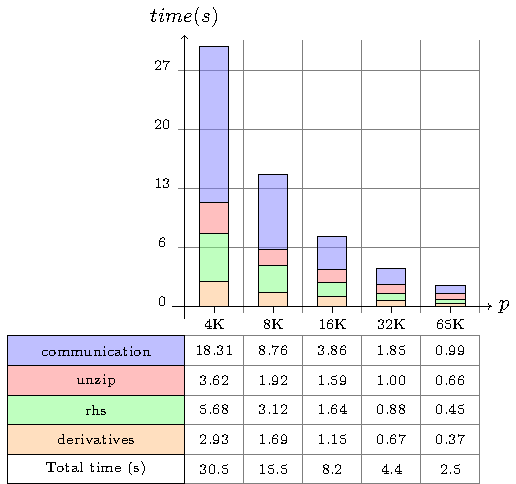
\includegraphics[width=0.3\textwidth]{plots/strong_r10}
	\caption{\small Strong scaling results in ORNL's \Titan~for a single RK step (averaged over 10 steps) with derivative computation (\texttt{deriv}), right hand side( {\texttt rhs}) computation, \texttt{unzip} cost 
		and communication cost (\texttt{comm}) for a fixed problem size of $10.5B$ unknowns where the number of cores ranging from $4,096$ to $65,536$ cores on $4096$ nodes. Note that for strong scaling results re-meshing is disabled in order to keep the problem size fixed.  \label{fig:ss_r10} }
	\vspace{-0.2in}
\end{figure}

\begin{figure}[tbh]
	\centering
	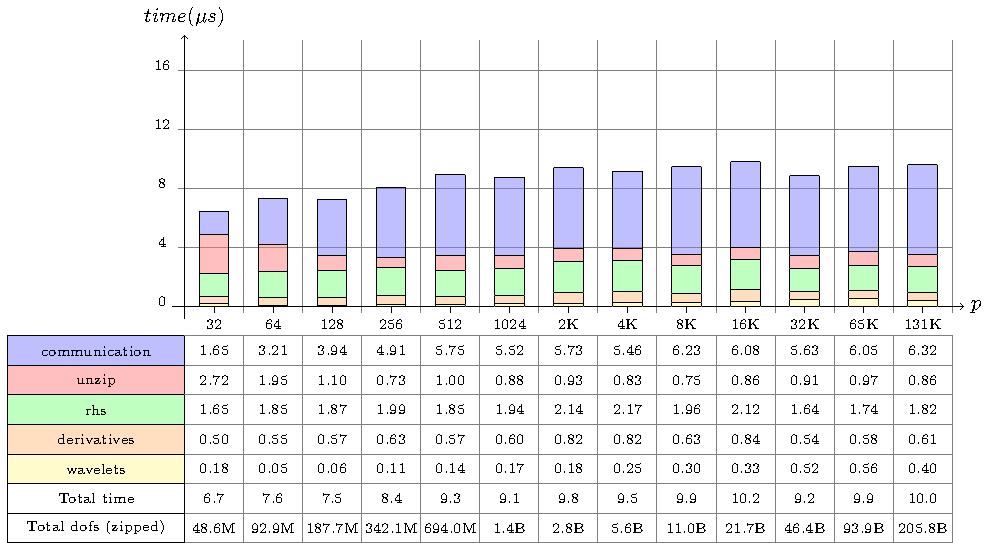
\includegraphics[width=0.8\columnwidth]{plots/weak_r10}
	\caption{\small Weak scaling results in ORNL's \Titan~for  $RK/(dof/p)$ (averaged over 10 steps) where $RK,dof,p$ denotes the time for single $RK$ step, degrees of freedom, and number of cores respectively, where the approximate grain size of 1.536M unknowns where the number of cores ranging from $32$ to $131,072$ cores on $8192$ nodes where the largest problem having $206$ Billion unknowns. \label{fig:ws_g1000} 
		%Above results are generated with mass ratio $\mu=10$ with \maxDepth~ 18 and wavelet tolerance of $10^{-6}$ \label{fig:ws_g1000} 
	}
	\vspace{-0.1in}
\end{figure}

\begin{figure}[tbh]
  \centering
\resizebox{0.9\columnwidth}{!}{
	\begin{tikzpicture}[scale=0.8]
	\begin{axis}[
	ylabel={time per $RK$ step (s) $\rightarrow$},
	% xlabel={number of cores $\rightarrow$},
	legend pos=north west,symbolic x coords={48,96,192,384,768,1536,3072},xtick = data,
	height=3.38in,
	width=3.38in,
	%extra x tick style={tick label style={black, below, yshift=1.5ex}},
	xticklabels=\empty,
	ticklabel style={left}, grid=major, 
	extra x ticks={48,96,192,384,768,1536,3072},
	extra x tick labels={48,96,192,384,768,1536,3072},
	extra x tick style={tick label style={black, below, yshift=0.5ex}},
	legend style={at={(0.5,1.05)},anchor=south},
	%yticklabels=\empty,
	%extra y tick style={yticklabel style={xshift=1cm, anchor=west}}
	]
	\addplot[thick,sq_b1,smooth,mark options={scale=0.8}]  table [x={npes},y ={rkstep}]{dat/stampede2/et_ss_4M.dat};
	\addplot[thick,sq_g1,smooth,mark options={scale=0.8}]  table [x={npes},y ={rkstep}]{dat/stampede2/dendro_ss_4M.dat};
	
	\addplot[thick,sq_b2,opacity=0.6,smooth]  table [x={npes},y ={rkstep_ws_3}]{dat/stampede2/et_ws_2K.dat};
	\addplot[thick,sq_g2,opacity=0.6,smooth]  table [x={npes},y ={rkstep_ws_3}]{dat/stampede2/dendro_ws_2K.dat};
	\legend{\small \ET(strong scaling), \dendrogr(strong scaling), \ET(weak scaling), \dendrogr(weak scaling) }
	
	\end{axis}
	
	\begin{scope}[xshift=-2.5cm]
	% dendro
	%table grid
	\draw (-7,0) grid +(7,7);
	% weak scaling highlight
	\draw[fill=sq_g1, opacity=0.3] (-6-1,0) rectangle +(1,1);
	\draw[fill=sq_g1, opacity=0.3] (-5-1,1) rectangle +(1,1);
	\draw[fill=sq_g1, opacity=0.3] (-4-1,2) rectangle +(1,1);
	\draw[fill=sq_g1, opacity=0.3] (-3-1,3) rectangle +(1,1);
	\draw[fill=sq_g1, opacity=0.3] (-2-1,4) rectangle +(1,1);
	\draw[fill=sq_g1, opacity=0.3] (-1-1,5) rectangle +(1,1);
	\draw[fill=sq_g1, opacity=0.3] (-1,6) rectangle +(1,1);
	
	% strong scaling highlight
	\draw[fill=sq_g1, opacity=0.5, sq_g1] (-6.01-1,3) rectangle +(6.02+1,1);
	
	% data - dendro
	%                 48                                       96                                          192                                           384                                768                                 1536	3072
	\node at (-5.5-1,0.5) {\scriptsize $0.83$}; \node at (-4.5-1,0.5) {\scriptsize $0.55$}; \node at (-3.5-1,0.5) {\scriptsize $0.37$}; \node at (-2.5-1,0.5) {\scriptsize $-$}; \node at (-1.5-1,0.5) {\scriptsize $-$}; \node at (-0.5-1,0.5) {\scriptsize $-$}; \node at (-0.5,0.5) {\scriptsize $-$}; % 500K
	\node at (-5.5-1,1.5) {\scriptsize $1.58$}; \node at (-4.5-1,1.5) {\scriptsize $0.86$}; \node at (-3.5-1,1.5) {\scriptsize $0.51$}; \node at (-2.5-1,1.5) {\scriptsize $0.35$}; \node at (-1.5-1,1.5) {\scriptsize $-$}; \node at (-0.5-1,1.5) {\scriptsize $-$};  \node at (-0.5,1.5) {\scriptsize $-$};% 1M
	\node at (-5.5-1,2.5) {\scriptsize $2.98$}; \node at (-4.5-1,2.5) {\scriptsize $1.57$}; \node at (-3.5-1,2.5) {\scriptsize $0.83$}; \node at (-2.5-1,2.5) {\scriptsize $0.61$}; \node at (-1.5-1,2.5) {\scriptsize $0.38$}; \node at (-0.5-1,2.5) {\scriptsize $-$}; \node at (-0.5,2.5) {\scriptsize $-$};% 2M
	\node at (-5.5-1,3.5) {\scriptsize $5.90$};    \node at (-4.5-1,3.5) {\scriptsize $3.35$}; \node at (-3.5-1,3.5) {\scriptsize $1.75$}; \node at (-2.5-1,3.5) {\scriptsize $1.04$}; \node at (-1.5-1,3.5) {\scriptsize $0.54$}; \node at (-0.5-1,3.5) {\scriptsize $0.39$}; \node at (-0.5,3.5) {\scriptsize $-$}; % 4M
	\node at (-5.5-1,4.5) {\scriptsize $11.23$};    \node at (-4.5-1,4.5) {\scriptsize $6.59$};    \node at (-3.5-1,4.5) {\scriptsize $3.67$}; \node at (-2.5-1,4.5) {\scriptsize $1.92$}; \node at (-1.5-1,4.5) {\scriptsize $1.10$}; \node at (-0.5-1,4.5) {\scriptsize $0.69$}; \node at (-0.5,4.5) {\scriptsize $0.38$};% 8M
	\node at (-5.5-1,5.5) {\scriptsize $19.22$};    \node at (-4.5-1,5.5) {\scriptsize $11.08$};    \node at (-3.5-1,5.5) {\scriptsize $6.22$};    \node at (-2.5-1,5.5) {\scriptsize $3.20$}; \node at (-1.5-1,5.5) {\scriptsize $1.64$}; \node at (-0.5-1,5.5) {\scriptsize $0.98$}; \node at (-0.5,5.5) {\scriptsize $0.56$};% 16M
	\node at (-5.5-1,6.5) {\scriptsize $35.46$};    \node at (-4.5-1,6.5) {\scriptsize $-$};    \node at (-3.5-1,6.5) {\scriptsize $12.34$};    \node at (-2.5-1,6.5) {\scriptsize $6.88$};    \node at (-1.5-1,6.5) {\scriptsize $4.01$}; \node at (-0.5-1,6.5) {\scriptsize $2.06$};  \node at (-0.5,6.5) {\scriptsize $1.06$};% 32M
	
	\node at (-5.5-1,-0.25) {\scriptsize $48$};
	\node at (-4.5-1,-0.25) {\scriptsize $96$};
	\node at (-3.5-1,-0.25) {\scriptsize $192$};
	\node at (-2.5-1,-0.25) {\scriptsize $384$};
	\node at (-1.5-1,-0.25) {\scriptsize $768$};
	\node at (-0.5-1,-0.25) {\scriptsize $1536$};
	\node at (-0.5,-0.25)   {\scriptsize $3072$};
	
	
	\draw[-latex'] (-6.25-1,6.75) -- (-6.25-1,7.25); \node at (-6.75-1, 7) {\scriptsize dofs};  \node at (-6.75-1, 7.35) {\scriptsize total};
	
	\node at (-6.6-1,6.5) {\scriptsize $768M$};
	\node at (-6.6-1,5.5) {\scriptsize $384M$};
	\node at (-6.6-1,4.5) {\scriptsize $192M$};
	\node at (-6.6-1,3.5) {\scriptsize $96M$};
	\node at (-6.6-1,2.5) {\scriptsize $48M$};
	\node at (-6.6-1,1.5) {\scriptsize $24M$};
	\node at (-6.6-1,0.5) {\scriptsize $12M$};
	
	\draw[-latex'] (0,-0.25) -- (0.75,-0.25); \node at (1.0, 0) {\scriptsize cores};
	
	\draw[-latex'] (-1,7.3) -- (-1,7.8);   \node at (0, 7.5) {\scriptsize per core};  \node at (0, 8) {\scriptsize dofs (along the diagonal) };    
	
	\draw[-latex'] (0.25,7.25) -- (-0.25,6.75); \node at (0.75,7) {\scriptsize $250K$};
	\draw[-latex'] (0.25,6.25) -- (-0.25,5.75); \node at (0.75,6) {\scriptsize $125K$};
	\draw[-latex'] (0.25,5.25) -- (-0.25,4.75); \node at (0.75,5) {\scriptsize $62K$};
	\draw[-latex'] (0.25,4.25) -- (-0.25,3.75); \node at (0.75,4) {\scriptsize $31K$};
	\draw[-latex'] (0.25,3.25) -- (-0.25,2.75); \node at (0.75,3) {\scriptsize $15K$};
	\draw[-latex'] (0.25,2.25) -- (-0.25,1.75); \node at (0.75,2) {\scriptsize $8K$};
	\draw[-latex'] (0.25,1.25) -- (-0.25,0.75); \node at (0.75,1) {\scriptsize $4K$};
	
	\node at (-4, 9) {\dendrogr};
	
	
	
	\end{scope}
	
	\begin{scope}[xshift=2.5cm]
	% ET
	% table grid
	\draw (7,0) grid +(7,7);
	% weak highlight 
	\draw[fill=sq_b1, opacity=0.3] (7,0) rectangle +(1,1);
	\draw[fill=sq_b1, opacity=0.3] (8,1) rectangle +(1,1);
	\draw[fill=sq_b1, opacity=0.3] (9,2) rectangle +(1,1);
	\draw[fill=sq_b1, opacity=0.3] (10,3) rectangle +(1,1);
	\draw[fill=sq_b1, opacity=0.3] (11,4) rectangle +(1,1);
	\draw[fill=sq_b1, opacity=0.3] (12,5) rectangle +(1,1);
	\draw[fill=sq_b1, opacity=0.3] (12,5) rectangle +(1,1);
	
	%strong highlights 
	\draw[fill=sq_b1, opacity=0.5, sq_b1] (6.99,3) rectangle +(6.02+1,1);
	
	% data - ET 
	%                 48                                       96                                          192                                           384                                768                                 1536 
	\node at (7.5,0.5) {\scriptsize $2.27$}; \node at (8.5,0.5) {\scriptsize $2.06$}; \node at (9.5,0.5) {\scriptsize $1.93$}; \node at (10.5,0.5) {\scriptsize $1.88$}; \node at (11.5,0.5) {\scriptsize $2.03$}; \node at (12.5,0.5) {\scriptsize $2.07$}; \node at (13.5,0.5) {\scriptsize $-$};% 500K
	\node at (7.5,1.5) {\scriptsize $2.67$}; \node at (8.5,1.5) {\scriptsize $2.31$}; \node at (9.5,1.5) {\scriptsize $2.08$}; \node at (10.5,1.5) {\scriptsize $1.94$}; \node at (11.5,1.5) {\scriptsize $2.07$}; \node at (12.5,1.5) {\scriptsize $2.04$}; \node at (13.5,1.5) {\scriptsize $-$}; % 1M
	\node at (7.5,2.5) {\scriptsize $3.36$}; \node at (8.5,2.5) {\scriptsize $2.68$}; \node at (9.5,2.5) {\scriptsize $2.31$}; \node at (10.5,2.5) {\scriptsize $2.08$}; \node at (11.5,2.5) {\scriptsize $2.12$}; \node at (12.5,2.5) {\scriptsize $2.08$}; \node at (13.5,2.5) {\scriptsize $-$};% 2M
	\node at (7.5,3.5) {\scriptsize $4.68$};    \node at (8.5,3.5) {\scriptsize $3.46$}; \node at (9.5,3.5) {\scriptsize $2.69$}; \node at (10.5,3.5) {\scriptsize $2.32$}; \node at (11.5,3.5) {\scriptsize $3.45$}; \node at (12.5,3.5) {\scriptsize $2.16$}; \node at (13.5,3.5) {\scriptsize $-$}; % 4M
	\node at (7.5,4.5) {\scriptsize $7.13$};    \node at (8.5,4.5) {\scriptsize $4.76$};    \node at (9.5,4.5) {\scriptsize $3.45$}; \node at (10.5,4.5) {\scriptsize $2.74$}; \node at (11.5,4.5) {\scriptsize $2.51$}; \node at (12.5,4.5) {\scriptsize $2.31$}; \node at (13.5,4.5) {\scriptsize $-$}; % 8M
	\node at (7.5,5.5) {\scriptsize $12.44$};    \node at (8.5,5.5) {\scriptsize $7.51$};    \node at (9.5,5.5) {\scriptsize $4.87$};    \node at (10.5,5.5) {\scriptsize $3.48$}; \node at (11.5,5.5) {\scriptsize $2.92$}; \node at (12.5,5.5) {\scriptsize $2.52$}; \node at (13.5,5.5) {\scriptsize $-$};% 16M
	\node at (7.5,6.5) {\scriptsize $23.38$};    \node at (8.5,6.5) {\scriptsize $12.65$};    \node at (9.5,6.5) {\scriptsize $7.64$};    \node at (10.5,6.5) {\scriptsize $4.93$};    \node at (11.5,6.5) {\scriptsize $3.71$}; \node at (12.5,6.5) {\scriptsize $2.95$}; \node at (13.5,6.5) {\scriptsize $-$};% 32M    
	
	\node at (7.5,-0.25) {\scriptsize $48$};
	\node at (8.5,-0.25) {\scriptsize $96$};
	\node at (9.5,-0.25) {\scriptsize $192$};
	\node at (10.5,-0.25) {\scriptsize $384$};
	\node at (11.5,-0.25) {\scriptsize $768$};
	\node at (12.5,-0.25) {\scriptsize $1536$};
	\node at (13.5,-0.25) {\scriptsize $3072$};
	
	\draw[-latex'] (13+1,-0.25) -- (14+1,-0.25); \node at (13.5+1, 0) {\scriptsize cores};
	
	\draw[-latex'] (6.75,6.75) -- (6.75,7.25); \node at (6.25, 7) {\scriptsize dofs};  \node at (6.25, 7.35) {\scriptsize total};
	
	\node at (7.25-1,6.5) {\scriptsize $768M$};
	\node at (7.25-1,5.5) {\scriptsize $384M$};
	\node at (7.25-1,4.5) {\scriptsize $192M$};
	\node at (7.25-1,3.5) {\scriptsize $96M$};
	\node at (7.25-1,2.5) {\scriptsize $48M$};
	\node at (7.25-1,1.5) {\scriptsize $24M$};
	\node at (7.25-1,0.5) {\scriptsize $12M$};
	
	
	\draw[-latex'] (14,7.3) -- (14,7.8);   \node at (13+2.25, 7.5) {\scriptsize per core};  \node at (13+2.25, 8) {\scriptsize dofs (along the diagonal) };    
	%\node at (13.4, 7) {\scriptsize size};  \node at (13.5, 7.35) {\scriptsize grain};
	
	\draw[-latex'] (13.25+1,7.25) -- (12.75+1,6.75); \node at (13.75+1,7) {\scriptsize $250K$};
	\draw[-latex'] (13.25+1,6.25) -- (12.75+1,5.75); \node at (13.75+1,6) {\scriptsize $125K$};
	\draw[-latex'] (13.25+1,5.25) -- (12.75+1,4.75); \node at (13.75+1,5) {\scriptsize $62K$};
	\draw[-latex'] (13.25+1,4.25) -- (12.75+1,3.75); \node at (13.75+1,4) {\scriptsize $31K$};
	\draw[-latex'] (13.25+1,3.25) -- (12.75+1,2.75); \node at (13.75+1,3) {\scriptsize $15K$};
	\draw[-latex'] (13.25+1,2.25) -- (12.75+1,1.75); \node at (13.75+1,2) {\scriptsize $8K$};
	\draw[-latex'] (13.25+1,1.25) -- (12.75+1,0.75); \node at (13.75+1,1) {\scriptsize $4K$};
	
	\node at (11, 9) {\ET};
	
	
	\end{scope}
	
	
	
	
	
	% table 
	
	
	
	% axis
	%\node at (axis cs:64,11) [anchor=north west] {\tiny $48M$};
	
	
		
	
	
	
	\end{tikzpicture}
}
\caption{\label{fig:et_sans_adaptivity} \small Comparison between \ET~ and \dendrogr\ without factoring in adaptivity (i.e. both \ET~ \& \dendrogr~ support uniform grids.). For a fixed tolerance, we expand the domain for a $1:1$ mass-ratio simulation such that both \ET~ and \dendrogr\ have roughly the same number of dofs. We present both weak and strong scaling results using both codes. On the left table are results from \dendrogr\ and from \ET\  on the right. In the middle, we plot a representative strong and weak scaling curve for each code. The \dendrogr\  scaling is plotted in green (lighter shade for weak) and blue for \ET. The corresponding data entries are also marked in the tables. Note that the rows represent strong scaling and the diagonal entries represent weak scaling results and runtime is reported in seconds$(s)$. }
\vspace{-0.2in}
\end{figure}













%============ Conclusion ===============
%\section{Conclusion}

%In the short time that LIGO and Virgo
%have been searching for
%gravitational waves, we have already learned exciting things about
%neutron stars~\cite{Most:2018hfd,Shibata:2017xdx}, 
%the production of heavy elements 
%(such as gold)~\cite{0004-637X-855-2-99}, 
%and the population of black holes in the 
%universe~\cite{TheLIGOScientific:2016htt}. 
%When gravitational wave observations are combined with observations of
%electromagnetic radiation---from radio waves to gamma rays---there is
%a multiplicative effect that magnifies the scientific impact. This is
%the promise of multi-messenger astronomy.
%
%The full scientific
%impact of multi-messenger astronomy is only realized when the
%observations are informed by sophisticated computer models of the underlying
%astrophysical phenomena. 
%\dendro\ provides the ability to run these models in a scalable way, 
%with local adaptivity criteria using WAMR.
%While AMR codes with block-adaptivity typically lose performance as the number
%of adaptive levels increases, \dendro\ achieves impressive scalability on a real 
%application even with many levels of refinement. The combination of scalability
%and adaptivity will allow us to study the gravitational radiation from
%IMRIs without simplifying approximations in direct numerical simulations.
%
%The \dendro\ code reported on here, with 
%a module for vacuum black hole spacetimes, is just our initial step in 
%creating a highly adaptive computational platform for studying
%relativistic astrophysics on the next-generation of supercomputers.
%This work will be followed with additional modules for solving the
%relativistic magnetohydrodynamics equations, 
%nuclear equations of state, and radiation hydrodynamics.
%For application developers, a key advantage of \dendro\ is the ability to use
%conventional numerical methods for these modules.
%
%As LIGO and Virgo are joined by other gravitational wave detectors and
%observatories around the world, we expect many more exciting 
%discoveries to come.




% conference papers do not normally have an appendix


% use section* for acknowledgement
%\section*{Acknowledgment}
%The authors would like to thank...
%more thanks here
% trigger a \newpage just before the given reference
% number - used to balance the columns on the last page
% adjust value as needed - may need to be readjusted if
% the document is modified later
%\IEEEtriggeratref{8}
% The "triggered" command can be changed if desired:
%\IEEEtriggercmd{\enlargethispage{-5in}}

% references section
%\IEEEtriggeratref{70}
% can use a bibliography generated by BibTeX as a .bbl file
% BibTeX documentation can be easily obtained at:
% http://www.ctan.org/tex-archive/biblio/bibtex/contrib/doc/
% The IEEEtran BibTeX style support page is at:
% http://www.michaelshell.org/tex/ieeetran/bibtex/
\bibliographystyle{IEEEtran}
\bibliography{bssn}


%\newpage
%\pagebreak
%\setcounter{page}{1}
%%\appendix
%\appendices
%
%\section{Artifact Description}
%\label{sec:AD}
%\subsection{Getting and Compiling \dendro~}

The \dendro\ simulation code is freely available at GitHub (\href{https://github.com/paralab/Dendro-GR}{https://github.com/paralab/Dendro-GR}) under the MIT License. 
The latest version of the code can be obtained by cloning the repository
\begin{lstlisting}[basicstyle=\small,language=bash]
$ git clone git@github.com:paralab/Dendro-GR.git
\end{lstlisting}

The following dependencies are required to compile \dendro~
\begin{itemize}
	\item C/C++ compilers with C++11 standards and OpenMP support
	\item MPI implementation (e.g. openmpi, mvapich2 )
	\item ZLib compression library (used to write \texttt{.vtu} files in binary format with compression enabled)
	\item BLAS and LAPACK are optional and not needed for current version of \dendro~
	\item CMake 2.8 or higher version
\end{itemize}

\textbf{Note}: We have tested the compilation and execution of \dendro\ with \texttt{intel}, \texttt{gcc} 4.8 or higher, \texttt{openmpi}, \texttt{mpich2} and \texttt{intelmpi} and \texttt{craympi} (in \Titan) using the linux operating systems. 

To compile the code, execute these commands
\begin{lstlisting}[language=bash]
$ cd <path to DENDRO directory >
$ mkdir build
$ cd build
$ ccmake ../     
\end{lstlisting}
The following options for \dendro\  can then be set in cmake:
\begin{itemize}
	\item \texttt{DENDRO\_COMPUTE\_CONSTRAINTS} : Enables the computation of Hamiltonian and momentum constraints
	\item \texttt{DENDRO\_CONSEC\_COMM\_SELECT}  : If \texttt{ON} sub-communicators are selected from consecrative global ranks, otherwise sub-communicators are selected complete binary tree of global ranks (note that in this case global communicator size need to a power of 2).
	\item \texttt{DENDRO\_ENABLE\_VTU\_CONSTRAINT\_OUT} : Enables constraint variable output \linebreak while time-stepping 
	\item \texttt{DENDRO\_ENABLE\_VTU\_OUTPUT} : Enables evolution variable output while time-stepping
	\item \texttt{DENDRO\_VTK\_BINARY} : If \texttt{ON} vtu files are written in binary format, else ASCII format (binary format recommended).
	\item \texttt{DENDRO\_VTK\_ZLIB\_COMPRES} : If \texttt{ON} binary format is compressed (only effective if \texttt{DENDRO\_VTK\_BINARY} is \texttt{ON})
	\item \texttt{HILBERT\_ORDERING} : Hilbert SFC used if \texttt{ON}, otherwise Morton curve is used. (Hilbert curve is recommended to reduce the communication cost.)
	\item \texttt{NUM\_NPES\_THRESHOLD} : When running in large scale set this to $\sqrt{p}$ where $p$ number of mpi tasks for better performance.
	\item \texttt{RK\_SOLVER\_OVERLAP\_COMM\_AND\_COM} : If \texttt{ON} non blocking communication is used and enable overlapping of communication and computation \textit{unzip} (recommended option), otherwise blocking synchronized \textit{unzip} is used.  	
\end{itemize}

After configuring \dendro, generate the Makefile (use \texttt{c} to configure and \texttt{g} to generate). Then execute \texttt{make all} to build all the targets.  On completion, \bsolver~will be the main executable as related to this paper. 

\subsection{Getting Started: Running \bsolver}

\bsolver\  can be run as follows. 
\begin{lstlisting}[language=bash]
$ mpirun -np <number of mpi tasks>\
 ./bssnSolver \
<parameter file name>.par
\end{lstlisting}
Example parameter files can be found in \texttt{BSSN\_GR/pars/}. The following 
is an example parameter file for equal mass ratio binary inspirals. 
\begin{lstlisting}[basicstyle=\tiny]
	{
	"DENDRO_VERSION": 5.0,
	"BSSN_RESTORE_SOLVER":0,
	"BSSN_IO_OUTPUT_FREQ": 10,
	"BSSN_REMESH_TEST_FREQ": 5,
	"BSSN_CHECKPT_FREQ": 50,
	"BSSN_VTU_FILE_PREFIX": "bssn_gr",
	"BSSN_CHKPT_FILE_PREFIX": "bssn_cp",
	"BSSN_PROFILE_FILE_PREFIX": "bssn_r1",
	"BSSN_DENDRO_GRAIN_SZ": 100,
	"BSSN_ASYNC_COMM_K": 4,
	"BSSN_DENDRO_AMR_FAC": 1e0,
	"BSSN_WAVELET_TOL": 1e-4,
	"BSSN_LOAD_IMB_TOL": 1e-1,
	"BSSN_RK_TIME_BEGIN": 0,
	"BSSN_RK_TIME_END": 1000,
	"BSSN_RK_TIME_STEP_SIZE": 0.01,
	"BSSN_DIM": 3,
	"BSSN_MAXDEPTH": 12,
	"ETA_CONST": 2.0,
	"ETA_R0": 30.0,
	"ETA_DAMPING": 1.0,
	"ETA_DAMPING_EXP": 1.0,
	"BSSN_LAMBDA": {
	"BSSN_LAMBDA_1": 1,
	"BSSN_LAMBDA_2": 1,
	"BSSN_LAMBDA_3": 1,
	"BSSN_LAMBDA_4": 1
	},
	"BSSN_LAMBDA_F": {
	"BSSN_LAMBDA_F0": 1.0,
	"BSSN_LAMBDA_F1": 0.0
	},
	"CHI_FLOOR": 1e-4,
	"BSSN_TRK0": 0.0,
	"KO_DISS_SIGMA": 1e-1,
	"BSSN_BH1": {
	"MASS":0.48528137423856954,
	"X": 4.00000000e+00,
	"Y":0.0,
	"Z": 1.41421356e-05,
	"V_X": -0.00132697,
	"V_Y": 0.1123844,
	"V_Z": 0,
	"SPIN": 0,
	"SPIN_THETA":0,
	"SPIN_PHI": 0
	},
	"BSSN_BH2": {
	"MASS":0.48528137423856954,
	"X":-4.00000000e+00,
	"Y":0.0,
	"Z":1.41421356e-05,
	"V_X": 0.00132697,
	"V_Y": -0.1123844,
	"V_Z": 0,
	"SPIN": 0,
	"SPIN_THETA":0,
	"SPIN_PHI": 0
	}
	}
\end{lstlisting}
Here we list the key options for \bsolver\ with a short description.
\begin{itemize}
\item \texttt{BSSN\_RESTORE\_SOLVER} : Set $1$ to restore $RK$ solver from latest checkpoint. 
\item \texttt{BSSN\_IO\_OUTPUT\_FREQ} : IO (i.e. \texttt{vtu} files) output frequency
\item \texttt{BSSN\_CHECKPT\_FREQ} : Checkpoint file output frequency
\item \texttt{BSSN\_REMESH\_TEST\_FREQ} : Remesh test frequency (i.e. frequency in time steps that is being tested for re-meshing) 
\item \texttt{BSSN\_DENDRO\_GRAIN\_SZ} : Number of octants per core 
\item \texttt{BSSN\_ASYNC\_COMM\_K} : Number of variables that are being processed during an asynchronous \textit{unzip} ($<24$)
\item \texttt{BSSN\_DENDRO\_AMR\_FAC} : Safety factor for coarsening i.e. coarsen if and only if $W_c \leq AMR\_FAC \times WAVELET\_TOL$ where $W_c$ is the computed wavelet coefficient.  
\item \texttt{BSSN\_WAVELET\_TOL} : Wavelet tolerance for WAMR. 
\item \texttt{BSSN\_MAXDEPTH} : Maximum level of refinement allowed ($\leq 30$)
\item \texttt{KO\_DISS\_SIGMA} : Kreiss-Oliger dissipation factor for \BSSN~formulation
\item \texttt{MASS} : Mass of the black hole
\item \texttt{X} : $x$ coordinate of the black hole
\item \texttt{Y} : $y$ coordinate of the black hole
\item \texttt{Z} : $z$ coordinate of the black hole
\item \texttt{V\_X} : momentum of the black hole in $x$ direction
\item \texttt{V\_Y} : momentum of the black hole in $y$ direction
\item \texttt{V\_Z} : momentum of the black hole in $z$ direction
\item \texttt{SPIN} : magnitude of the spin of the black hole
\item \texttt{SPIN\_THETA} : magnitude of the spin of the black hole along $\theta$
\item \texttt{SPIN\_PHI} : magnitude of the spin of the black hole along $\phi$
\end{itemize}

\subsubsection{Generating your own parameters}
The intial data parameters for a black hole binary depend
on the total mass ($M=m1+m2$), the mass ratio $q$ and the separation distance $d$. These parameters are calculated  using the python script \texttt{BSSN\_GR/scripts/id.py}. The command to generate parameters for $q=10$, total mass $M=5$ and separation $d=16$ is 
\begin{lstlisting}
$ python3 id.py -M 5 -r 10 16
\end{lstlisting}
\begin{lstlisting}[basicstyle=\tiny]
----------------------------------------------------------------
PUNCTURE PARAMETERS (par file foramt)
----------------------------------------------------------------
"BSSN_BH1": {
"MASS":4.489529,
"X":1.454545,
"Y":0.000000,
"Z": 0.000014,
"V_X": -0.020297,
"V_Y": 0.423380,
"V_Z": 0.000000,
"SPIN": 0.000000,
"SPIN_THETA":0.000000,
"SPIN_PHI": 0.000000
},
"BSSN_BH2": {
"MASS":0.398620,
"X":-14.545455,
"Y":0.000000,
"Z":0.000014,
"V_X": 0.020297,
"V_Y": -0.423380,
"V_Z": 0.000000,
"SPIN": 0.000000,
"SPIN_THETA":0.000000,
"SPIN_PHI": 0.000000
}
The tangential momentum is just an estimate, and the value for a
for a circular orbit is likely between (0.5472794147860968, 0.29947988193805547)
\end{lstlisting}

\subsection{Symbolic interface and code generation}
The \BSSN~formulation is a decomposition of the Einstein equations into 
24 coupled hyperbolic PDEs. Writing the computation code for the 
\BSSN~formulation can be a tedious task. Hence we have written a symbolic 
python interface to generate optimized C code to compute the \BSSN~equations. 
All the symbolic utilities necessary to write the \BSSN~formulation in symbolic 
python can be found in \texttt{GR/rhs\_scripts/bssn/dendro.py} and the symbolic \BSSN~code can 
be found in \texttt{GR/rhs\_scripts/bssn/bssn.py}. 
This could be modified for more advanced uses of the code such as including
new equations to describe additional physics or for introducing a different 
formulation of the Einstein equations.

\subsection{Profiling the code}
\dendro\ contains built-in profiler code which enables one to profile the 
code extensively. On configuration, a user can enable/disable 
the internal profiling flags using \texttt{ENABLE\_DENDRO\_PROFILE\_COUNTERS} 
and the profile output can be changed between a human readable version and a 
tab separated format using the flag \texttt{BSSN\_PROFILE\_HUMAN\_READABLE}.
Note that in order to profile communication, internal profile flags need to 
be enabled. The following is an example of profiling output for the first 
10 time steps. 
\begin{lstlisting}[basicstyle=\tiny]
active npes : 16
global npes : 16
current step : 10
partition tol : 0.1
wavelet tol : 0.0001
maxdepth : 12
Elements : 4656
DOF(zip) : 279521
DOF(unzip) : 2078609
============ MESH =================
step                 min(#)    mean(#)    max(#)                        
ghost Elements       634       824.062    1065                          
local Elements       263       291        319                           
ghost Nodes          43781     55671.7    71693                         
local Nodes          14292     17470.1    20705                         
send Nodes           18760     24872.9    36861                         
recv Nodes           18113     24872.9    33777                         
========== RUNTIME =================
step                 min(s)    mean(s)    max(s)                        
++2:1 balance        0         0          0                             
++mesh               1.9753    1.98299    1.98946                       
++rkstep             20.159    20.1856    20.1996                       
++ghostExchge.       1.81442   3.15703    4.49568                       
++unzip_sync         8.27839   9.67293    11.0991                       
++unzip_async        0         0          0                             
++isReMesh           0.04642   0.117357   0.207305                      
++gridTransfer       1.53709   1.54899    1.56531                       
++deriv              1.98942   2.34851    2.76695                       
++compute_rhs        4.00119   4.61547    5.11566                       
--compute_rhs_a      0.0137962 0.0245449  0.0351532                     
--compute_rhs_b      0.0296426 0.0503471  0.069537                      
--compute_rhs_gt     0.111898  0.12846    0.15463                       
--compute_rhs_chi    0.0170642 0.0315392  0.044856                      
--compute_rhs_At     2.40738   2.72922    3.05622                       
--compute_rhs_K      0.358215  0.39879    0.457139                      
--compute_rhs_Gt     0.774211  0.933581   1.05702                       
--compute_rhs_B      0.0575426 0.071209   0.0855094                     
++boundary con       0         0.0421986  0.134712                      
++zip                0.23529   0.260862   0.291513                      
++vtu                0.0872362 0.101362   0.128246                      
++checkpoint         3.27e-06  3.85e-06   5.7469e-06     
\end{lstlisting}

\subsection{Visualizing the data}
\dendro\  can be configured to output parallel unstructured grid files in 
binary file format (\texttt{.pvtu}).   
These files can be visualized using any visualization tool which supports 
VTK file formats. All the images presented in this paper used Paraview 
due to its robustness and scalability. Paraview allows python based 
scripting to perform \texttt{pvbatch} visualization, an example pvpython 
script can be found in \texttt{scripts/bssnVis.py}


%
%\newpage
%\pagebreak
%\setcounter{page}{1}
%\section{Artifact Evaluation}
%\label{sec:AE}
%\def\TT{{\rm time}}
\def\SS{{\rm step}}

In this section, we present experimental evaluations that we performed to ensure the accuracy of the simulation code. 

\subsection{Accuracy of stencil operators}

In order to test the accuracy and convergence of WAMR and the derivative stencils, we used a known function to generate adaptive octree grid based on the wavelet expansion. 
Then we compute numerical derivatives using finite difference stencils which are compared against the analytical derivatives of $f(x,y,z)$. $l_2$ and $l_{\infty}$ norms of the comparison is given in the Table \ref{tb:fd}. 

\begin{table}
	\centering
	\scalebox{0.9}{
		\begin{tabular}{||c | c |c | c||} 
			\hline
			derivative & grid points & $\norm{.}_2$ & $\norm{.}_\infty$ \\
			\hline\hline
			$\partial_x$ & 4913 & 0.0201773 & 0.00144632 \\
			$\partial_x$ & 99221 & 0.000849063 & 2.74672e-05 \\
			\hline
		\end{tabular}
	}
	\caption{Normed difference in numerical derivative and analytical derivative evaluated at grid points for the function $f(x,y,z)=sin(2\pi x)sin(2\pi y)sin(2\pi z))$% \  (x,y,z)\in [-0.5,0.5]^3$ 
	where in both cases wavelet tolerance 
	of $10^{-8}$ but increasing maximum level of refinement (i.e. \texttt{maxDepth}) from $4$ to $6$. Note that when \texttt{maxDepth} increases number of grid points increase hence normed difference between numerical and analytical derivatives goes down significantly. }
	\label{tb:fd}
\end{table}





\subsection{Accuracy of symbolic interface and code generation}

Given the complexity of the \BSSN\ equations, writing code to
evaluate these equations can be an error-prone and tedious task.
For example, to evaluate the equations we need to calculate more than 300
finite derivatives. Hence \dendro\ provides a symbolic framework
written in \texttt{SymPy} for automatically generating C++ code for
the equations. The user writes equations in a high-level representation 
that more closely resembles their symbolic form. 
We can then use the computational graph
of the equations to generate optimized C++ code. The accuracy
of the symbolic framework and code generation is certified by comparing 
results from the generated C++ code to those from 
the \HAD\ code, an established and tested code for numerical relativity.

This table shows a comparison of \BSSN\ equations (i.e. all 24 equations),
evaluated over a grid of $128^3$ points by arbitrary, non-zero functions
by both the \dendro\ and \HAD\ codes. All spatial derivatives in the equations
are evaluated using finite differences, for both the
\dendro\ and \HAD\ codes.
The table reports the $L_2$ norm of the difference in the equations
as evaluated in both codes, 
as well as the $L_2$ norms of the functions used to evaluate the equations.
Equations with residual norms of order $10^{-15}$ are clearly at machine zero, 
but this low level is reached for only the simplest equations. Residuals with
norms of order $10^{-12}$ arise in complicated equations, where finite precision  
errors can accumulate in hundreds of floating point operations. The optimized
equations require about 4500 floating point operations to evaluate at a single point.

\begin{lstlisting}[basicstyle=\tiny]
L2 Norms differences in the HAD and DENDRO equations on 128^3 points.
------------------------------------------------------------------------
|| diff 0  || = 1.18413e-15, || rhs HAD || = 1.28114, || rhs DENDRO || = 1.28114
|| diff 1  || = 7.53412e-16, || rhs HAD || = 2.18877, || rhs DENDRO || = 2.18877
|| diff 2  || = 4.98271e-16, || rhs HAD || = 1.66315, || rhs DENDRO || = 1.66315
|| diff 3  || = 1.03346e-15, || rhs HAD || = 0.720477,|| rhs DENDRO || = 0.720477
|| diff 4  || = 5.82489e-16, || rhs HAD || = 1.40142, || rhs DENDRO || = 1.40142
|| diff 5  || = 4.93128e-16, || rhs HAD || = 0.797567,|| rhs DENDRO || = 0.797567
|| diff 6  || = 1.94194e-11, || rhs HAD || = 19.0107, || rhs DENDRO || = 19.0107
|| diff 7  || = 2.14958e-11, || rhs HAD || = 19.5221, || rhs DENDRO || = 19.5221
|| diff 8  || = 4.0673e-12,  || rhs HAD || = 8.96364, || rhs DENDRO || = 8.96364
|| diff 9  || = 1.58532e-11, || rhs HAD || = 10.1459, || rhs DENDRO || = 10.1459
|| diff 10 || = 4.31184e-12, || rhs HAD || = 8.70053, || rhs DENDRO || = 8.70053
|| diff 11 || = 4.95696e-12, || rhs HAD || = 10.8644, || rhs DENDRO || = 10.8644
|| diff 12 || = 4.27211e-15, || rhs HAD || = 19.3546, || rhs DENDRO || = 19.3546
|| diff 13 || = 2.29542e-10, || rhs HAD || = 93.4829, || rhs DENDRO || = 93.4829
|| diff 14 || = 1.7484e-11,  || rhs HAD || = 40.0804, || rhs DENDRO || = 40.0804
|| diff 15 || = 4.79216e-11, || rhs HAD || = 30.9279, || rhs DENDRO || = 30.9279
|| diff 16 || = 2.03434e-11, || rhs HAD || = 26.0603, || rhs DENDRO || = 26.0603
|| diff 17 || = 1.07479e-15, || rhs HAD || = 15.5765, || rhs DENDRO || = 15.5765
|| diff 18 || = 3.00151e-15, || rhs HAD || = 32.9891, || rhs DENDRO || = 32.9891
|| diff 19 || = 7.79103e-16, || rhs HAD || = 8.10107, || rhs DENDRO || = 8.10107
|| diff 20 || = 7.77113e-16, || rhs HAD || = 9.01369, || rhs DENDRO || = 9.01369
|| diff 21 || = 1.74839e-11, || rhs HAD || = 46.3141, || rhs DENDRO || = 46.3141
|| diff 22 || = 4.79217e-11, || rhs HAD || = 32.7981, || rhs DENDRO || = 32.7981
|| diff 23 || = 2.03434e-11, || rhs HAD || = 32.7256, || rhs DENDRO || = 32.7256
\end{lstlisting}

\subsection{Single black hole}
\label{sec:AE_sbh}

Prior to simulating binary inspirals, we perform simple experiments
with a single black hole to ensure the accuracy of the simulation code. 
While a single black hole is a stable, static solution of the Einstein 
equations, although there is some transient time dependence with:w
 our particular 
coordinate conditions.
%The key idea of the
%single black hole experiment is we make the mass of the one black
%hole comparably smaller and make it's initial placement far away
%from the second black hole, which makes the binary black hole system
%reduce to the single black hole, and since there is no any interaction
%solution of the single black hole should remain as same as the
%initial solution as we perform time stepping.  
The black hole
parameters (parameter file can be found in
\texttt{SC18\_AE/par/single\_bh1.par} in the repository) for this
test is given below. Note that to generate initial data for a single black
hole, we place one of the black holes in the binary far from the computational
domain and set its mass to zero.

\begin{lstlisting}[basicstyle=\small]
"BSSN_BH1": { "MASS":1.0, "X":0.0, "Y":0.0, 
"Z": 0.00123e-6, "V_X": 0.0, "V_Y": 0.0, 
"V_Z": 0.0, "SPIN": 0, 
"SPIN_THETA":0, "SPIN_PHI": 0 },

"BSSN_BH2": { "MASS":1e-15,"X":1e15, "Y":0.0, 
"Z":0.00123e-6, "V_X": 0.0, "V_Y": 0.0, 
"V_Z": 0.0, "SPIN": 0, 
"SPIN_THETA":0, "SPIN_PHI": 0 }
\end{lstlisting}


\begin{figure*}
	\begin{minipage}{0.32\linewidth}
		\subfloat[{$\SS=0,\ \TT=0~M$}] {
			
\includegraphics[width=0.8\textwidth]{figs/AE/sbh_boost/img_slice_000000.png}
		}
	\end{minipage}
	\begin{minipage}{0.32\linewidth}
		\subfloat[{$\SS=500,\ \TT=21.97~M$}] {
			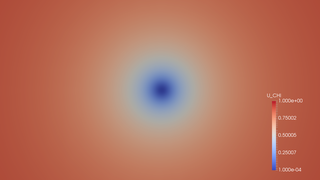
\includegraphics[width=0.8\textwidth]{figs/AE/sbh_boost/img_slice_000050.png}
		}
	\end{minipage}
	\begin{minipage}{0.32\linewidth}
		\subfloat[{$\SS=1000,\ \TT=43.94~M$}] {
			
\includegraphics[width=0.8\textwidth]{figs/AE/sbh_boost/img_slice_000100.png}
		}
	\end{minipage} \hfill

	\begin{minipage}{0.32\linewidth}
			\subfloat[{$\SS=1500,\ \TT=65.91~M$}] {
				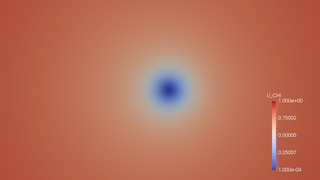
\includegraphics[width=0.8\textwidth]{figs/AE/sbh_boost/img_slice_000150.png}
			}
		\end{minipage}
		\begin{minipage}{0.32\linewidth}
			\subfloat[{$\SS=2000,\ \TT=87.88~M$}] {
				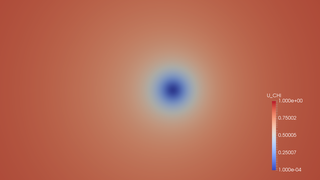
\includegraphics[width=0.8\textwidth]{figs/AE/sbh_boost/img_slice_000200.png}
			}
		\end{minipage}
		\begin{minipage}{0.32\linewidth}
			\subfloat[{$\SS=2500,\ \TT=109.85~M$}] {
				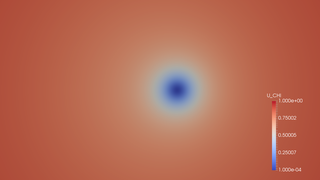
\includegraphics[width=0.8\textwidth]{figs/AE/sbh_boost/img_slice_000250.png}
			}
		\end{minipage} \hfill
	
	\begin{minipage}{0.32\linewidth}
		\subfloat[{$\SS=3000,\ \TT=131.82~M$}] {
			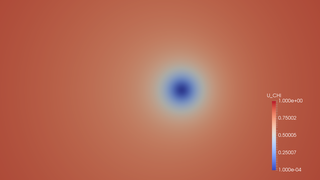
\includegraphics[width=0.8\textwidth]{figs/AE/sbh_boost/img_slice_000300.png}
		}
	\end{minipage}
	\begin{minipage}{0.32\linewidth}
		\subfloat[{$\SS=3500,\ \TT=153.79~M$}] {
			
\includegraphics[width=0.8\textwidth]{figs/AE/sbh_boost/img_slice_000350.png}
		}
	\end{minipage}
	\begin{minipage}{0.32\linewidth}
		\subfloat[{$\SS=4000,\ \TT=175.76~M$}] {
			
\includegraphics[width=0.8\textwidth]{figs/AE/sbh_boost/img_slice_000400.png}
		}
	\end{minipage} \hfill
	
	
	\begin{minipage}{0.32\linewidth}
		\subfloat[{$\SS=4500,\ \TT=197.73~M$}] {
			
\includegraphics[width=0.8\textwidth]{figs/AE/sbh_boost/img_slice_000450.png}
	}
	\end{minipage}
	\begin{minipage}{0.32\linewidth}
		\subfloat[{$\SS=5000,\ \TT=219.70~M$}] {
			
\includegraphics[width=0.8\textwidth]{figs/AE/sbh_boost/img_slice_000500.png}
		}
	\end{minipage}
	\begin{minipage}{0.32\linewidth}
		\subfloat[{$\SS=5500,\ \TT=241.67~M$}] {
			
\includegraphics[width=0.8\textwidth]{figs/AE/sbh_boost/img_slice_000550.png}
	}
	\end{minipage} \hfill
	
		\begin{minipage}{0.32\linewidth}
			\subfloat[{$\SS=6000,\ \TT=263.64~M$}] {
				
\includegraphics[width=0.8\textwidth]{figs/AE/sbh_boost/img_slice_000600.png}
			}
		\end{minipage}
		\begin{minipage}{0.32\linewidth}
			\subfloat[{$\SS=6500,\ \TT=285.61~M$}] {
				
\includegraphics[width=0.8\textwidth]{figs/AE/sbh_boost/img_slice_000649.png}
			}
		\end{minipage} \hfill
%		\begin{minipage}{0.32\linewidth}
%			\subfloat[{$\SS=550$}] {
%				
\includegraphics[width=0.8\textwidth]{figs/AE/sbh_boost/img_slice_000550.png}
%			}
%		\end{minipage} \hfill
	
	\caption{A single black hole boosted in the $x$-direction, with \maxDepth=12 and wavelet tolerance of $10^{-3}$. Time is given in terms of the black hole
mass, $M$. \label{fig:sbh_boost}}
\end{figure*}





\begin{figure*}
	\begin{minipage}{0.32\linewidth}
		\subfloat[{$\SS=0,\ \TT=0~M$}] {
			
\includegraphics[width=0.8\textwidth]{figs/AE/r1/img_slice_000000.png}
		}
	\end{minipage}
	\begin{minipage}{0.32\linewidth}
		\subfloat[{$\SS=500,\ \TT=21.97~M$}] {
			
\includegraphics[width=0.8\textwidth]{figs/AE/r1/img_slice_000010.png}
		}
	\end{minipage}
	\begin{minipage}{0.32\linewidth}
		\subfloat[{$\SS=1000,\ \TT=43.94~M$}] {
			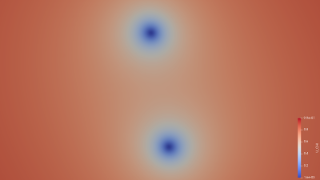
\includegraphics[width=0.8\textwidth]{figs/AE/r1/img_slice_000020.png}
		}
	\end{minipage} \hfill
	
	\begin{minipage}{0.32\linewidth}
		\subfloat[{$\SS=1500,\ \TT=65.91~M$}] {
			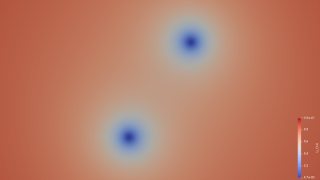
\includegraphics[width=0.8\textwidth]{figs/AE/r1/img_slice_000030.png}
		}
	\end{minipage}
	\begin{minipage}{0.32\linewidth}
		\subfloat[{$\SS=2000,\ \TT=87.88~M$}] {
			
\includegraphics[width=0.8\textwidth]{figs/AE/r1/img_slice_000040.png}
		}
	\end{minipage}
	\begin{minipage}{0.32\linewidth}
		\subfloat[{$\SS=2500,\ \TT=109.85~M$}] {
			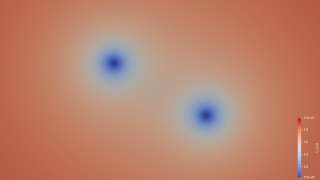
\includegraphics[width=0.8\textwidth]{figs/AE/r1/img_slice_000050.png}
		}
	\end{minipage} \hfill
	
	\begin{minipage}{0.32\linewidth}
		\subfloat[{$\SS=3000,\ \TT=131.82~M$}] {
			
\includegraphics[width=0.8\textwidth]{figs/AE/r1/img_slice_000060.png}
		}
	\end{minipage}
	\begin{minipage}{0.32\linewidth}
		\subfloat[{$\SS=3500,\ \TT=153.79~M$}] {
			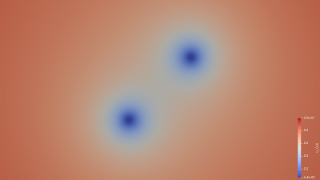
\includegraphics[width=0.8\textwidth]{figs/AE/r1/img_slice_000070.png}
		}
	\end{minipage}
	\begin{minipage}{0.32\linewidth}
		\subfloat[{$\SS=4000,\ \TT=175.76~M$}] {
			
\includegraphics[width=0.8\textwidth]{figs/AE/r1/img_slice_000080.png}
		}
	\end{minipage} \hfill
	
	
	\begin{minipage}{0.32\linewidth}
		\subfloat[{$\SS=4500,\ \TT=197.73~M$}] {
			
\includegraphics[width=0.8\textwidth]{figs/AE/r1/img_slice_000090.png}
		}
	\end{minipage}
	\begin{minipage}{0.32\linewidth}
		\subfloat[{$\SS=5000,\ \TT=219.70~M$}] {
			
\includegraphics[width=0.8\textwidth]{figs/AE/r1/img_slice_000100.png}
		}
	\end{minipage}
	\begin{minipage}{0.32\linewidth}
		\subfloat[{$\SS=5500,\ \TT=241.67~M$}] {
			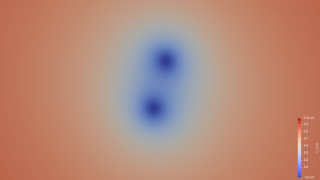
\includegraphics[width=0.8\textwidth]{figs/AE/r1/img_slice_000110.png}
		}
	\end{minipage} \hfill

	\caption{This figure shows frames from the evolution of a black hole
binary with an equal mass ratio, $q=1$. Time is measured in terms of the total
black hole mass $M$.\label{fig:r1}	}
\end{figure*}


\begin{figure*}
	\begin{minipage}{0.32\linewidth}
		\subfloat[{$\SS=0,\ \TT=0~M$}] {
			
\includegraphics[width=0.8\textwidth]{figs/AE/r10/img_slice_000000.png}
		}
	\end{minipage}
	\begin{minipage}{0.32\linewidth}
		\subfloat[{$\SS=500,\ \TT=21.97~M$}] {
			
\includegraphics[width=0.8\textwidth]{figs/AE/r10/img_slice_000010.png}
		}
	\end{minipage}
	\begin{minipage}{0.32\linewidth}
		\subfloat[{$\SS=1000,\ \TT=43.94~M$}] {
			
\includegraphics[width=0.8\textwidth]{figs/AE/r10/img_slice_000020.png}
		}
	\end{minipage} \hfill
	
	\begin{minipage}{0.32\linewidth}
		\subfloat[{$\SS=1500,\ \TT=65.91~M$}] {
			
\includegraphics[width=0.8\textwidth]{figs/AE/r10/img_slice_000030.png}
		}
	\end{minipage}
	\begin{minipage}{0.32\linewidth}
		\subfloat[{$\SS=2000,\ \TT=87.88~M$}] {
			
\includegraphics[width=0.8\textwidth]{figs/AE/r10/img_slice_000040.png}
		}
	\end{minipage}
	\begin{minipage}{0.32\linewidth}
		\subfloat[{$\SS=2500,\ \TT=109.85~M$}] {
			
\includegraphics[width=0.8\textwidth]{figs/AE/r10/img_slice_000050.png}
		}
	\end{minipage} \hfill
	
	\begin{minipage}{0.32\linewidth}
		\subfloat[{$\SS=3000,\ \TT=131.82~M$}] {
			
\includegraphics[width=0.8\textwidth]{figs/AE/r10/img_slice_000060.png}
		}
	\end{minipage}
	\begin{minipage}{0.32\linewidth}
		\subfloat[{$\SS=3500,\ \TT=153.79~M$}] {
			
\includegraphics[width=0.8\textwidth]{figs/AE/r10/img_slice_000070.png}
		}
	\end{minipage}
	\begin{minipage}{0.32\linewidth}
		\subfloat[{$\SS=4000,\ \TT=175.76~M$}] {
			
\includegraphics[width=0.8\textwidth]{figs/AE/r10/img_slice_000080.png}
		}
	\end{minipage} \hfill
	
	
	\begin{minipage}{0.32\linewidth}
		\subfloat[{$\SS=4500,\ \TT=197.73~M$}] {
			
\includegraphics[width=0.8\textwidth]{figs/AE/r10/img_slice_000090.png}
		}
	\end{minipage}
	\begin{minipage}{0.32\linewidth}
		\subfloat[{$\SS=5000,\ \TT=219.70~M$}] {
			
\includegraphics[width=0.8\textwidth]{figs/AE/r10/img_slice_000100.png}
		}
	\end{minipage}
	\begin{minipage}{0.32\linewidth}
		\subfloat[{$\SS=5500,\ \TT=241.67~M$}] {
			
\includegraphics[width=0.8\textwidth]{figs/AE/r10/img_slice_000100.png}
		}
	\end{minipage} \hfill
	

	\caption{This figure shows frames from the evolution of a black hole
binary with mass ratio $q=10$. Time is measured in terms of the total
black hole mass $M$.\label{fig:r10}}
\end{figure*}




\begin{figure*}
	\begin{minipage}{0.32\linewidth}
		\subfloat[{$\SS=0,\ \TT=0~M$}] {
			
\includegraphics[width=0.8\textwidth]{figs/AE/r100/img_slice_000000.png}
		}
	\end{minipage}
	\begin{minipage}{0.32\linewidth}
		\subfloat[{$\SS=500,\ \TT=21.97~M$}] {
			
\includegraphics[width=0.8\textwidth]{figs/AE/r100/img_slice_000020.png}
		}
	\end{minipage}
	\begin{minipage}{0.32\linewidth}
		\subfloat[{$\SS=1000,\ \TT=43.94~M$}] {
			
\includegraphics[width=0.8\textwidth]{figs/AE/r100/img_slice_000040.png}
		}
	\end{minipage} \hfill

	\begin{minipage}{0.32\linewidth}
		\subfloat[{$\SS=1500,\ \TT=65.91~M$}] {
			
\includegraphics[width=0.8\textwidth]{figs/AE/r100/img_slice_000060.png}
		}
	\end{minipage} 
	\begin{minipage}{0.32\linewidth}
		\subfloat[{$\SS=2000,\ \TT=87.88~M$}] {
			
\includegraphics[width=0.8\textwidth]{figs/AE/r100/img_slice_000080.png}
		}
	\end{minipage}
	\begin{minipage}{0.32\linewidth}
		\subfloat[{$\SS=2500,\ \TT=109.85~M$}] {
			\includegraphics[width=0.8\textwidth]{figs/AE/r100/img_slice_000100.png}
		}
	\end{minipage} \hfill

	\begin{minipage}{0.32\linewidth}
		\subfloat[{$\SS=3000,\ \TT=131.82~M$}] {
			\includegraphics[width=0.8\textwidth]{figs/AE/r100/img_slice_000120.png}
		}
	\end{minipage}
	\begin{minipage}{0.32\linewidth}
		\subfloat[{$\SS=3500,\ \TT=153.79~M$}] {
			\includegraphics[width=0.8\textwidth]{figs/AE/r100/img_slice_000140.png}
		} 
	\end{minipage} 
	\begin{minipage}{0.32\linewidth}
		\subfloat[{$\SS=4000,\ \TT=175.76~M$}] {
			\includegraphics[width=0.8\textwidth]{figs/AE/r100/img_slice_000160.png}
		}
	\end{minipage} \hfill

	\begin{minipage}{0.32\linewidth}
		\subfloat[{$\SS=4500,\ \TT=197.73~M$}] {
			\includegraphics[width=0.8\textwidth]{figs/AE/r100/img_slice_000180.png}
		}
	\end{minipage}
	\begin{minipage}{0.32\linewidth}
		\subfloat[{$\SS=5000,\ \TT=219.70~M$}] {
			\includegraphics[width=0.8\textwidth]{figs/AE/r100/img_slice_000200.png}
		}
	\end{minipage}
	\begin{minipage}{0.32\linewidth}
		\subfloat[{$\SS=5500,\ \TT=241.67~M$}] {
			\includegraphics[width=0.8\textwidth]{figs/AE/r100/img_slice_000220.png}
		}
	\end{minipage}\hfill
 
	\caption{This figure shows frames from the evolution of a black hole binary 
with mass ratio $q=100$. Time is given
in terms of the total mass $M$.\label{fig:r100}}
\end{figure*}











\subsection{Boosted Single Black Hole}
\label{sec:AE_sbhboost}

The next experiment is an extension of the single BH test;
it ``boosts'' the BH with constant velocity in $x$-direction.
The constant velocity of the BH should be apparent in the evolution. 
The parameter file for this test can be found in the repository at 
\texttt{SC18\_AE/par/single\_bh1\_boost.par}.
The black hole parameters are given below (note
that $BSSN\_BH1$ has a momentum of 0.114 in $x$-direction).

\begin{lstlisting}[basicstyle=\small]
"BSSN_BH1": { "MASS":1.0, "X":0.0, "Y":0.0, 
"Z": 0.00123e-6, "V_X": 0.114, "V_Y": 0.0, 
"V_Z": 0.0, "SPIN": 0, 
"SPIN_THETA":0, "SPIN_PHI": 0 },

"BSSN_BH2": { "MASS":1e-15,"X":1e15, "Y":0.0, 
"Z":0.00123e-6, "V_X": 0.0, "V_Y": 0.0, 
"V_Z": 0.0, "SPIN": 0, 
"SPIN_THETA":0, "SPIN_PHI": 0 }
\end{lstlisting}



\subsection{Constraint equations}

Similar to the Maxwell equations of electrodynamics, the Einstein equations
contain both hyperbolic evolution equations and elliptic constraint equations,
which must be satisfied at all times. Following the common practice in
numerical relativity, we evolve the hyperbolic equations and monitor the 
quality of the solution by checking that the constraint equations are 
satisfied. The choice of coordinates for the BBH evolution (the puncture gauge) 
does induce constraint violations in the vicinity of each black hole.
The violations of the constraint equations in our runs are consistent with 
the discretization error expected for the numerical derivatives in the
constraint equations and the constraint violations near the black holes 
(punctures). An example of monitored constraint violations are listed in the Table \ref{tb:constraints}.

\begin{table}
	\centering
\scalebox{0.9}{
	\begin{tabular}{||c | c | c | c| c||} 
		\hline
		Time (M) & $\norm{\mathcal{H}_{r>a}}_2$ & $\norm{M1_{r>a}}_2$ & $\norm{M2_{r>a}}_2$ & $\norm{M3_{r>a}}_2$ \\
		\hline\hline
		0 & 0.000777861 & 1.01855e-05 & 1.23443e-05 & 7.17572e-06 \\
		0.976562 & 0.000808294 & 3.05681e-05 & 2.91217e-05 & 2.79631e-05 \\
		1.95312 & 0.000793783 & 5.03912e-05 & 3.93872e-05 & 4.06693e-05 \\
		2.92969 & 0.00079551 & 7.54643e-05 & 5.068e-05 & 5.42466e-05 \\
		3.90625	& 0.000956987 & 0.000102901 & 7.38208e-05 & 7.47156e-05 \\
		4.88281 & 0.00247348 & 0.000200055	& 0.000140583 & 0.000139008 \\
		\hline
	\end{tabular}
}
\caption{Violation of constraint equations with time for an equal mass ratio binary merger simulation done using OT. Note that $\mathcal{H}$, $M1,M2,M3$ denotes the Hamiltonian \& 3 momentum component constraints that is being monitored through the evolution.}
\label{tb:constraints}
\end{table}





\subsection{Binary black holes with mass ratio $q=1$}

We performed a series of short-term binary BH evolutions with different
mass ratios. This run was used to validate the code by comparing the
trajectories of the BHs calculated using \dendro\ to the trajectories calculated
by \HAD. Frames from the evolution are shown in the Figure~\ref{fig:r1},
%the figure,
and the BH parameters used for this run are listed below.

\begin{lstlisting}[basicstyle=\small]
  "BSSN_BH1": {
    "MASS":0.485,
    "X": 4.00e+00, "Y":0.0, "Z": 1.41-05,
    "V_X": -0.00133, "V_Y": 0.112, "V_Z": 0,
    "SPIN": 0, "SPIN_THETA":0, "SPIN_PHI": 0 },
  "BSSN_BH2": {
      "MASS":0.485,
      "X":-4.00+00, "Y":0.0, "Z":1.41-05,
      "V_X": 0.00132, "V_Y": -0.112, "V_Z": 0,
      "SPIN": 0, "SPIN_THETA":0, "SPIN_PHI": 0 }
\end{lstlisting}


\subsection{Binary black holes with mass ratio $q=10$}

We performed a short simulation with a mass ratio $q=10$
This is a short demonstration run to show that \dendro\
easily handles large mass ratios and gives consistent
results for the binary evolution.
Frames from the evolution are shown in figure,
and the BH parameters used for this run are listed below.

\begin{lstlisting}[basicstyle=\small]
  "BSSN_BH1": {
    "MASS":0.903,
    "X":5.45-01, "Y":0.0, "Z": 1.41-05,
    "V_X": -3.90e-04, "V_Y": 0.0470, "V_Z": 0,
    "SPIN": 0, "SPIN_THETA":0, "SPIN_PHI": 0 },
  "BSSN_BH2": {
      "MASS":0.0845,
      "X":-5.45+00, "Y":0.0, "Z":1.41-05,
      "V_X": 3.90e-04, "V_Y": -0.0470, "V_Z": 0,
      "SPIN": 0, "SPIN_THETA":0, "SPIN_PHI": 0 }
\end{lstlisting}

\subsection{Binary black holes with mass ratio $q=100$}

We performed a short simulation with a mass ratio $q=100$
This is a short demonstration run to show that \dendro\ 
produces the proper grid structure for this system and
reasonable results for a very challenging binary configuration.
Frames from the evolution are shown in the figure
and the BH parameters used for this run are listed below.


\begin{lstlisting}[basicstyle=\small]
  "BSSN_BH1": {
    "MASS":0.989,
    "X":5.94-02, "Y":0.0, "Z": 1.41-05,
    "V_X": -5.60-06, "V_Y": 5.61-03, "V_Z": 0,
    "SPIN": 0, "SPIN_THETA":0, "SPIN_PHI": 0 },
  "BSSN_BH2": {
      "MASS":0.00914,
      "X":-5.94+00, "Y":0.0, "Z":1.41421356e-05,
      "V_X": 5.60-06, "V_Y": -5.61-03, "V_Z": 0,
      "SPIN": 0, "SPIN_THETA":0, "SPIN_PHI": 0 }
\end{lstlisting}




% that's all folks
\end{document}


